%%
% The BIThesis Template for Graduate Thesis
%
% Copyright 2020-2023 Yang Yating, BITNP
%
% This work may be distributed and/or modified under the
% conditions of the LaTeX Project Public License, either version 1.3
% of this license or (at your option) any later version.
% The latest version of this license is in
%   https://www.latex-project.org/lppl.txt
% and version 1.3 or later is part of all distributions of LaTeX
% version 2005/12/01 or later.
%
% This work has the LPPL maintenance status `maintained'.
%
% The Current Maintainer of this work is Feng Kaiyu.
%
% Compile with: xelatex -> biber -> xelatex -> xelatex

% !TeX program = xelatex
% !BIB program = biber

% 硕士论文模板 type=master
% 博士论文模板 type=doctor
% 开启盲审格式 blindPeerReview=true (如:[type=master,blindPeerReview=true])
% 开启双面打印模式 twoside=true (如:[type=master,twoside=true])
%     在双面打印模式下,需要放在奇数页的页面后会自动插入一个空白页,以方便直接在打印机上“双面打印”。
%
% 在 Linux 和 macOS 系统下,由于版权问题,中文字体和 Windows 系统下的字体不同。
% 如果想要获得与 Word 文档相同的效果,你有两个选择:
% 1. 使用 Windows 系统编译最终的论文。
% 2. 自己手动安装中易字库并添加选项:`\documentclass[...,ctex={fontset=windows}]{bithesis}`。
%
% **更多使用说明请参考 bithesis.pdf **

\documentclass[type=master,twoside=false]{bithesis}

% 此处仅列出常用的配置。全部配置用法请见「bithesis.pdf」手册。
\BITSetup{
  cover = {
    %% 使用以下参数来自定义封面日期
    date = 2025年6月,
    autoWidthPadding = 0.25em,
  },
  info = {
    % 想要删除某项封面信息,直接删除该项即可。
    % 想要让某项封面信息留空(但是保留下划线),请传入空白符组成的字符串,如"{~}"。
    % 如需要换行,则用 “\\” 符号分割。
    classification = TQ028.1,
    UDC = 540,
    title = 面向学生作文的模型改写检测方法,
    % 如需覆盖竖排标题,请配置以下选项。
    % 下面的例子展示了如何在竖排标题中使用垂直或者旋转的英文。
    % verticalTitle = {形状记忆聚氨酯{L } {T } {X }的合成 \rotatebox[origin=c]{-90}{Feng Kaiyu} 及其在织物中的应用},
    titleEn = {A Method for Detecting Model-Polished Texts in Student Compositions},
    author = 卢品仁,
    authorEn = Pinren Lu,
    studentId = 3120220953,
    school = 计算机学院,
    schoolEn = {School of Computer \\ Science and Technology},
    supervisor = 李侃~教授,  % 指导教师
    supervisorEn = Prof. Kan Li,
    chairman = 高影繁~研究员,  % 答辩委员会主席
    chairmanEn = Research Fellow Yingfan Gao,
    % -------------
    % 请按自身研究生类型填写以下项目
    %
    % --- 学术型 ---
    degreeType = academic,
    degree = 工学硕士,  % 申请学位
    degreeEn = Master of Science in Engineering,
    major = 计算机科学与技术,  % 一级学科
    majorEn = Computer Science and Technology,
    %
    % --- 专业型 ---
    % degreeType = professional,
    % industrialMentor = 李五教授,  % 行业合作导师
    % industrialMentorEn = Prof. Wu Li,
    % degree = 计算机科学与技术硕士,  % 申请类别
    % degreeEn = {Master of Computer \\ Science and Technology},
    % major = 计算机科学与技术,  % 学位领域
    % majorEn = Computer Science and Technology,
    % -------------
    %
    % 如果想要手动控制盲审模式下的隐藏信息,可以使用宏 \SecretInfo{}。使用方式有两种,如:
    % major = \SecretInfo{材料科学与工程} 可以得到 ******* (用等量的替换符号替代)
    % major = \SecretInfo{材料科学与工程}[ABCDEF] 可以得到 ABCDEF (用你自定义的内容替代)
    %
    defenseDate = 2025年6月,
    defenseDateEn = {June, 2025},
    keywords = {大语言模型;文本检测;文本改写},
    keywordsEn = large language model; text detect; text polish,
    %
    % 必要时置于封面右上角,并按照国家规定进行标记。
    % classifiedLevel = 密级\BigStar 保密期限,
    %
    % 特别类型——工程硕博士专项
    % 工程硕博士专项 = true,
    % 特别类型——交叉研究方向(一般不用勾选)
    % crossResearch = true,
    % 特别类型——政府项目留学生(一般不用勾选)
    % internationalStudentUGP = true,
    % 以上三个选项不勾选时将会隐藏显示。
  },
  % 在目录页中不显示摘要和主要符号对照表的标题。
  TOC = {
    abstract = false,
    abstractEn = false,
    symbols = false,
  },
  style = {
    pageVerticalAlign = top,
    % 开启 Windows 平台下的中易宋体伪粗体。
    % windowsSimSunFakeBold = true,
    % 开启该选项后,将用 Times New Roman 的开源字体 TeX Gyre Termes 作为正文字体。
    % 这个选项适用于以下情况:
    % 1. 不想在系统中安装 Times New Roman。
    % 2. 在 Linux/macOS 下遇到 `\textsc` 无法正常显示的问题。
    % betterTimesNewRoman = true,
  },
  publications = {
    % 以下两个选项将影响「攻读学位期间发表论文与研究成果清单」中名称列表的省略阈值。
    % 一般来说,如果你在全部文献中最低排在第四位,建议你将两个值都设置为大于等于 4 的值。
    % 更详细的说明请见手册。
    maxbibnames = 10,
    minbibnames = 10,
    % 「攻读学位期间发表论文与研究成果清单」默认按学校要求,“按发表的时间顺序列出”。
    % 如需调整,可修改以下选项,详见 https://bithesis.bitnp.net/faq/bib-sort.html
    % sorting = false
  },
  % 采用章节标题级别的附录格式
  appendices / chapterLevel = true,
  const = {
    % 关于题名页的字段名称,截至2025年三月末,以下几项规定不完全一致:
    %     Word 模板(学位论文模版-{学术型,专业型}-2025.doc)、研函〔2018〕60号《北京理工大学研究生学位论文撰写规范》、GB/T 7713.1—2006《学位论文编写规则》
    % 目前的默认值按照 Word 模板,可能需要手动调整。
    % 例如取消注释下一行,会将「申请学位/类别」改为「申请学位级别」。
    % info / degree = {申\hspace{0.45ex}请\hspace{0.45ex}学\hspace{0.45ex}位\hspace{0.45ex}级\hspace{0.45ex}别},
    % 详见 https://bithesis.bitnp.net/faq/edit-const.html
  },
  misc = {
    % 关闭后,链接会用多种颜色表示,便于检查。
    % 无论是否开启,都不会影响打印效果。
    hideLinks = true,
    % 微调表格行间距
    tabularRowSeparation = 1.6,
  }
}

% 大部分关于参考文献样式的修改,都可以通过此处的选项进行配置。
% 详情请搜索「biblatex-gb7714-2015 文档」进行阅读。
\usepackage[
  defernumbers=true,
  backend=biber,
  style=gb7714-2015,
  gbalign=gb7714-2015,
  gbnamefmt=lowercase,
  gbpub=false,
  gbannote=true,
  gbpunctin=false,
  doi=false,
  url=false,
  eprint=false,
  isbn=false,
]{biblatex}

% 添加参考文献
\addbibresource{reference/main.bib}
% 攻读学位期间发表论文与研究成果清单,详细使用方法见 `chapters/pub.tex`。
\addbibresource{reference/pub.bib}


\usepackage{algorithm}
\usepackage{algorithmicx}
\usepackage{algpseudocode}

\usepackage{graphicx}
\usepackage{subfig}
\usepackage{float}
\usepackage[normalem]{ulem}

\begin{document}

% 封面绘制
\MakeCover

% 打印书脊
\MakePaperBack

% 中文信息与英文信息
\MakeTitle

% 论文原创性声明和使用授权
\MakeOriginality

%%%%%%%%%%%%%%%%%%%%%%%%%%%%%%
%% 前置部分
%%%%%%%%%%%%%%%%%%%%%%%%%%%%%%
\frontmatter

% 摘要
%%
% The BIThesis Template for Graduate Thesis
%
% Copyright 2020-2023 Yang Yating, BITNP
%
% This work may be distributed and/or modified under the
% conditions of the LaTeX Project Public License, either version 1.3
% of this license or (at your option) any later version.
% The latest version of this license is in
%   https://www.latex-project.org/lppl.txt
% and version 1.3 or later is part of all distributions of LaTeX
% version 2005/12/01 or later.
%
% This work has the LPPL maintenance status `maintained'.
%
% The Current Maintainer of this work is Feng Kaiyu.

\begin{abstract}
  生成式语言模型迅速的发展,促使生成的内容几乎无法与人类撰写的文本区分。这引发了教育工作者对学生提交作品真实性的重大担忧。因此,解决教育领域中对人工智能生成文本(AIGT)的滥用问题已成为当务之急。目前的检测策略主要集中在整篇文档上,这并未完全满足实际需求。由于学生在将AI生成的内容纳入自己的论文之前,可能会对其进行一定程度的修改,因此细粒度检测,特别是在句子级别的检测,显得尤为重要。因此,检测生成文本语言模型的任务越来越受到关注。针对以上问题,本研究提出了教育领域内生成文本语言模型检测的任务,取得了如下研究成果:
  
  (1)针对目前模型改写文本检测数据集仅能分辨是否由大语言模型生成而无法判断由哪个特定大语言模型生成,以及细粒度文本数据集不足这两个问题,构建了相应的数据集,命名为模型改写文本检测数据集,英文名称为 TOSWT(Tracing the Origins of Students’ Writing Texts)。该数据集包含由五个杰出的语言模型生成的文本,基于学生撰写的论证性论文,共包含53,328个文档级和147,976个句子级的数据样本。

  (2)研究通过在文档级和句子级数据上进行实验评估,评估了多种深度学习检测模型,并提出一种双模型特征融合方法。最终结果表明,文本来源追踪的任务极具挑战性,其中句子级任务尤其困难。
  
  (3)为便于用户操作,本文还实现了一个文本改写检测系统。需求分析、系统架构设计以及各模块和接口的设计均在文中进行了详细阐述。该系统的实现基于Flask框架,前端采用Vue.js进行开发,后端则使用Python编程语言。系统的主要功能包括文本改写和文本改写检测。该系统的设计与实现为后续研究奠定了坚实的基础。
\end{abstract}

% 如需手动控制换行连字符位置,可写 aa\-bb,详见
% https://bithesis.bitnp.net/faq/hyphen.html

\begin{abstractEn}
  The rapid advancement of generative language models has made AI-generated content nearly indistinguishable from human-written text. This has raised significant concerns among educators regarding the authenticity of students' submitted work. Consequently, addressing the misuse of AI-generated text (AIGT) in education has become an urgent priority. Current detection strategies primarily focus on entire documents, which do not fully meet practical needs. Since students may modify AI-generated content before incorporating it into their essays, fine-grained detection---particularly at the sentence level---is crucial. As a result, the task of detecting generative text has garnered increasing attention.
  
  To address these challenges, this study proposes a task for detecting AI-generated text in the educational domain and achieves the following key contributions:
  
  (1) Dataset Construction: Existing datasets for rewritten text detection can only determine whether a text is generated by a large language model (LLM) but fail to identify the specific source model. Additionally, there is a lack of fine-grained text datasets. To mitigate these issues, we construct a new dataset named TOSWT (Tracing the Origins of Students' Writing Texts), which includes texts generated by five prominent language models based on students' argumentative essays. The dataset comprises 53,328 document-level and 147,976 sentence-level samples.
  
  (2) Model Evaluation and Fusion Method: Through experiments on document-level and sentence-level data, we evaluate multiple deep learning detection models and propose a dual-model feature fusion approach. The results demonstrate that tracing the origin of text is highly challenging, with the sentence-level task being particularly difficult.
  
  (3) System Implementation: To facilitate user interaction, we develop a text rewriting detection system. The paper elaborates on requirement analysis, system architecture design, and the implementation of modules and interfaces. The system is built using the Flask framework for the backend (Python) and Vue.js for the frontend. Its core functionalities include text rewriting and text rewriting detection, providing a robust foundation for future research.
\end{abstractEn}


% 制作目录
\MakeTOC

% 插图目录
\listoffigures
% 表格目录
\listoftables

% 主要符号对照表
%%
% The BIThesis Template for Graduate Thesis
%
% Copyright 2020-2023 Yang Yating, BITNP
%
% This work may be distributed and/or modified under the
% conditions of the LaTeX Project Public License, either version 1.3
% of this license or (at your option) any later version.
% The latest version of this license is in
%   https://www.latex-project.org/lppl.txt
% and version 1.3 or later is part of all distributions of LaTeX
% version 2005/12/01 or later.
%
% This work has the LPPL maintenance status `maintained'.
%
% The Current Maintainer of this work is Feng Kaiyu.

\begin{symbols}
  \item[AI] 人工智能
  \item[LLM] 大语言模型
  \item[NLP] 自然语言处理
  \item[OpenAI] 开发 ChatGPT 的国外公司
  \item[ChatGPT] 由 OpenAI 开发有历史意义的大语言模型
  \item[AIGT] 人工智能生成文本
  \item[Token] 词元
  \item[TOSWT] 追踪学生写作文本来源数据集
\end{symbols}



\mainmatter

% 请根据论文内容,按照顺序添加章节。
%%==================================================
%% chapter01.tex for BIT Master Thesis
%% modified by yang yating
%% version: 0.1
%% last update: Dec 25th, 2016
%%==================================================
% 1. 绪论
%    1. 研究背景及意义
%       1. 研究背景
%       2. 研究意义
%    2. 国内外研究现状
%    3. 研究内容及主要贡献
%       1. 数据集
%       2. 分类实验
%       3. 评分实验
%    4. 论文组织结构

\chapter{绪论}
\label{chap:intro}

\section{研究背景及意义}

近年来,基于大型语言模型(Large Language Models,LLMs)的生成式自然语言处理(Generative Natural Language Processing,NLP)系统在技术上取得了显著的进展。这些进步从初期的普通语言模型,如 Transformer \cite{transformer}、GPT \cite{gpt}、GPT-2 \cite{gpt2}、GPT-3 \cite{gpt3},逐步演化到更为复杂和强大的模型,如 ChatGPT \cite{chatgpt}、GPT-4 \cite{openai2024gpt4} 和 DeepSeek V3 \cite{deepseekai2024deepseekv3technicalreport}。这些先进的语言模型生成的文本内容与人类撰写的文本几乎无法区分,表明了人工智能在自然语言处理领域的巨大潜力。这一技术进步已经在多个领域得到了广泛应用,包括聊天机器人、自动内容生成以及文摘工具等,人工智能生成文本(AI-generated texts, AIGT)几乎渗透到我们生活的每一个角落。

然而,对于教育工作者而言,这些技术进展引发了对学生撰写文档真实性的深切担忧。在教育环境中,确保学生的作业和报告反映其真实能力和思维过程变得愈加重要。因此,如何有效避免人工智能生成文本在教育领域的滥用,成为亟待解决的关键问题 \cite{guo_how_2023}。当前的人工智能生成文本检测策略,如基于监督学习的判别器和困惑度测量方法,主要集中于判断整篇文档是否由人工智能生成。然而,现实情况是,用户往往在使用大型语言模型时对部分文本进行修改,而非完全依赖于其生成整个文档 \cite{wang_llm-detector_2024}。这种现象表明,现有检测方法在应对实际应用中的复杂性时可能显得力不从心。

因此,探索细粒度(例如句子级别)的人工智能生成文本检测显得尤为重要 \cite{wang_seqxgpt_2023}。细粒度检测不仅能够为总体检测器提供基础架构,还能够更准确地揭示文本的生成特征和模式。此外,人工智能生成文本的检测效果也可以用作评估其质量的指标:生成的文本越难以被检测出来,表明其与人类文本的一致性越高。

除了检测人工智能生成文本的能力,人工智能文本溯源的任务也逐渐浮出水面。首先,如果仅能检测出文本是由人工智能生成但无法追溯其具体来源,则该检测的说服力将大幅下降。其次,类似于人类学中的溯源概念,识别AI生成文本的来源对于理解文本的生成过程、评估其可信度,以及追踪潜在的偏见和错误至关重要。在教育学领域,为教师提供分析文本来源的工具,不仅能够帮助他们更有效地评估学生的作业和报告,还能识别文本的具体来源,从而判断学生是否过度依赖AI工具进行写作 \cite{li_origin_2023}。这一过程不仅有助于维护学术标准,还能促进学生对原创性和独立思考的重视。

通过深入了解文本的生成背景,教师能够在课堂上进行更有针对性的指导,鼓励学生发展批判性思维能力和创造性写作技巧。因此,本研究旨在探讨基于学生作文数据的人工智能生成文本分类器,旨在为教育工作者提供有效的工具,帮助他们更好地理解和评估学生的写作能力及其背后的生成机制。

\section{国内外研究现状及发展趋势}
\label{sec:intro-inout}

关于使用检测器探测文本是否由人工智能生成的任务,可以从两个主要方面进行深入探讨:文本生成与文本分类。

首先,文本生成涉及到人工智能系统如何利用特定算法和模型生成自然语言文本。这一过程通常依赖于大型语言模型(Large Language Models, LLMs)架构。通过对海量文本数据的学习,这些模型能够捕捉语言的结构和语义特征,从而生成与人类书写风格相似的文本。这一领域的研究不仅关注生成文本的质量和流畅性,还包括生成文本的多样性和上下文适应能力。因此,深入理解文本生成的机制对于评估其潜在的应用和影响至关重要。

另一方面,文本分类是指通过特定的算法和方法对文本进行分析,以确定其是否由人工智能生成。探测文本是否为人工智能生成的任务可以视为一个二分类问题,采用文本分类模型将文本标记为“人类”或“AI”。这一过程通常包括特征提取、模型训练和分类决策等多个步骤。文本分类器可以利用多种技术,包括监督学习和无监督学习方法,这些方法通过分析文本的语言特征、结构特征及其上下文信息来识别文本的生成来源。通过对文本进行分类,研究者能够揭示人工智能生成文本的特征,从而提高检测的准确性和可靠性。

\subsection{文本生成}
\label{sec:intro-inout-textgenerate}

国外在文本生成方面的技术暂时领先于国内。截至目前,大多数富有创新性的工作均由国外提出。追溯到 2017 年,Vaswani等 \cite{transformer} 提出了 Transformer 模型,其核心创新在于自注意力机制,使得模型能够有效处理长距离依赖关系。Transformer 的并行处理能力和高效的特征提取使其成为自然语言处理任务的主流选择。在自然语言处理领域,Transformer 模型的引入标志着一种新的架构设计理念的诞生,其自注意力机制使得模型能够有效捕捉序列中各个元素之间的关系。然而,传统的 Transformer 模型通常依赖于大量标注数据进行任务特定的训练,导致其在不同任务上的适应性和泛化能力受到限制。

为了解决这一问题,国外的研究人员率先开发出预训练模型。通过在大规模未标注文本上进行预训练,预训练模型不仅学习了语言的基本结构和语义,还能够通过微调快速适应多种下游任务。这种两阶段的训练策略和双向上下文理解能力,使得预训练模型在性能和效率上相较于传统模型具有显著优势,推动了自然语言处理技术的进一步发展。预训练模型在自然语言处理领域引起了广泛关注,尤其是BERT\cite{devlin_bert_2019}、BART\cite{lewis-etal-2020-bart}、GPT-1\cite{gpt}、GPT-2\cite{gpt2}和GPT-3\cite{gpt3}等模型的出现,进一步推动了技术的进步。BERT(Bidirectional Encoder Representations from Transformers)基于其独创的双向编码器架构,能够同时考虑上下文的前后信息,极大地提升了文本理解能力。BART(Bidirectional and Auto-Regressive Transformers)则结合了BERT的编码特性和GPT的自回归生成能力,适用于文本生成和序列到序列的任务。GPT-1(Generative Pre-trained Transformer 1)是首个采用自回归生成的预训练模型,奠定了生成模型的基础。随后,GPT-2在规模和性能上进行了显著提升,展示了强大的文本生成能力和广泛的应用潜力。最新的GPT-3则通过1750亿个参数,进一步提升了生成质量和上下文理解,展现出更强的通用性和灵活性,成为当前最先进的自然语言处理模型之一。这些模型的共同特征是通过预训练和微调机制,极大地提高了在各种自然语言处理任务中的表现。

与此同时,在文本生成领域,国内对语言模型和预训练模型的研究也取得了显著的进展,展现出丰富的创新成果。例如,王晓峰 \cite{transformer-cn} 基于 Transformer 模型,深入探讨了其在中文文本生成中的应用。他的研究不仅丰富了中文自然语言处理的理论基础,还为实际应用提供了高效的技术支持,推动了该领域的快速发展。这一工作为后续研究者在中文文本生成任务中提供了重要的参考框架,使得相关技术得以在更广泛的场景中应用。

此外,国内还有研究专注于文本生成的基础架构,进一步推动了该领域的创新。李思慧等 \cite{lisihui-textgenerate} 开发了一种新型的基于凸损失函数的离散扩散文本生成模型。该模型充分利用了凸函数锐化最优分布的特性,使得生成过程更加专注于高概率输出,从而显著提高了文本生成的质量。为了进一步提升生成文本的整体效果并降低生成词的重复率,研究团队设计了一种混合感知噪音表。该表通过引入非线性变化的噪音标记,增强了模型在生成过程中的灵活性和适应性。在解码过程中,他们还采用了一种高置信度的确定性去噪策略,有效地减少了生成文本中的噪音干扰。这一策略不仅提升了文本的流畅性和可读性,还增强了生成内容的多样性和创新性。这些研究成果不仅为中文文本生成提供了新的思路和方法,还为未来的研究和应用奠定了坚实的基础,推动了自然语言处理技术在中文语境下的进一步发展。整体而言,国内在文本生成方面的研究正在不断深化,为推动人工智能的进步贡献着重要力量。

国内的研究更多集中于文本生成模型在实际应用领域的探索。胡妍璐 \cite{huyanlu-textgenerate-news} 在分析文本生成技术在新闻生产中的应用基础上,探讨了大数据环境下的新闻文本生成,旨在构建一种新型且更具影响力的新闻生产模式。张蔚琪 \cite{zhangweiqi} 提出了基于孪生架构与多视图匹配的法律问答模型,利用BERT孪生网络架构和注意力池化层生成多个视图的向量表示,通过细粒度的语义交互提升匹配准确性。此外,她将法律问答建模为生成任务,提出了一种基于迁移学习和改进解码算法的生成式法律问答模型,能够在生成过程中识别并替换过于通用的回复,从而提高回答的相关性。进一步地,张蔚琪构建了带有法条知识标注的法律问答数据集,并提出了一种检索知识驱动的生成式模型。该模型结合了知识检索与答案生成,确保生成的回答既具相关性,又能根据最新法律知识进行调整。这些研究成果为法律智能化建设提供了新的思路,推动了法律问答系统的发展。

预训练模型的成功为大语言模型的出现奠定了基础,后者在此基础上进行了多项重要改进。大语言模型通过更大规模的训练数据和参数量,显著提升了模型的表现能力和生成质量。此外,它们采用了更深层次的网络结构和更复杂的训练策略,例如混合精度训练和分布式训练,以提高训练效率和模型的表达能力。同时,大语言模型在上下文理解方面也进行了优化,能够处理更长的文本输入,增强了对上下文的记忆和推理能力。此外,许多大语言模型引入了更先进的自注意力机制和动态计算图,使得模型在生成文本时更加灵活和高效。这些改进使得大语言模型不仅在自然语言生成任务中表现出色,也在理解、翻译和问答等多种应用场景中展现出强大的能力,推动了人工智能技术的进一步发展。在近年来的自然语言处理领域,多个大型语言模型相继被提出,显著推动了文本生成和理解的研究进展。ChatGPT \cite{chatgpt} 是 OpenAI 开发的对话生成模型,基于生成预训练变换器(GPT)架构,经过大规模对话数据的微调,旨在实现自然流畅的人机交互。其设计重点在于上下文理解和生成能力,使其能够在多种主题下进行有效交流。GPT-4 \cite{openai2024gpt4} 是 OpenAI 推出的第四代生成预训练变换器模型,相较于其前身 GPT-3,GPT-4 在模型规模、性能和上下文处理能力上均有显著提升。该模型能够处理更长的文本输入,并在多种复杂任务中表现出更高的灵活性和准确性,尤其在多模态输入(文本和图像)方面展现出新的潜力。Gemini \cite{geminiteam} 是由 Google DeepMind 开发的一种新型大型语言模型,旨在与现有的 AI 模型竞争。Gemini 结合了先进的技术和架构,强调在自然语言理解和生成任务中的表现,展现出在多领域应用中的强大能力。LLaMA \cite{touvron2023llamaopenefficientfoundation, touvron2023llama2openfoundation, grattafiori2024llama3herdmodels} (Large Language Model Meta AI)是 Meta(前 Facebook)推出的一系列开源大型语言模型,旨在提供高效的语言生成和理解能力。LLaMA 关注于可扩展性和性能,支持多种语言和任务,尤其在资源有限的环境中表现出色。这些模型的不断发展为自然语言处理领域的研究和应用提供了新的视角和方法。

% 文心一言, ChatGLM,通义千问,pangu alpha sigma pi, 

近年来,国内在大语言模型的研究领域取得了显著突破。早在OpenAI推出ChatGPT之前,中国的研究人员便已开始对大语言模型进行探索。由于大型企业拥有丰富的显卡资源,因此其研究进展往往领先于学术界。百度的研究团队率先进入这一领域,提出了文心一言模型\cite{sun2019ernieenhancedrepresentationknowledge, sun2019ernie20continualpretraining, sun2021ernie30largescaleknowledge},该模型具备多模态处理能力,能够有效处理文本、图像等多种数据类型,适应广泛的应用场景。文心一言专门针对中文进行了优化,显著提升了对中文语境的理解和生成效果,展现出卓越的文本生成能力,适合于内容创作和客户服务等多个领域。此外,该模型整合了丰富的知识库,能够在文本生成过程中引用相关知识,从而增强文本的准确性与信息量。其高度的可定制性使得用户能够根据特定需求进行调整,支持实时交互并迅速响应用户输入,从而提升用户体验。这些特性使得文心一言在中文自然语言处理领域具有重要的应用潜力。

在ChatGPT震撼发布后,国内研究人员积极追赶,力求超越OpenAI的研究成果。华为的研究团队提出了盘古模型\cite{zeng2021pangualphalargescaleautoregressivepretrained, wang2023pangupienhancinglanguagemodel, ren2023pangusigmatrillionparameterlanguage},该模型采用了大规模的预训练和微调策略,在多种语言理解和生成任务中表现出色。此外,盘古模型在中文处理方面进行了针对性优化,能够更准确地理解和生成符合中文语境的内容,具备强大的上下文理解能力,能够在复杂对话和长文本生成中保持连贯性。华为团队还深入研究了模型的可扩展性和效率,使其能够在多种硬件平台上高效运行。总体而言,盘古模型为中文自然语言处理提供了强有力的技术支持,推动了相关应用的发展。

在ChatGPT(GPT-3.5)发布的同时,清华大学的研究团队推出了GLM-130B\cite{zeng2023glm130bopenbilingualpretrained},在众多流行的英语基准测试中显著超越了ChatGPT的前一版本GPT-3 175B(davinci)。同时,在相关基准测试中,GLM-130B也始终显著优于当时百度提出的文心一言系列模型中的最大中文语言模型ERNIE TITAN 3.0 260B。基于GLM-130B独特的缩放特性,该模型实现了INT4量化,无需后续训练,几乎没有性能损失,成为首个在100B规模模型中实现这一技术的模型。更为重要的是,这一特性使其能够在4×RTX 3090(24G)或8×RTX 2080 Ti(11G)GPU上进行高效推理,成为当时使用100B规模模型所需的经济高效的GPU选择。

在 OpenAI 发布 GPT-4 之后,国内的大语言模型研究如雨后春笋般蓬勃发展。阿里巴巴的研究团队推出了通义千问系列模型\cite{bai2023qwentechnicalreport}。Qwen 是一个全面的开源语言模型系列,涵盖了不同参数规模的多种模型。其中包括基础的预训练语言模型 Qwen 以及经过人类对齐技术微调的聊天模型 Qwen-Chat。基础语言模型在多项下游任务中始终展现出卓越的性能,而聊天模型,尤其是那些通过强化学习(RLHF)技术结合人类反馈进行训练的模型,竞争极为激烈。这些聊天模型具备创建代理应用程序的高级工具使用与规划能力,甚至在处理复杂任务时,如使用代码解释器的大型模型中,也表现出令人瞩目的性能。此外,团队还开发了专用于编码的模型 Code-Qwen 和 Code-Qwen-Chat,以及基于基础语言模型的数学模型 Math-Qwen-Chat。与当时的其他开源模型相比,通义千问系列模型的性能显著提升,略微落后于专有模型。

紧接着,清华大学的研究团队在 GLM-130B 模型的研究中取得了创新进展,开发了 ChatGLM-RLHF 流程 \cite{hou2024chatglmrlhfpracticesaligninglarge},这是一个基于人类反馈的强化学习(RLHF \cite{kaufmann2024surveyreinforcementlearninghuman})系统,旨在增强 ChatGLM 与人类偏好的对齐一致性。ChatGLM-RLHF 主要包括三个核心组成部分:人类偏好数据的收集、奖励模型的训练以及策略的优化。为降低大规模训练中的奖励方差,采用了通过融合梯度下降实现模型并行性的策略,并设计了正则化约束以防止 LLM 中的灾难性遗忘。实验结果显示,与监督微调(SFT)版本的 ChatGLM 相比,ChatGLM-RLHF 在对齐任务中取得了显著的改进。例如,在中文对齐任务中,其平均表现比 ChatGLM-SFT 提高了 15\%。这项研究展示了国内在根据人类偏好对齐大语言模型方面的实践,为强化学习实施中的挑战与解决方案提供了宝贵的见解。

随后,研究团队在此基础上提出了 GLM-4 大语言模型家族\cite{glm2024chatglmfamilylargelanguage},其中包括 GLM-4、GLM-4-Air 和 GLM-4-9B。这些模型代表了国内最具实力的开源模型,基于前三代 ChatGLM 的所有经验和洞察进行训练。GLM-4 模型在十万亿个主要为中文和英文的令牌上进行了预训练,同时还使用了来自 24 种语言的一小部分语料库,主要针对中文和英文的使用进行了对齐。高质量的对齐是通过多阶段的训练后过程实现的,包括监督微调和从人类反馈中学习。评估结果表明,GLM-4 在 MMLU \cite{hendrycks2021measuringmassivemultitasklanguage}、GSM8K \cite{cobbe2021trainingverifierssolvemath}、MATH \cite{hendrycks2021measuringmathematicalproblemsolving}、BBH \cite{suzgun2022challengingbigbenchtaskschainofthought}、GPQA \cite{rein2023gpqagraduatelevelgoogleproofqa} 和 HumEval \cite{peng2024humanevalxlmultilingualcodegeneration} 等多个通用指标上与 GPT-4 进行了密切竞争,甚至在某些方面优于 GPT-4。在 IFEval \cite{zhou2023instructionfollowingevaluationlargelanguage} 的指令遵循测评中,GLM-4 的表现接近于 GPT-4-Turbo,并在长上下文任务中与 GPT-4 Turbo(128K)和 Claude 3 的表现相当。此外,在对齐 Bench 测量的中文对齐方面,GLM-4 亦优于 GPT-4。在实际应用中,GLM-4 在通过 Web 浏览获取在线信息和使用 Python 解释器解决数学问题等任务中,表现与 GPT-4 All Tools 相当甚至更佳,仅在 2023 年便吸引了超过 1000 万次的 HuggingFace 下载。

% qwen2.5, qwen2.5VL qwq32b, deepseek

在 GPT-o1 \cite{wu2024comparativestudyreasoningpatterns} 发布之后,国内再度掀起了追赶的热潮。OpenAI的o1模型展示了推理策略(即测试时的计算方法)对大型语言模型推理能力的显著提升,其在多数数据集上均取得了最佳性能。对此,国内的大语言模型研究者们积极响应,迅速跟进。首先,阿里巴巴公司的研究团队在其早期开发的通义千问系列模型基础上,推出了通义千问2.5(Qwen 2.5)模型  \cite{qwen2025qwen25technicalreport}。这一系列全面的大语言模型(LLM)旨在满足多样化的需求。与之前的版本相比,Qwen 2.5在训练前和训练后阶段均取得了显著进展。在预训练阶段,模型所使用的高质量数据集从7万亿词元扩展至18万亿词元,为常识、专家知识及推理能力的提升奠定了坚实基础。在后训练阶段,研究团队通过100万个样本实施了复杂的监督微调和多阶段强化学习,从而增强了人类偏好,显著改善了长文本生成、结构数据分析及指令遵循能力。为了有效应对多样化的应用场景,研究者们推出了不同规模的Qwen 2.5 LLM系列,开放权重的产品包括基础模型和指令调整模型,并提供量化版本。此外,托管方案中还包括两种混合专家(MoE)变体:Qwen 2.5-Turbo和Qwen 2.5-Plus,均可通过阿里云模型工作室获得。Qwen 2.5在语言理解、推理、数学、编码以及人类偏好对齐等多个基准测试中展现了卓越性能。尤其是开放权重的旗舰Qwen 2.5-72B-Instruct在众多开放和专有模型中表现优异,并与最先进的开放权重模型Llama-3-405B-Instruct \cite{grattafiori2024llama3herdmodels} 竞争,后者的参数量约为其五倍。Qwen 2.5-Turbo和Qwen 2.5-Plus在成本效益方面表现出色,分别与GPT-4o-mini和GPT-4o相抗衡。此外,Qwen 2.5模型为训练专业模型(如Qwen 2.5-Math、Qwen 2.5-Coder、QwQ及多模态模型)提供了重要基础。

在推出这一文本模态的大语言模型之后,阿里巴巴的研究团队为实现与OpenAI的GPT系列模型相媲美的多模态能力,继续深入探索多模态大语言模型的潜力,提出了通义千问2.5 VL \cite{bai2025qwen25vltechnicalreport}。该模型作为Qwen视觉语言系列的最新旗舰,展现了基础功能与创新特性的显著进步。Qwen2.5-VL通过增强的视觉识别、精准的对象定位、强大的文档解析能力及对长视频的理解,实现在理解与世界互动方面的重大突破。Qwen2.5-VL的一个显著特点是其能够通过边界框或点的方式精确定位对象,并具备从图像和表格中提取强大结构化数据的能力。为有效处理复杂输入,该模型引入了动态分辨率处理和绝对时间编码,使其能够通过二级事件定位来处理不同尺寸的图像及持续时间可达数小时的视频。这一设计使得模型能够在无需依赖传统归一化技术的情况下,局部感知空间尺度和时间动态。通过从头训练原生动态分辨率视觉转换器(Vision Transformer, ViT \cite{dosovitskiy2021imageworth16x16words})并结合窗口注意力机制,Qwen2.5-VL在保持原生分辨率的同时有效降低了计算开销。因此,Qwen2.5-VL不仅在静态图像和文档理解方面表现卓越,作为交互式视觉代理,它能够在实际场景中进行推理、工具使用和任务执行,诸如操作计算机和移动设备等。该模型提供三种不同尺寸,以应对从边缘AI到高性能计算的多样化应用场景。旗舰型号Qwen2.5-VL-72B在文档和图表理解方面与GPT-4o及Claude 3.5 Sonnet \cite{AnthropicModelCA}等最先进模型相当,尤其在这些领域表现出色。此外,Qwen2.5-VL在保持强大语言性能的同时,保留了Qwen2.5 LLM的核心语言能力。

在刚刚过去的一年中,杭州深度求索人工智能基础技术研究有限公司经历了技术的“爆炸性”发展,迅速获得了与OpenAI开发的人工智能相媲美的能力。2024年初,该公司推出了DeepSeek模型 \cite{deepseekai2024deepseekllmscalingopensource},其研究深入探讨了缩放定律,并提出了独特的发现,这些发现为在两种广泛使用的开源配置(7B和67B)中扩展大规模模型提供了重要支持。在缩放定律的指导下,研究团队引入了DeepSeek LLM,这是一个旨在从长远角度推进开源语言模型的项目。为了更有效地支持预训练阶段,研究人员开发了一个目前包含2万亿词元的数据集,并持续进行扩展。随后,在 DeepSeek LLM Base 模型的基础上,团队实施了监督微调(SFT)和直接偏好优化(DPO),最终创建了DeepSeek Chat模型。评估结果显示,DeepSeek LLM67B在一系列基准测试中超越了LLaMA-270B,尤其在代码、数学及推理领域表现优异。此外,开放式评估结果表明,与GPT-3.5相比,DeepSeek LLM67B在聊天任务中展现了卓越的性能。

在2024年中,杭州深度求索人工智能基础技术研究有限公司再次取得了技术突破,推出了DeepSeek-V2 \cite{deepseekai2024deepseekv2strongeconomicalefficient},这是一种强大的混合专家(MoE)语言模型,具有经济高效的训练和推理能力。该模型总参数量达到236B,其中每个词元的激活参数为21B,并支持128K词元的上下文长度。DeepSeek-V2采用了多项创新架构,包括多头潜在注意力(MLA)和DeepSeekMoE。MLA通过显著压缩键值(KV)缓存为潜在向量,从而确保高效的推理过程;而DeepSeekMoE则通过稀疏计算以较低的成本训练出强大的模型。与DeepSeek67B相比,DeepSeek-V2在性能上显著提升,同时节省了42.5\%的训练成本,减少了93.3\%的KV缓存,并将最大生成吞吐量提升至5.76倍。该模型在一个由8.1T词元构成的高质量多源语料库上进行了预训练,并进一步实施了监督微调(SFT)和强化学习(RL)以最大限度地发挥其潜力。评估结果显示,即便只有21B的激活参数,DeepSeek-V2及其聊天版本仍在开源模型中展现出顶尖的性能。

在2024年12月,深度求索人工智能基础技术研究有限公司推出了一项重大创新,基于先前开发的DeepSeek模型 \cite{deepseekai2024deepseekllmscalingopensource, deepseekai2024deepseekv2strongeconomicalefficient},开源了与GPT-4o性能相媲美的DeepSeek-V3模型 \cite{deepseekai2024deepseekv3technicalreport}。该模型是一种强大的混合专家(MoE)语言模型,具有总参数量达到671B,其中每个词元激活了37B参数。为实现高效的推理和训练,DeepSeek-V3采用了多头潜在注意力(MLA)和DeepSeekMoE架构,这些架构在DeepSeek-V2中经过了全面验证。此外,DeepSeek-V3引入了一种负载平衡的无辅助损失策略,并设定了多令牌预测的训练目标,以进一步提升模型性能。研究团队在一个包含14.80万亿多样化且高质量词元的语料库上进行了DeepSeek-V3的预训练,随后进行了监督微调和强化学习阶段,以充分发挥其潜力。综合评估结果表明,DeepSeek-V3的性能超越了其他开源模型,并与领先的闭源模型相当。尽管性能卓越,DeepSeek-V3的完整训练仅需2.788M H800 GPU小时。此外,其训练过程表现出极高的稳定性,研究人员在整个训练期间未遇到任何不可恢复的损失峰值或需进行回滚的情况。

紧接着,在刚刚过去的2025年初,深度求索的研究团队向全球发布了其显著成就,开源了与当今全球最强的OpenAI公司所推出的最佳模型GPT-o1相媲美的DeepSeek-R1模型 \cite{deepseekai2025deepseekr1incentivizingreasoningcapability}。此次发布包括了第一代推理模型DeepSeek-R1-Zero和DeepSeek-R1。DeepSeek-R1-Zero是通过大规模强化学习(Reinforcement Learning, RL)训练而成的,且未经过任何初步的有监督微调(Supervised Fine-tuning, SFT),展现出卓越的推理能力。通过强化学习的方式,DeepSeek-R1-Zero自然地表现出许多强大而引人注目的推理行为。然而,该模型也面临可读性差和语言混合等诸多挑战。为了解决这些问题并进一步提升推理性能,研究团队推出了DeepSeek-R1,该模型在强化学习之前结合了多阶段训练和冷启动数据。DeepSeek-R1在推理任务中实现了与OpenAI-o1-1217相当的性能。为了支持学术研究社区,DeepSeek-R1-Zero、DeepSeek-R1以及基于文心一言和LLaMa从DeepSeek-R1蒸馏而成的六个密集模型(1.5B、7B、8B、14B、32B、70B)均被无私地开源。

截至目前,阿里巴巴的研究团队再次发布了其最新的研究成果,名为QwQ-32B \cite{qwq32b}。大规模强化学习(Reinforcement Learning, RL)展现出超越传统预训练和后训练方法的潜力,能够显著提升模型的整体性能。近期的研究表明,强化学习不仅能够增强模型的推理能力,还能促进其在复杂任务中的表现。例如,DeepSeek-R1通过整合冷启动数据与多阶段训练,达成了业界领先的性能,使其具备进行深度思考和复杂推理的能力。在此背景下,研究人员深入探讨了大规模强化学习对大型语言模型智能提升的作用,并开源了阿里巴巴最新的推理模型QwQ-32B。这一模型拥有320亿个参数,其性能与具备6710亿参数(其中370亿参数被激活)的DeepSeek-R1相媲美。这一成果不仅突显了将强化学习有效应用于经过大规模预训练的强大基础模型的潜力,还显示了在推理任务中实现高效性的可能性。此外,QwQ-32B推理模型中集成了与智能体(Agent)相关的能力,使其在使用工具的同时能够进行批判性思考,并根据环境反馈灵活调整推理过程。这种设计理念表明,强大的基础模型与大规模强化学习的结合,或许为实现通用人工智能提供了一条可行的路径。这一研究成果为未来的人工智能发展指明了方向,展示了大规模强化学习在提升模型智能和推理能力方面的巨大潜力。

随着DeepSeek系列模型和Qwen系列模型的相继推出,中国在文本生成领域展现出强大的研究实力,显著推动了全球相关技术的发展。这些模型不仅在架构设计和训练方法上进行了创新,还在推理能力和生成质量上达到了国际领先水平。中国研究团队的这些努力,不仅推动了国内外学术界对文本生成技术的深入探索,也促进了相关应用的多样化发展。通过开源这些先进模型,研究者们为全球学术界提供了宝贵的资源,促进了知识共享和技术交流。因此,可以说,中国在文本生成领域的持续创新和实践,已经为全球研究和应用的进步提供了有力的支持,确立了其在国际舞台上的重要地位。

\subsection{文本分类}
\label{sec:intro-inout-textclassify}

% 按照传统机器学习、深度学习、预训练模型的顺序写,写粗略一点吧

在信息爆炸的背景下,文本分类作为自然语言处理(NLP)领域的一项核心任务,发挥着至关重要的作用。其主要目标是将文本数据自动归类到预设的类别中,广泛应用于情感分析、主题识别、垃圾邮件过滤及新闻分类等领域。在本文中,我们将探讨基于文本分类的方法,以实现对人工智能生成文本来源的检测。随着社交媒体和网络内容的迅速扩展,如何高效且准确地对海量文本进行分类已成为当前研究的一个重要焦点。在文本分类的研究方法上,机器学习、深度学习和预训练模型分别是其三个主要阶段。

在深度学习方法出现之前,机器学习技术在研究界广泛受到欢迎。彼时,中国的经济条件相对不发达,导致计算机及相关研究领域的发展明显滞后于国外。在国际上,研究人员率先开展了文本分类的相关研究。在蓬勃发展的现代,面向文本分类方向的多种模型相继被提出。在传统的机器学习模型中,朴素贝叶斯(Naive Bayes, NB)方法 \cite{Maron1961AutomaticIA} 在文本分类任务中成为第一个被应用的模型。此后,K-近邻(KNN)\cite{Cover1967NearestNP}、支持向量机(SVM)\cite{Joachims1999TextCW} 和随机森林(RF)\cite{Breiman2001RandomF} 等通用分类模型相继问世,这些模型统称为分类器,并在文本分类领域得到了广泛应用。

进入千禧年后,随着中国经济的迅速发展,越来越多的个人电脑普及,使得更多人能够参与计算机科学领域的研究。这一变革也促进了中国学者在机器学习理论方法研究方面的逐步深入。陈天奇等人\cite{Chen2016XGBoostAS} 提出了极端梯度提升(eXtreme Gradient Boosting, XGBoost)的方法,这是一种创新的稀疏感知算法,旨在处理稀疏数据和加权分位数草图,以实现树学习的近似计算。在此基础上,柯国霖等人\cite{Ke2017LightGBMAH} 提出了轻量级梯度提升机(Light Gradient Boosting Machine, LightGBM),实验结果显示,该方法在多个公共数据集上将传统梯度提升决策树(GBDT)的训练速度提高了超过20倍,同时保持了几乎相同的精度,展现出卓越的性能潜力。除了理论研究,中国学者们还重点关注机器学习的应用研究。面对高校“一站式”学生社区建设中亟需对网络平台事件言论进行分类的问题,孔令怡等人\cite{XDJS202421019} 采用了多种机器学习算法,构建了针对社区事件言论的分类模型。此外,赵锴等人\cite{ZGKA202410022} 为实现高效且准确的矿床描述文本多标签分类,致力于降低从大量文本中提取细粒度知识的难度,构建了有针对性的标注数据集和相应的机器学习模型。这类应用研究在中国逐渐增多,上述研究以供参考。

随着并行计算速度的显著提升,深度学习方法的研究得到了蓬勃发展。在语音、图像、文本及多模态等领域,深度学习的网络模型相较于传统模型展现出了更为优越的性能。由于国外在深度学习方法的研究方面起步较早,因而在该领域的研究进展上暂时领先于国内。

在过去几十年中,众多深度学习模型被提出以用于文本分类。在文本分类这一任务领域,多层感知器 \cite{Alsmadi2009PerformanceCO} 和递归神经网络 \cite{10.1145/3234150} 是较早被提到的方法。在此二方法被应用到文本分类任务后后,卷积神经网络、循环神经网络以及注意力机制也紧随其后被应用 \cite{Zhao2018InvestigatingCN, Qin2020DCRNetAD, Deng2021HTCInfoMaxAG}。

国内在文本分类领域应用深度学习技术的起步相对较晚,但已取得显著成就。在理论研究方面,姚亮等 \cite{Yao2018GraphCN} 探索了图卷积网络在文本分类中的应用。李琛等 \cite{Li2021TextGTLGT} 提出了一种创新的半监督框架,称为面向文本的基于图的归纳学习(TextGTL)。该方法在理论指导下优化了图的拓扑结构,并在不同文本图之间实现信息共享。TextGTL还通过图中的密集子结构执行属性空间插值,以高质量特征节点来预测低熵标签,从而实现数据增强。除了在深度学习技术下进行文本分类的研究,国内在应用方面也进行了大量探索。黄瑞等 \cite{JSJA2024S1014} 提出了基于不变图卷积神经网络的文本分类方法,旨在通过GCN实现归纳文本分类。孙雪松 \cite{1024533250.nh} 在深度学习网络的基础上提出了情感文本分类的方法,采用TextCNN模型捕捉全局特征并利用BiLSTM模型捕捉时序特征,最终进行特征融合,有效地提升了国内在文本分类领域的研究水平。

% 预训练模型的文本分类

随着深度学习模型规模的不断扩大,预训练方法逐渐受到关注。预训练语言模型通常拥有更大的模型参数量,以及拥有独特的预训练-微调二阶段训练模式,可以显著提高自然语言处理任务的性能。预训练模型通常采用无监督学习的方法自动提取语义知识,并据此构建预训练目标,以便使机器能够更好地理解和处理语义信息。然后具体落实到下游任务时,再使用任务领域内的标注数据进行微调。

国外率先开展了预训练模型的研究。ELMo 模型 \cite{Peters2018DeepCW}、OpenAI 提出的 GPT 模型 \cite{gpt} 以及 BERT 模型 \cite{devlin_bert_2019},均为此阶段在文本分类领域提出的重要模型。ELMo 模型是一种深度学习的上下文词表示模型,易于与其他模型集成。该模型能够对单词的复杂特征进行建模,并为不同的语言上下文生成相应的表示。其通过双向长短期记忆网络(LSTM)根据上下文单词学习每个单词的嵌入表示。GPT 模型则采用了有监督微调与无监督预训练相结合的策略,以学习通用表示,这些表示在经过有限的适配后可以迁移到多种自然语言处理任务中。此外,GPT 开创了两阶段的训练范式:首先,通过对未标记数据集进行建模以学习神经网络模型的初始参数;然后,针对特定任务采用相应的有监督目标来调整这些参数。谷歌提出的 BERT 模型通过在每一层中结合左右上下文进行联合调节,对未标记文本进行深度双向表示的预训练,从而显著提升了包括文本分类在内的自然语言处理任务的性能。比较这三种模型,ELMo 是一种特征提取方法,核心思想基于 LSTM 模型 \cite{LSTM},而 BERT 和 GPT 是基于 Transformer 模型的微调方法。此外,ELMo 和 BERT 采用双向训练,而 OpenAI GPT 则是从左到右的方向进行训练。

在国内,预训练模型的应用主要集中于特定领域的文本分类。陈晨等 \cite{KXJS202429028} 针对油田安全生产的需求及事故隐患特征,提出了一种基于 BERT-BiLSTM 的分类模型,面对油田安全生产隐患文本,该模型可以对其主题自动分类。周荣等 \cite{DLXZ20240909001} 针对当前讽刺文本分类中存在的多义词和准确性不足的问题,提出了一种基于 BERT-BiGRU-CNN 的文本分类模型。首先,利用 BERT 预训练模型对短文本进行句子层面的特征向量表示;其次,通过双向门控循环单元(BiGRU)获取文本的全局序列特征;最后,采用卷积神经网络(CNN)提取局部重点特征,以提升模型的特征提取性能。韩博等 \cite{NJYD202403012} 结合标签混淆模型(Label Confusion Model, LCM),提出了一种基于 BERT 和 LCM 的文本分类模型(BLC)。该模型对文本和标签特征进行了进一步处理。充分利用 BERT 每一层生成的句向量和最后一层的词向量,结合双向长短期记忆网络(Bi-LSTM)以生成文本表示,从而替代 BERT 原始的文本特征表示。在进入 LCM 之前,通过自注意力网络和 Bi-LSTM 增强标签之间的相互依赖关系,以提高最终的分类性能。

尽管国内在文本分类研究领域取得了显著进展,并涌现出一系列创新性的理论和应用成果,但与国际领先水平相比,仍存在一定差距。国内学者在算法设计、模型优化及实际应用等方面展现出卓越的能力,推动了相关技术的快速发展。然而,国外在基础理论、数据集构建以及跨领域应用等方面积累了更为丰富的经验与资源。因此,尽管我们在这一领域已取得一定成就,但要全面赶上国际先进水平,仍需持续努力,加强国际间的交流与合作,促进基础研究与应用研究的深入结合,以期在未来的研究中实现更大的突破与创新。

\section{研究内容}
\label{sec:intro-contribution}

随着人工智能改写文本在教育领域的滥用现象愈发严重,现有数据集却面临着改写样本匮乏、细粒度数据不足等问题。针对这一现状,本研究主要围绕以下三个维度进行:

(1)提出了一个专门针对教育领域的文本溯源新任务旨在应对在人工智能生成内容日益普及的时代,利用 TOSWT 数据集追踪教育材料来源。创建了教育学中首个可用的句子级别的 AIGT 检测数据集,模型改写文本检测数据集 (TOSWT),其中包括 5 种最新大模型的生成文本。基于学生写作的短文文本,本数据集构造 prompt 引导大语言模型生成,再经过若干处理,获得了 53,406 条文档级数据和 147,976 条句子级数据。

(2)在 TOSWT 数据集上微调了几个基准模型以评估其效果,其中 DeBERTa-V3-Large 模型效果最佳。实验结果表明,该模型在文档级数据上的表现较为优异而在句子级数据上表现较差。

(3)搭建模型改写文本检测系统,基于 DeBERTa-V3-Large 模型,构建了一个高效的文本检测系统。该系统能够快速、准确地识别和追踪教育材料的来源,为教育工作者和研究人员提供了有力的工具。

\section{论文组织结构}
\label{sec:intro-paperarchitect}

本文组织结构如下:

第一章介绍了关于模型改写文本检测这一任务的研究背景及意义、追根溯源其模型改写文本检测原理文本生成和文本分类的国内外研究现状及主要贡献以及本论文的组织结构。

第二章介绍了回顾了自然语言处理领域的相关研究,重点关注文本生成技术和预训练语言模型的进展。先分析了Transformer架构的优势,再详细讨论了BERT模型的结构及其在预训练和微调过程中的创新。最后,探讨了大语言模型生成文本的检测技术,介绍了多种现有方法及其在实际应用中的效果与局限性。

第三章介绍了详细探讨了模型改写文本检测数据集(TOSWT 数据集)的构建方法,旨在为教育工作者提供一个有效的工具,以分析和追踪学生文本的来源。在数据集的构建过程中,我们以 Learning Agency Lab 发布的 Automated Essay Scoring 2.0 (AES2) 数据集为基础使用正则表达式,我们成功替换了非 ASCII 字符,再使用句子分割技术,细粒度构建数据集。引入了多种大型语言模型,包括 ChatGPT、GPT4o、Gemini、Qwen 和 DeepSeek。最终,构建出的数据集包含 53,328 篇短文和 147,976 个句子,为后续的文本检测研究提供了丰富的数据支持。此外,本章还深入探讨了文本来源追踪的数学化表述,将其视为一个文本分类问题。在探索性数据分析上,本章提出了基于余弦相似度和评分一致性的双重评估框架。

第四章介绍了实验结果与分析,包括对比实验等。本章系统地研究了基于预训练语言模型的文本改写检测方法,通过对比实验和消融分析,深入探讨了不同模型架构在文档级和句子级文本检测任务中的表现差异。对比实验结果表明,DeBERTa-V3-Large 在文档级任务中表现最优,准确率达到 85.97\%,显著优于其他对比模型。在任务粒度方面,研究发现文档级和句子级任务呈现出不同的性能特征。所有模型在文档级任务上的表现明显优于句子级任务。

第五章介绍了模型改写文本检测系统的设计与实现,包括需求分析、系统架构设计、模块和接口设计以及数据库设计。通过对系统的功能进行详细分析,明确了系统的业务需求和功能需求,为后续的系统实现提供了基础。系统采用前后端分离的架构设计,提高了系统的灵活性和可扩展性。通过模块和接口设计,明确了系统各个模块之间的关系和数据传输方式。数据库设计则为系统的数据存储提供了支持。最后,通过用户注册与登录、文本改写功能、模型改写文本检测功能等展示了系统的实际应用效果。
%%==================================================
%% chapter01.tex for BIT Master Thesis
%% modified by pinren lu
%% version: 0.1
%% last update: Dec 25th, 2016
%%==================================================
% 相关工作

% 1. 文本生成技术
% 2. 大语言模型生成技术
% 3. 文本分类技术
% 4. 大语言模型文本探测技术
% 5. 本章小结

\chapter{相关工作}
\label{chap:related works}

\section{文本生成技术}
\label{sec:rw-lm}

在当前自然语言处理领域,主流的大语言模型普遍基于 Transformer 框架 \cite{transformer}。自2017年提出以来,该架构因其卓越的并行处理能力和对长距离依赖的建模能力而迅速成为研究的热点。Transformer 通过自注意力机制有效地捕捉输入序列中各部分之间的关系,从而显著提升了在处理大规模文本数据时的训练效率和表达能力。诸如 BERT 和 GPT 系列等知名模型均依托该框架,在多种语言任务中展现出卓越的性能。因此,深入探讨 Transformer 的结构与原理,不仅有助于理解当前大语言模型成功的原因,也为未来研究奠定了重要的理论基础。

Google 公司于2017年提出的一种神经网络模型 Transformer,专为处理序列到序列(Seq2Seq)任务而设计,广泛应用于各种自然语言处理任务。该模型利用自注意力机制来处理输入序列中的关联性,能够有效捕捉长距离依赖关系,而无需依赖循环神经网络或卷积神经网络。此外,Transformer 可以并行处理输入序列中的不同位置,因此在训练和推理过程中,特别是在处理长序列时,展现出更高的效率。Transformer 以独特的编码器-解码器结构为基础,将输入序列转换为输出序列。编码器和解码器均由多个相同的层堆叠而成,每一层都包含多头自注意力机制和前馈神经网络。

\begin{figure}[htb]
	\centering
	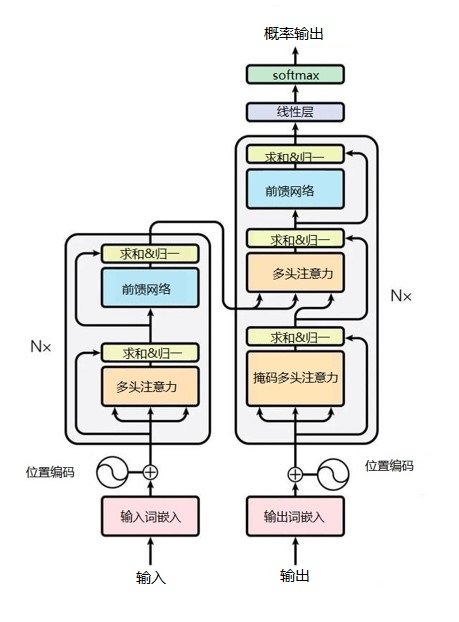
\includegraphics[scale = 0.8]{figures/Transformer2}
	\caption{Transformer 模型结构 \cite{transformer}}
	\label{fig:Transformer2}
\end{figure}

% \subsection{编码器-解码器结构}

(1) 编码器

编码器由 \(N=6\) 个相同的 TransformerEncoderLayer 层构成。每个 TransformerEncoderLayer 层可以再细分为两个子层。在这两个子层中,第一个子层实现了多头自注意力机制,而第二个子层则是一个简单的全连接前馈网络。每个子层后均接有残差连接,随后对经过残差连接的输出进行层归一化。为了确保残差连接的维度相等并便于计算,模型中所有子层及嵌入层的输出向量均设定为 \(d_{\text{model}} = 512\)。

(2) 解码器

解码器同样由 \(N=6\) 个相同的 TransformerDecoderLayer 层组成。每个 TransformerDecoderLayer 层包含三个子层。编码器层中的子层与在解码器其中两个子层的结构大致相似。但是在解码器层中,第三个子层需要获取编码器的输出及解码器层前一个子层的输出,并在该子层内执行多头注意力操作。与编码器层的子层结构相似,解码器层的每个子层后也接有残差连接,随后对经过残差连接的输出向量进行层归一化。Transformer 也将修改放入解码器结构中的自注意力子层中,加入了位置掩码,以防止从前面某个位置获取后面位置的信息。此位置掩码结合位置偏移的设计,确保序列中位置 \(i\) 的元素的预测仅能基于序列中小于 \(i\) 的所有内容。

% \subsection{注意力机制}

% 在 Transformer 中,定义注意力函数为输入为查询和一组键值,然后进行输出的函数,在此之中查询(Query, Q)、键(Key, K)、值(Value, V)和输出都是向量。在注意力函数中,简单地讲,输出实质上是值的加权和。此其中对于每个值的权重由权重相应的键以及查询计算得出。

% (1) 缩放点积注意力

% 在 Transformer 论文中所采用的注意力机制为缩放点积注意力。该机制的输入由查询、键和值组成,其中查询和键的维度均为 \(d_k\),而值的维度为 \(d_v\)。在缩放点积注意力中,我们首先计算查询与所有键向量之间的点积,并随后将这些结果除以 \(\sqrt{d_k}\)。接着,通过 softmax 函数对这些归一化后的向量进行处理,以计算每个值的权重。具体的过程如图 \ref{fig:DotAtt} 所示。

% \begin{figure}[htbp]
% 	\centering
% 	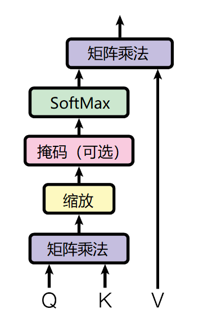
\includegraphics[scale = 0.8]{figures/DotAtt}
% 	\caption{缩放点积注意力 \cite{transformer}}
% 	\label{fig:DotAtt}
% \end{figure}

% 在实际应用中,对于一组待处理的注意力查询,应将这些查询同时进行计算,并将其封装为一个矩阵 \(Q\)。类似地,键和值也被封装为矩阵 \(K\) 和 \(V\)。通过这种方式,计算过程可以通过矩阵乘法进行优化。因此,注意力函数的输出矩阵可以表示为:
% \begin{equation}
% \text{Attention}(Q,K,V) = \text{softmax}(\frac{QK^T}{\sqrt{d_k}})V
% \label{eq3.1}
% \end{equation}

% (2) 多头注意力

% 实际上,如果将键、值和查询统一设定为 \(d_{\text{model}}\) 维度,反而可能导致模型性能下降,相较于将查询、键和值分别投影至 \(d_k\)、\(d_k\) 和 \(d_v\) 维度进行不同的线性变换。在此基础上,注意力函数在每个查询、键和值的投影向量上并行执行,从而生成 \(d_v\) 维的输出值。随后,将这些 \(d_v\) 维的输出值进行连接,并再次进行线性投影,以生成最终输出。具体过程如图 \ref{fig:MultiheadAtt} 所示。

% \begin{figure}[htbp]
% 	\centering
% 	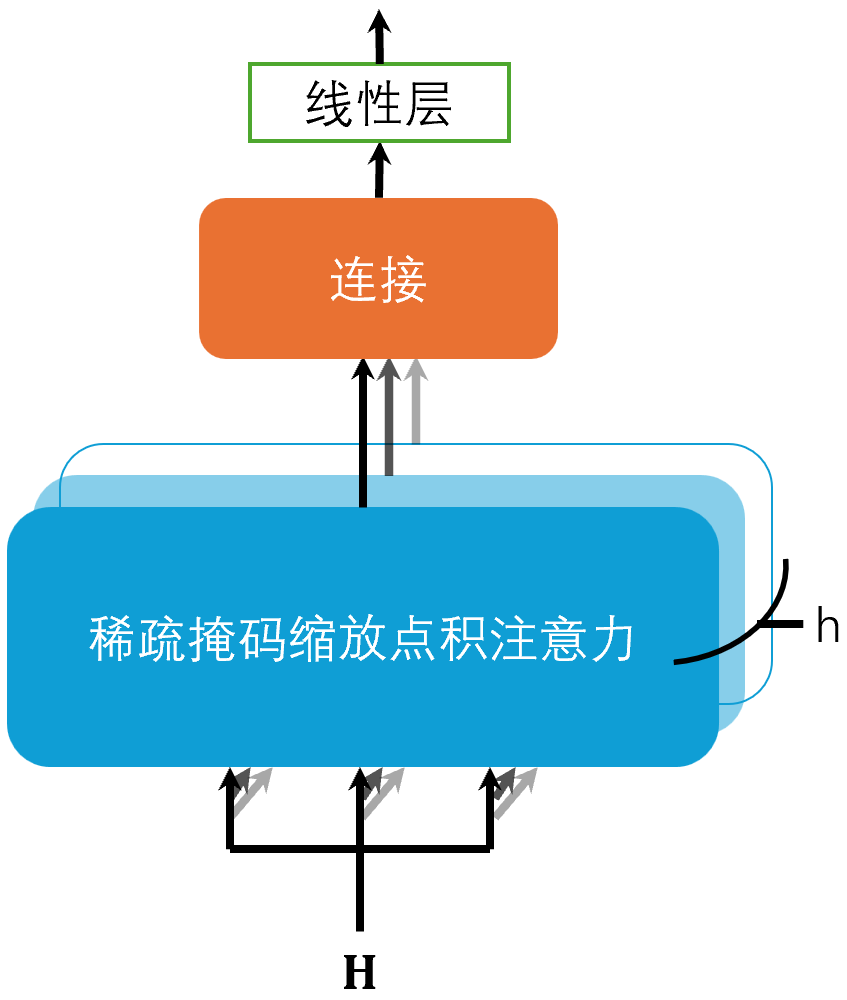
\includegraphics[scale = 0.8]{figures/MultiheadAtt}
% 	\caption{多头注意力 \cite{transformer}}
% 	\label{fig:MultiheadAtt}
% \end{figure}

% 多头注意力的主要优势在于其能够同时关注来自不同位置的信息。相较之下,单一注意力头的使用会导致信息的平均化,从而抑制这一特性。
% \begin{equation}
% \text{MultiHead}(Q, K, V) = \text{Concat}(\text{head}_1, ..., \text{head}_h)W^O
% \label{eq3.2}
% \end{equation}
% \begin{equation}
% \text{head}_i = \text{Attention}(QW_i^Q, KW_i^K, VW_i^V)
% \label{eq3.3}
% \end{equation}
% 在上述公式中,投影操作涉及的参数矩阵包括 \(W_i^Q \in \mathbb{R}^{d_{\text{model}}}\)、\(W_i^K \in \mathbb{R}^{d_{\text{model}} \times d_k}\)、\(W_i^V \in \mathbb{R}^{d_{\text{model}} \times d_v}\) 以及 \(W^O \in \mathbb{R}^{hd_v \times d_{\text{model}}}\)。

% 在 Transformer 架构中,采用了 \(h = 8\) 个并行的注意力层或头。对于每个注意力头,设定其维度为 \(d_k = d_v = d_{\text{model}} / h = 64\)。由于每个头的维度被缩减,因此整体计算成本与具有全维度的单头注意力相当。

% \subsection{位置前馈网络}

% 除了注意力子层外,编码器和解码器的每一层均包含一个全连接的前馈网络,该网络在每个位置上均以相同方式应用。该网络包括两个线性变换,并在其间引入一个线性整流单元(ReLU)激活函数。具体表达式为:
% \begin{equation}
% \text{FFN}(x) = \max(0, xW_1 + b_1)W_2 + b_2
% \label{eq3.4}
% \end{equation}

% 尽管在不同位置上应用的线性变换相同,但在层与层之间所使用的参数却是各异的。可以将其视作两个内核大小为 \(1\) 的卷积操作。输入和输出的维度均为 \(d_{\text{model}} = 512\),而内部层的维度为 \(d_{ff} = 2048\)。

% \subsection{嵌入层与 Softmax 函数}

% 与其他序列转换模型相似,Transformer 采用学习嵌入技术,将输入序列和输出序列中的词汇映射为维度为 \(d_{\text{model}}\) 的向量。此外,模型还利用常规的学习线性变换及 Softmax 函数,将解码器的输出转化为对下一个词汇的预测概率。在我们的模型中,两个嵌入层与预 Softmax 线性变换之间共享相同的权重矩阵。在嵌入层中,这些权重会乘以因子 \(\sqrt{d_{\text{model}}}\)。此外,也存在将 log-softmax 函数替代 Softmax 函数的做法。

% \subsection{位置编码}

% 由于 Transformer 模型不采用递归或卷积结构,为了使模型能够有效利用序列的顺序信息,必须引入某种形式的标记在序列中相对或绝对位置的信息。因此,我们在编码器和解码器堆栈的输入嵌入中添加了“位置编码”。位置编码的维度与嵌入相同,即 \(d_{\text{model}}\),从而可以将两者直接相加。位置编码的形式多种多样,既可以通过模型学习得到,也可以通过预定义的公式计算得出。

% 在 Transformer 中,采用了不同频率的正弦和余弦函数来生成位置编码,具体表达式为:
% \begin{equation}
% \begin{aligned}
% \text{PE}(pos,2i) &= \sin \left ( \frac{pos}{10000^{2i/d_{\text{model}}}} \right ) \\
% \text{PE}(pos,2i+1) &= \cos \left ( \frac{pos}{10000^{2i/d_{\text{model}}}} \right )
% \end{aligned}
% \label{eq3.5}
% \end{equation}
% 其中 \(pos\) 表示位置,\(i\) 表示维度。换言之,位置编码的每个维度对应于一条正弦曲线,其波长形成从 \(2\pi\) 到 \(10000 \cdot 2\pi\) 的几何级数。选择这种函数的原因在于我们假设它能够使模型更容易地学习通过相对位置进行计算,因为对于任何固定的偏移量 \(k\),\(\text{PE}_{pos+k}\) 可以表示为 \(\text{PE}_{pos}\) 的线性函数。

% \subsection{线性层}

% 在数据经过 log-softmax 函数处理后,将通过一层线性层将维度为 \(d_{\text{model}}\) 的向量转换为一个维度等于词汇表大小的向量,该向量用于表示对下一个预测词汇的概率分布。

\section{预训练语言模型技术}

近年来,自然语言处理(Natural Language Processing, NLP)领域经历了显著的进展,其中预训练语言模型(Pre-trained Language Models, PLMs)的研究为该领域的发展提供了重要支持。预训练语言模型的核心思想是首先在进行预训练阶段的训练,基于大规模数据集的训练以获得模型参数,此举可使模型获得对于数据初步的认知,随后利用这些经过训练的模型来在具体的下游任务数据上进行微调。预训练语言模型的早期研究甚至可以追溯到 NNLM \cite{NNLM} 和 word2Vec \cite{mikolov2013efficientestimationwordrepresentations}。2017 年,Vaswani 等人 \cite{transformer} 提出了 Transformer 架构,这一架构的引入显著提升了多种 NLP 任务的性能,使 Transformer 成为众多预训练语言模型的基础。在基于 Transformer 的编码器架构中,Radford 等人 \cite{gpt} 提出了 GPT 模型,该模型真正实现了预训练-微调的框架,避免了将词嵌入从模型中提取的过程。目前,GPT 模型的应用取得了显著成功,各种大型 GPT 模型层出不穷,为 NLP 等领域注入了新的活力。同时,Devlin 等人 \cite{devlin_bert_2019} 基于 Transformer 的编码器提出了 BERT 模型,成为目前自然语言处理领域中应用最广泛的模型之一。BERT 在预训练阶段,采用了掩码语言模型(Masked Language Model, MLM)的方法。这种方法是从输入文本中通过随机掩盖某些词元,此后利用除了被掩盖词元外的上下文信息进行预测,从而实现对模型的训练。继 GPT 和 BERT 之后,研究人员还提出了 XLNet \cite{XLNet}、RoBERTa \cite{liu_roberta_2019}、DeBERTa \cite{he_deberta_2021}、ERNIE \cite{sun2019ernieenhancedrepresentationknowledge}、T5 \cite{T5} 和 BART \cite{lewis-etal-2020-bart} 等多种预训练语言模型。本节将介绍本文所采用的 RoBERTa 和 DeBERTa 模型的基础预训练语言模型 BERT 模型。

% 写写 BERT 吧
BERT(Bidirectional Encoder Representations from Transformers)\cite{devlin_bert_2019} 是由 Google 提出的预训练模型。该模型在机器阅读理解的顶级基准测试 SQuAD1.1 \cite{rajpurkar2016squad100000questionsmachine} 中展现了卓越的性能:在所有两个评估指标上均显著超越了人类表现,并在 11 项不同的 NLP 测试中创造了最新的状态-of-the-art(SOTA)成绩。其中,GLUE 基准 \cite{wang2019gluemultitaskbenchmarkanalysis} 的得分提升至 80.4\%(绝对改进 7.6\%),而 MultiNLI 数据集 \cite{williams2018broadcoveragechallengecorpussentencemultinli} 的准确率达到 86.7\%(绝对改进 5.6\%),标志着这一模型在自然语言处理领域的里程碑式成就。BERT 在 Transformer 架构的基础上引入了预训练与微调的策略,使得模型能够在预训练阶段学习通用的语言表示,并在特定任务中进行微调,从而显著提高了模型的适应性与性能。因此,尽管 BERT 并非首个预训练模型,但在预训练模型的发展历程中,其重要性不容忽视,具有里程碑式的意义。

\subsection{BERT 结构}

BERT 在 Transformer 的基础上并未进行大量改进,而是采用了 Transformer 编码器的结构作为其核心架构。其总体结构如图 \ref{fig:BERT} 所示,多个 Transformer 编码器层逐层堆叠构成了 BERT 的整体框架。在原始论文中,作者分别构建了两种 BERT 模型,采用了 12 层和 24 层的 Transformer 编码器,分别对应于 110M 和 340M 的总参数量。

\begin{figure}[htb]
	\centering
	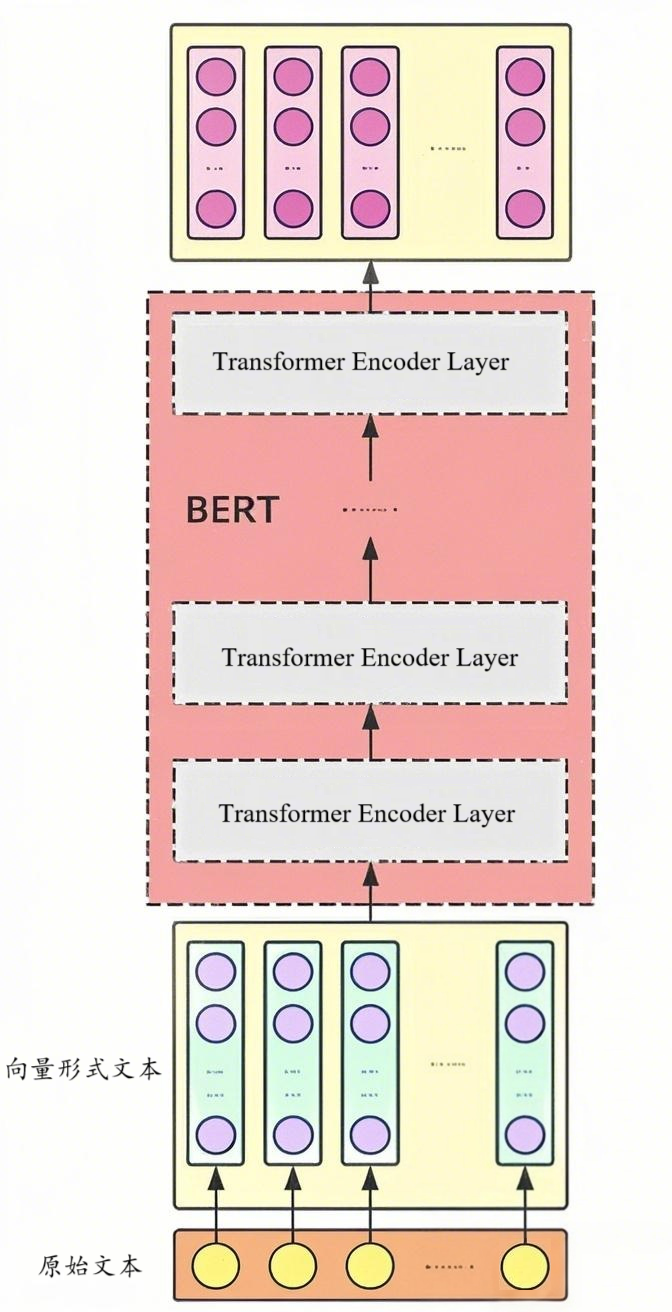
\includegraphics[scale = 0.5]{figures/bert.png}
	\caption{BERT 架构图 \cite{devlin_bert_2019}}
	\label{fig:BERT}
\end{figure}

\subsubsection{嵌入}

对于 BERT 而言,其在嵌入(Embedding)方面的显著改进是一个关键创新。为了使 BERT 能够有效处理多种下游任务,其输入表示能够清晰地区分单个句子和句子对(例如,〈问题, 答案〉)在同一词元序列中。

在 BERT 中,每个序列的首个词元始终是一个特殊的非正文的分类词元([CLS]),该标记的最终向量可视为整句话的语义表示,进而用于下游的分类任务等。由于该标记本身并非正文内容,因此缺乏明显的语义信息,使用它的最终向量能恰好地在文本中整合各个词的语义。在经过 BERT 这一预训练语言模型的处理后,所有词的信息同时也被融合进入了每个词的嵌入中,从而更准确地反映其语义。在 BERT 的执行过程中,句子对会被合并成一个序列然后由 BERT 模型处理。区分句子大致分为两步。首先,在原始输入文本中加入特殊标记([SEP])分开两个句子。其次,BERT 将句子嵌入融合到每个词元生成的向量中,以表明其为哪个句子。

\begin{figure}[htb]
	\centering
	\includegraphics[width=0.9\linewidth]{figures/bert_Input_Embeddings.jpg}
	\caption{BERT 嵌入(Embedding)示意图 \cite{devlin_bert_2019}}
	\label{fig:BERT-embedding}
\end{figure}

对于每个给定的词元,其输入表示(input representation)是通过对相应的词元(token)、段落(segment)和位置(position)嵌入进行加和来构建的。该结构的可视化展示见图 \ref{fig:BERT-embedding}。

\subsubsection{预训练与微调}

BERT 研究的主要贡献在于其二阶段训练过程的有效推广,该过程分为预训练(pretraining)和微调(finetuning)两个阶段,训练流程的示意图如图 \ref{fig:BERT-OverAll} 所示。在预训练阶段,BERT 通过大规模的无标注文本数据学习语言的深层次表示,采用了带掩码的语言模型(Masked Language Model, MLM)和下一句预测(Next Sentence Prediction, NSP)两种任务,从而使模型能够理解上下文的双向信息。在微调阶段,BERT 通过在少量标注数据上进行训练,能够针对特定任务进行调整,进而高效适应多种自然语言处理任务,如文本分类、问答系统和命名实体识别等。

\begin{figure}[htb]
	\centering
	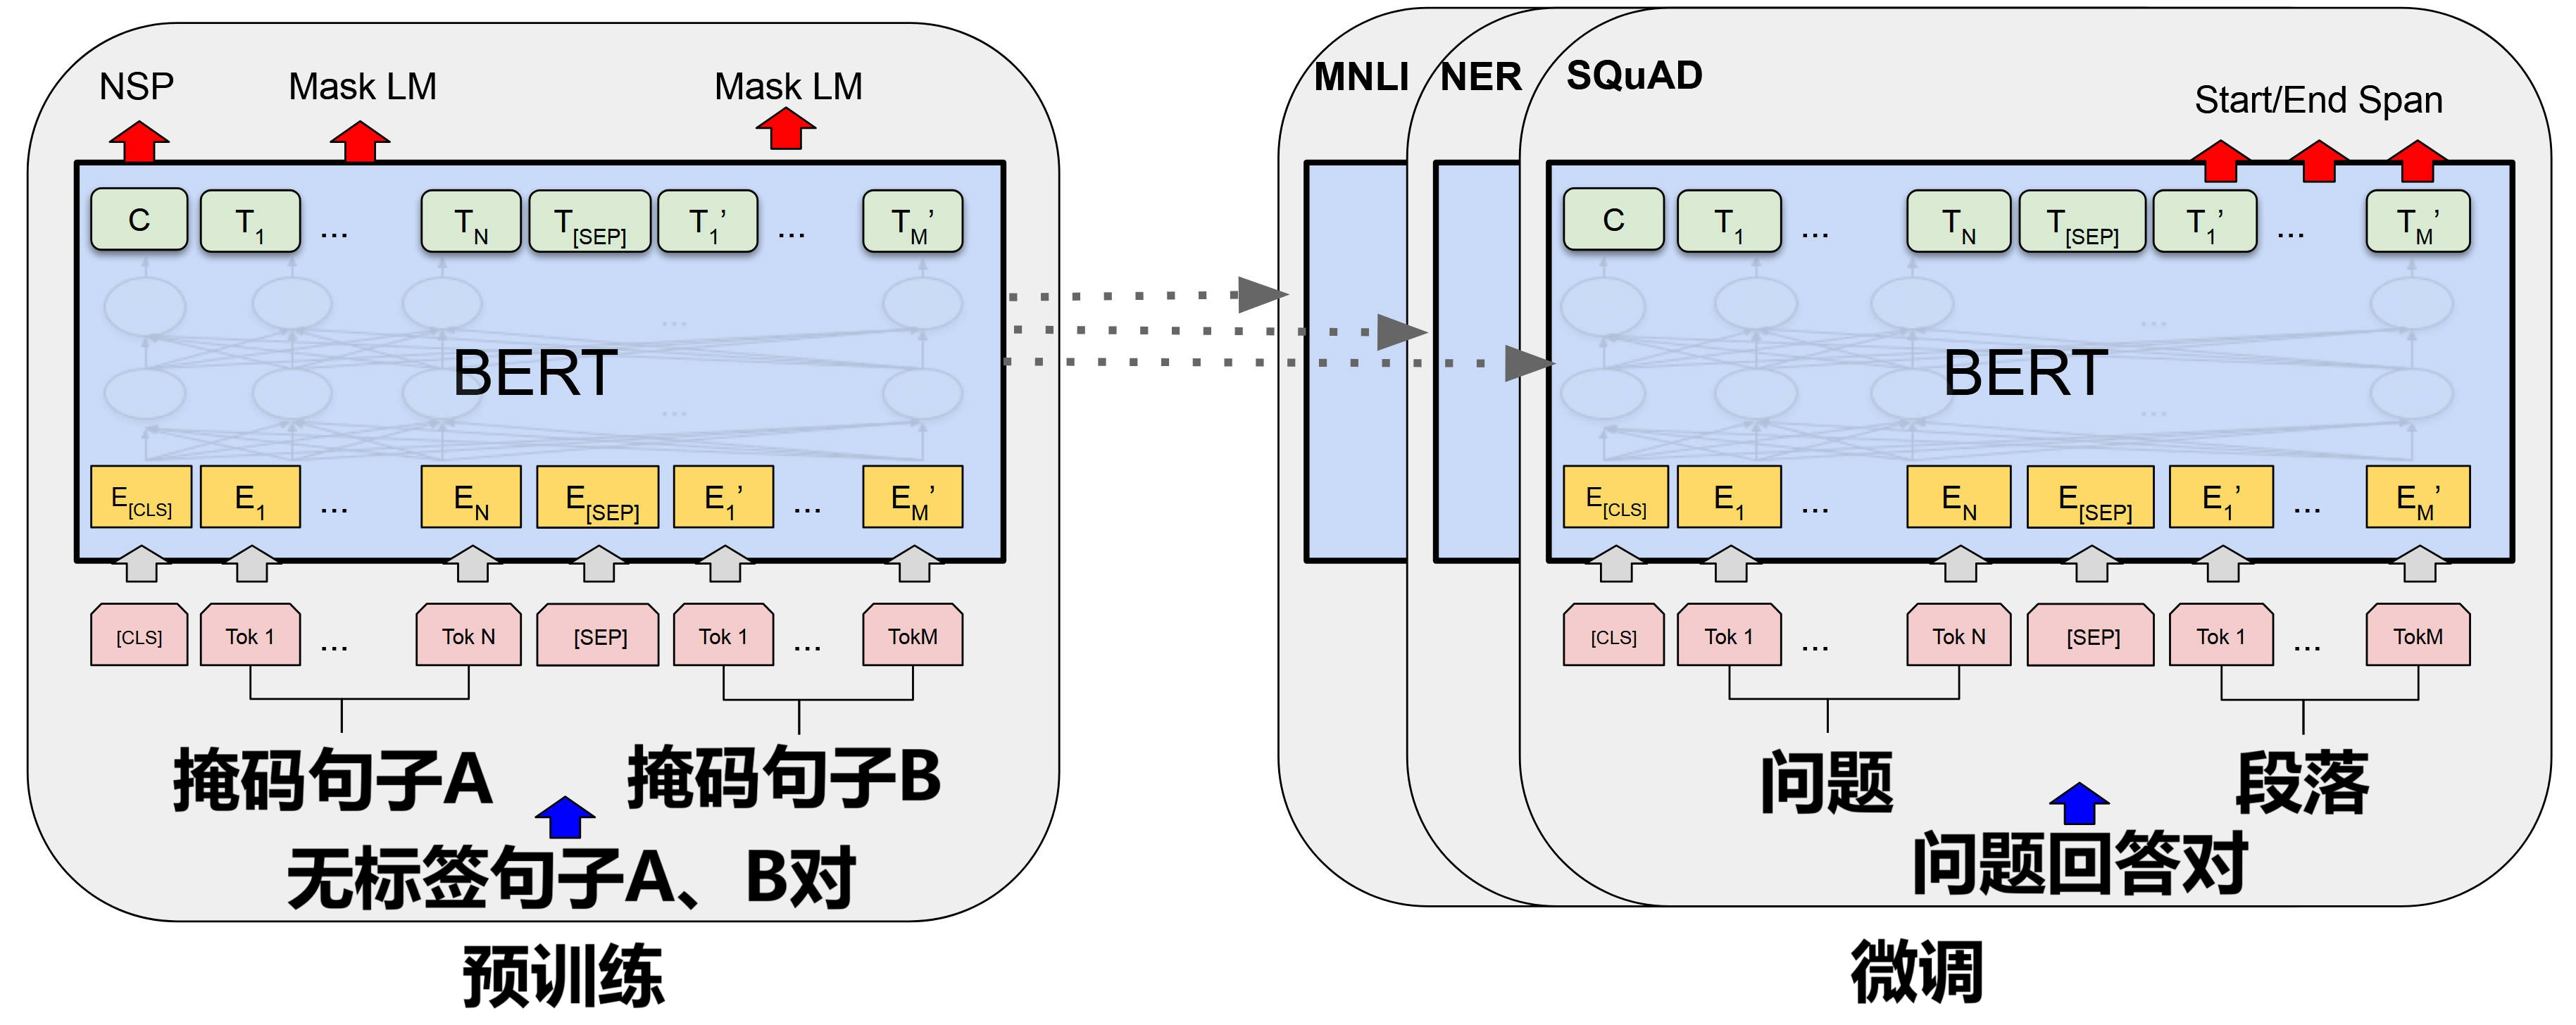
\includegraphics[width=0.9\linewidth]{figures/BERT_Overall.jpg}
	\caption{BERT 训练过程示意图 \cite{devlin_bert_2019}}
	\label{fig:BERT-OverAll}
\end{figure}

这种预训练-微调的二阶段训练范式显著提高了模型在多种自然语言处理(NLP)任务上的性能,标志着该领域的一次重要变革。BERT 的成功激励了大量基于 Transformer 架构的预训练模型的后续研发,例如本文将使用的 RoBERTa 和 DeBERTa,以及其他在 BERT 模型基础上进行改进的模型。这些模型在不同任务中展现出更高的效率和准确性。通过这些创新,BERT 不仅推动了学术界对预训练模型的深入研究,也促进了工业界在实际应用中的广泛采用。

\subsection{RoBERTa 模型}
\label{sec:method-pretrain-roberta}

RoBERTa \cite{liu_roberta_2019}(Robustly Optimized BERT Approach)在 BERT \cite{devlin_bert_2019} 模型的基础上进行了多方面的优化,显著提升了模型的整体性能。

在训练策略方面,原始 BERT 模型存在训练不足的问题。为了解决这一缺陷,RoBERTa 通过延长训练步数、采用更大的批次进行训练,并在更广泛的数据集上进行训练。在实验中,较大的批次训练 BERT 模型的结果表明,这种策略能够有效降低训练的困惑度(perplexity),并提高下游任务的准确率。此外,大批次训练更易于通过分布式数据并行实现,从而显著提升了训练效率。

在训练数据的选择上,RoBERTa 使用了总计 160GB 的未压缩文本,涵盖多种语料库,这一数据量远超 BERT 原始训练所用的 16GB。此结果充分表明数据量和多样性在预训练过程中的重要性。此外,BERT 原始实现中,掩码是在数据预处理阶段一次性生成的,形成了静态掩码。尽管通过数据复制增加掩码的多样性,但该方法仍存在局限性。相较之下,RoBERTa 采用了动态掩码机制,即在每次向模型输入序列时生成新的掩码模式。这一方法在长时间训练或处理大规模数据集时表现出明显优势,不仅提高了训练效率,还在实验中显示出相较于静态掩码更优或相当的性能。

在模型输入格式的优化方面,原始 BERT 模型在训练时使用了下一个句子预测(NSP)任务,以提升下游任务的性能。然而,相关研究 \cite{Lample2019CrosslingualLM, Yang2019XLNetGA, Joshi2019SpanBERTIP} 对这一任务提出了质疑。RoBERTa 经过对比实验发现,去除 NSP 损失并采用从单个文档中采样完整句子作为输入,能够匹配或略微提升下游任务的性能。具体而言,限制序列来自单个文档的 DOC-SENTENCES 格式表现优于从多个文档打包的 FULL-SENTENCES 格式,但为了便于与相关研究的比较,最终 RoBERTa 选择了从多个文档打包的 FULL-SENTENCES 格式。此外,RoBERTa 不再使用 BERT 原有的两文档片段拼接并添加 NSP 损失的输入格式,而是采用从一个或多个文档中连续采样完整句子的方式,确保输入总长度不超过 512 个标记。这一格式有助于模型学习长距离依赖关系,从而增强文本理解能力。

在文本编码的改进方面,BERT 原实现使用了一个大小为 30K 的字符级字节对编码 \cite{BPE}(BPE)词汇表,并需要进行启发式分词规则的预处理。RoBERTa 借鉴其他研究,采用了一个包含 50K 子词单元的更大字节级 BPE 词汇表,这一方法无需额外的预处理或分词。尽管在某些任务上性能略有下降,但由于其通用编码方案的优势,RoBERTa 仍被广泛应用于后续的实验中。

通过以上对 BERT 的改进,RoBERTa 在多个自然语言处理任务中展现出卓越的性能,为后续研究提供了强有力的支持。

在本文中,采用 RoBERTa-base 和 RoBERTa-Large 两种大小的 RoBERTa 模型,其参数如表 \ref{tab:roberta-parameter} 所示。表中的参数包括 Transformer 层数、隐藏层维度、注意力头数以及总参数量。这些参数的设计反映了模型的复杂性及其学习能力。较大的模型(RoBERTa-Large)在处理更复杂的语言任务时,能够更好地捕捉深层次的语义关系和上下文信息,而较小的模型(RoBERTa-Base)则在计算效率和资源消耗上具有一定的优势。通过对比这两种模型的性能,我们能够深入探讨不同规模模型在文本理解和生成任务中的表现差异,从而为后续研究提供有价值的参考。

\begin{table*}[htbp]
\centering
\caption{ RoBERTa-Base 和 RoBERTa-Large 参数} \label{tab:roberta-parameter}
\begin{tabular}{lcc}
\toprule
               & \multicolumn{1}{l}{\textbf{RoBERTa-Base} \cite{liu_roberta_2019}} & \multicolumn{1}{l}{\textbf{RoBERTa-Large} \cite{liu_roberta_2019}} \\ \midrule
Transformer 层数 & 12                                        & 24                                         \\
隐藏层维度          & 768                                       & 1024                                       \\
注意力头数          & 12                                        & 16                                         \\
总参数量           & 125M                                      & 355M                                      \\ \bottomrule
\end{tabular}
\end{table*}

\subsection{DeBERTa 模型}
\label{sec:method-pretrain-deberta}

目前 DeBERTa 系列模型公开的论文仅有 DeBERTa 模型 \cite{he_deberta_2021} 和 DeBERTa V3 模型 \cite{he2023debertav3improvingdebertausing},我们的实验中将会使用 DeBERTa V3 模型,本节将会对 DeBERTa 模型对于 BERT \cite{devlin_bert_2019} 和 RoBERTa 模型 \cite{liu_roberta_2019} 的改进进行介绍。

\subsubsection{DeBERTa 模型}

DeBERTa 模型 \cite{he_deberta_2021} 是预训练语言模型演进过程中的一项重要成果,相较于本文先前提及的 RoBERTa 和 BERT,其在多个方面进行了显著改进。这些改进主要体现在注意力机制、掩码解码器以及训练方法等方面,从而显著提升了模型的性能和泛化能力。

在注意力机制的设计上,BERT 和 RoBERTa 将每个单词表示为其词嵌入(内容)与位置嵌入的和,这种表示方式在一定程度上融合了内容和位置信息。相较之下,DeBERTa 采用了一种创新的解耦注意力机制,将每个单词分别编码为两个独立的向量,分别代表内容和位置。在计算单词间的注意力权重时,DeBERTa 利用基于内容和相对位置的解耦矩阵进行独立计算。这种方法使得模型能够更精细地捕捉单词之间的关系。以句子 “The dog chased the cat” 为例,当分析 “dog” 与 “cat” 之间的关系时,DeBERTa 不仅考虑它们的语义内容,还能基于相对位置更准确地判断其依赖关系。相较而言,BERT 和 RoBERTa 在处理这种复杂关系时则显得不够细致。

对于序列中位置为 \(i\) 的词元(token),DeBERTa 采用两个向量进行表示,分别为 \(\mathbf{H}_{i}\) 和 \(\mathbf{P}_{i|j}\)。其中,\(\mathbf{H}_{i}\) 表示该词元的内容信息,而 \(\mathbf{P}_{i|j}\) 则表示该词元与位置为 \(j\) 的词元之间的相对位置关系。词元 \(i\) 与 \(j\) 之间的交叉注意力分数的计算可以被分解为四个组成部分,具体如下:
\begin{align}
\label{eq:deberta-attention}
\begin{split}
\mathbf{A}_{i, j} & = \{\mathbf{H}_{i}, \mathbf{P}_{i | j}\} \times \{\mathbf{H}_{j}, \mathbf{P}_{j | i}\}^{\intercal} \\
& = \mathbf{H}_{i}\mathbf{H}_{j}^{\intercal}+\mathbf{H}_{i}\mathbf{P}_{j | i}^{\intercal}+\mathbf{P}_{i | j}\mathbf{H}_{j}^{\intercal}+\mathbf{P}_{i | j}\mathbf{P}_{j | i}^{\intercal}.
\end{split}
\end{align}

换言之,单词对之间的注意力权重可以通过将基于其内容和位置的解耦矩阵应用于四个注意力分数的求和来计算。这四个分数分别对应于内容对内容、内容对位置、位置对内容以及位置对位置的注意力。

在 DeBERTa 之前,相对位置编码的方法在计算注意力权重时,通常依赖于独立的嵌入矩阵来确定相对位置偏差 \cite{Shaw2018SelfAttentionWR, Huang2018MusicTG}。这相当于仅利用公式 \ref{eq:deberta-attention} 中的内容对内容和内容对位置这两项计算注意力权重。因为单词对的注意力权重不仅依赖于其内容信息,还受到相对位置的影响,因此位置对内容的项同样十分重要。由于在 DeBERTa 中处理位置的方式是相对位置嵌入,因此位置对位置的该项在 DeBERTa 的中被认为提供的额外信息有限,因此从公式 \ref{eq:deberta-attention} 中去除了该项。

以单头注意力为例,标准的自注意力操作 \cite{transformer} 可以表示为:
\begin{align}
\mathbf{Q} = \mathbf{HW_{q}}, \mathbf{K} &= \mathbf{HW_{k}}, V = \mathbf{HW_{v}}, \mathbf{A} = \frac{\mathbf{QK}^{\intercal}}{\sqrt{d}} \\
\mathbf{H_{o}} &= \text{softmax}(\mathbf{A})\mathbf{V}
\label{eq:transformer-attention1}
\end{align}
其中,$\mathbf{H} \in \mathbb{R}^{N×d}$ 表示输入的隐藏向量,$\mathbf{H_{o}} \in \mathbb{R}^{N×d}$ 是自注意力的输出,$\mathbf{W_{q}}$、$\mathbf{W_{k}}$、$\mathbf{W_{v}} \in \mathbb{R}^{d×d}$ 是投影矩阵,$\mathbf{A} \in \mathbb{R}^{N×N}$ 是注意力矩阵,$N$ 是输入序列的长度,$d$ 是隐藏状态的维度。

记 $k$ 为最大相对距离,$\delta(i, j) \in [0, 2k)$ 为从词元 $i$ 到词元 $j$ 的相对距离,其定义为:
\begin{align}
\delta(i, j)=\begin{cases}
0, & \text{当~} i - j \leq -k \\
2k - 1, & \text{当~} i - j \geq k \\
i - j + k, & \text{其他情况}
\end{cases}
\label{eq:deberta-distance}
\end{align}

在 DeBERTa 中,带有相对位置偏差的解耦自注意力机制可以用公式 \ref{eq:deberta-dis-att} 来表示。在该公式中,\(\mathbf{Q}_{c}\)、\(\mathbf{K}_{c}\) 和 \(\mathbf{V}_{c}\) 分别是通过投影矩阵 \(\mathbf{W}_{q,c}\)、\(\mathbf{W}_{k,c}\) 和 \(\mathbf{W}_{v,c} \in \mathbb{R}^{d \times d}\) 生成的投影内容向量。此外,\(\mathbf{P} \in \mathbb{R}^{2k \times d}\) 表示在所有层中共享的相对位置嵌入向量,该向量在正向传播过程中保持不变。相对位置向量 \(\mathbf{Q}_{r}\) 和 \(\mathbf{K}_{r}\) 则是通过投影矩阵 \(\mathbf{W}_{q,r}\) 和 \(\mathbf{W}_{k,r} \in \mathbb{R}^{d \times d}\) 生成的。
\begin{align} \label{eq:deberta-dis-att}
\begin{split}
    \mathbf{Q}_c = \mathbf{H} \mathbf{W}_{q,c}, 
    \mathbf{K}_c &= \mathbf{H} \mathbf{W}_{k,c}, 
    \mathbf{V}_c = \mathbf{H} \mathbf{W}_{v,c}, 
    \mathbf{Q}_r = \mathbf{P} \mathbf{W}_{q,r}, 
    \mathbf{K}_r = \mathbf{P} \mathbf{W}_{k,r} \\
    \tilde{\mathbf{A}}_{i,j} &= \underbrace{\mathbf{Q}^{c}_{i}{\mathbf{K}^{c}_{j}}^{\intercal}}_{\text{(a) content-to-content}}  
    + \underbrace{\mathbf{Q}^{c}_{i}{{\mathbf{K}^{r}_{\delta(i,j)}}^{\intercal}}}_{\text{(b) content-to-position}}
    + \underbrace{\mathbf{K}^{c}_{j}{{\mathbf{Q}^{r}_{\delta(j,i)}}^{\intercal}}}_{\text{(c) position-to-content}} \\
    \mathbf{H_o} &= \text{softmax}(\frac{\tilde{\mathbf{A}}}{\sqrt{3d}})\mathbf{V}_c
\end{split}
\end{align}
在此,\(\tilde{\mathbf{A}}_{i,j}\) 表示注意力矩阵 \(\tilde{\mathbf{A}}\) 的一个元素,具体对应于词元 \(i\) 到词元 \(j\) 的注意力分数。具体而言,\(\mathbf{Q}_{i}^{c}\) 是矩阵 \(\mathbf{Q}_{c}\) 的第 \(i\) 行,而 \(\mathbf{K}_{j}^{c}\) 则是矩阵 \(\mathbf{K}_{c}\) 的第 \(j\) 行。同时,\(\mathbf{K}_{\delta(i,j)}^{r}\) 表示相对位置向量 \(\mathbf{K}_{r}\) 中与相对距离 \(\delta(i,j)\) 对应的第 \(\delta(i,j)\) 行,\(\mathbf{Q}_{\delta(j,i)}^{r}\) 则是与相对距离 \(\delta(j,i)\) 对应的第 \(\delta(j,i)\) 行。值得注意的是,DeBERTa 在此使用 \(\delta(j,i)\) 而非 \(\delta(i,j)\),原因在于对于特定位置 \(i\),位置对内容的计算实际上是基于位置 \(j\) 的键内容相对于位置 \(i\) 的查询位置的注意力权重。因此,此时相对距离应为 \(\delta(j,i)\)。位置对内容项的计算公式为 \(\mathbf{K}_{j}^{c} \cdot {\mathbf{Q}_{\delta(j,i)}^{r}}^{\intercal}\),而内容对位置的计算方式则类似。

最后,对注意力矩阵 \(\tilde{\mathbf{A}}\) 应用一个缩放因子 \(\frac{1}{\sqrt{3d}}\)。这一缩放因子在模型训练的稳定性方面发挥了关键作用 \cite{transformer},尤其是在处理大规模预训练语言模型时,其重要性愈加突出。

\begin{algorithm}[htb]
\caption{解耦注意力(Disentangled Attention)}
\label{algo:DA}
%\SetAlgoLined
 \begin{algorithmic}[1]
    \Require {隐藏状态 $\mathbf{H}$, 相对距离嵌入 $\mathbf{P}$, 相对距离矩阵 $\mathbf{\delta}$.}
    内容投影矩阵 $\mathbf{W}_{k,c}$, $\mathbf{W}_{q,c}$, $\mathbf{W}_{v,c}$,
    位置投影矩阵 $\mathbf{W}_{k,r}$, $\mathbf{W}_{q,r}$.
    \Ensure $\mathbf{H}_o$

    \State {$\mathbf{K}_c = \mathbf{H}\mathbf{W}_{k,c}$, $\mathbf{Q}_c = \mathbf{H}\mathbf{W}_{q,c}$, $\mathbf{V}_c = \mathbf{H}\mathbf{W}_{v,c}$,   $\mathbf{K}_r = \mathbf{P}\mathbf{W}_{k,r}$, $\mathbf{Q}_r = \mathbf{P}\mathbf{W}_{q,r}$}
    \State {$\mathbf{A}_{c\rightarrow c} = \mathbf{Q}_c \mathbf{K}_c^{\intercal}$} 
    \For{$i=0,...,N-1$} 
        \State {$\tilde{\mathbf{A}}_{c\rightarrow p}[i,:] = \mathbf{Q}_{c}[i,:] \mathbf{K}_r^{\intercal}$} 
    \EndFor
    \For {$i=0,...,N-1$}
        \For {$j=0,...,N-1$}
        \State {$\mathbf{A}_{c\rightarrow p}[i,j] = \tilde{\mathbf{A}}_{c\rightarrow p}[i,\mathbf{\delta}[i,j]]$} 
        \EndFor
    \EndFor
    \For{$j=0,...,N-1$}
        \State {$\tilde{\mathbf{A}}_{p\rightarrow c}[:,j] = \mathbf{K}_{c}[j,:] \mathbf{Q}_r^{\intercal}$} 
    \EndFor
    \For {$j=0,...,N-1$}
        \For {$i=0,...,N-1$}
        \State {$\mathbf{A}_{p\rightarrow c}[i,j] = \tilde{\mathbf{A}}_{p\rightarrow c}[\mathbf{\delta}[j,i],j]$} 
        \EndFor
    \EndFor
    \State {$\tilde{\mathbf{A}}=\mathbf{A}_{c\rightarrow c} + \mathbf{A}_{c\rightarrow p} + \mathbf{A}_{p\rightarrow c}$}
    \State {$\mathbf{H}_o = \text{softmax}(\frac{\tilde{\mathbf{A}}}{\sqrt{3d}})\mathbf{V}_c$}
 \end{algorithmic}

\end{algorithm}

DeBERTa 采用了一种高效的实现方法。在其之前的研究中,对于长度为 \(N\) 的输入序列,每个词元的相对位置嵌入需要 \(O(N^{2}d)\) 的空间复杂度 \cite{Shaw2018SelfAttentionWR, Huang2018MusicTG, Dai2019TransformerXLAL}。然而,以内容对位置的计算为例,DeBERTa 观察到相对距离 \(\delta(i, j)\) 的范围为 \([0, 2k)\),并且所有可能的相对位置嵌入实际上构成了矩阵 \(\mathbf{K}_{r} \in \mathbb{R}^{2k \times d}\) 的一个子集。因此,我们能够在所有查询的注意力计算过程中重用 \(\mathbf{K}_{r}\),从而显著降低了存储需求。

在 DeBERTa 中,预训练阶段将最大相对距离 \(k\) 设置为 512。解耦的注意力权重可以通过算法 \ref{algo:DA} 高效计算。设 \(\delta\) 为根据公式 \ref{eq:deberta-distance} 得到的相对位置矩阵,其中 \(\delta[i, j] = \delta(i, j)\)。在此过程中,我们并不为每个查询分配独立的相对位置嵌入矩阵,而是通过将每个查询向量 \(\mathbf{Q}_{c}[i, :]\) 乘以 \(\mathbf{K}_{r}^{\intercal} \in \mathbb{R}^{d \times 2k}\)(如算法 \ref{algo:DA} 的第 3-5 行),并利用相对位置矩阵 \(\delta\) 作为索引来提取注意力权重(如算法 \ref{algo:DA} 的第 6-10 行)。为了计算位置对内容的注意力分数,我们通过将每个键向量 \(\mathbf{K}_{c}[j, :]\) 乘以 \(\mathbf{Q}_{r}^{T}\) 来获得注意力矩阵 \(\tilde{\mathbf{A}}_{p \to c}[:, j]\) 的列向量(如算法 \ref{eq:deberta-distance} 的第 11-13 行),并最终通过相对位置矩阵 \(\delta\) 作为索引提取相应的注意力分数(如算法 \ref{algo:DA} 的第 14-18 行)。通过这种方法,我们避免了为每个查询分配内存以存储相对位置嵌入,从而将空间复杂度降低至 \(O(kd)\),仅需存储 \(\mathbf{K}_{r}\) 和 \(\mathbf{Q}_{r}\)。

此外,DeBERTa 还采用了掩码语言建模(Masked Language Modeling, MLM)作为预训练策略。在这一过程中,模型通过利用周围未被掩码的词汇来预测被掩码的词。DeBERTa 在掩码语言模型任务中充分考虑了位置信息及其上下文词的内容。在解耦注意力机制,上下文词的内容和相对位置被提到了相当重要的位置,但这些词的绝对位置却并没有被该方法充分使用。多数情况下,精确预测高度依赖于绝对位置信息。

\begin{figure*}[htbp]
\centering  
\subfloat[BERT 解码层]{
    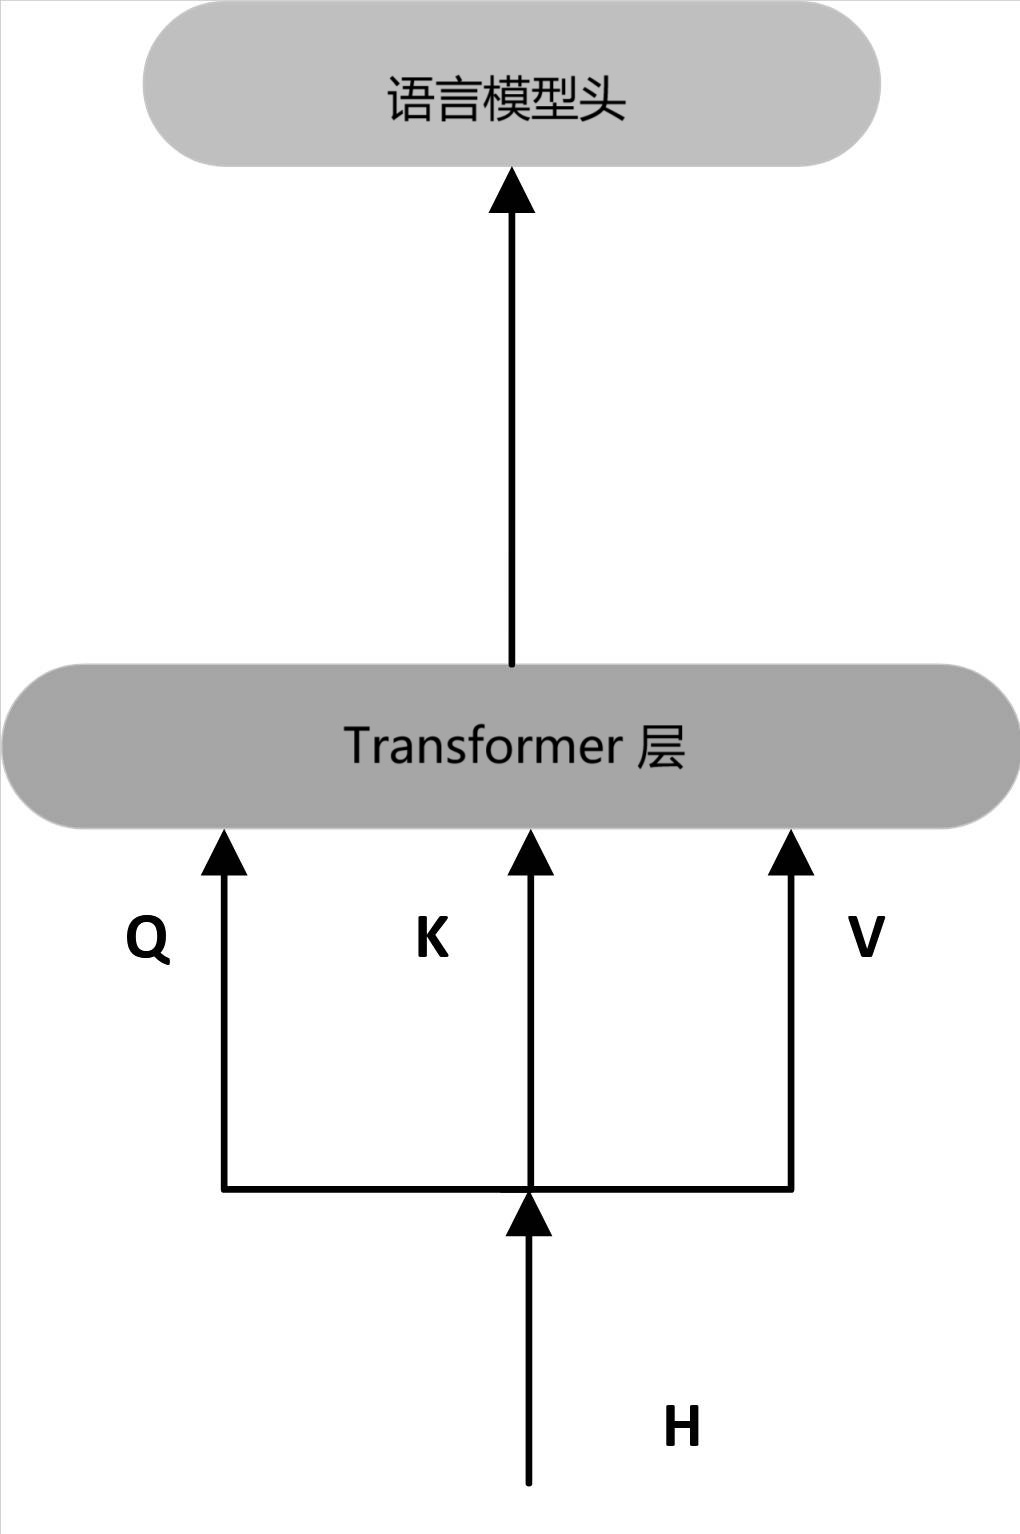
\includegraphics[trim={0.5mm 0.5mm 0.5mm 0.5mm},clip,width=0.35\linewidth]{figures/Model_BERT_S.jpg}
    % \label{fig:bert-a}
}
\hfill
\subfloat[改进的遮掩解码]{
    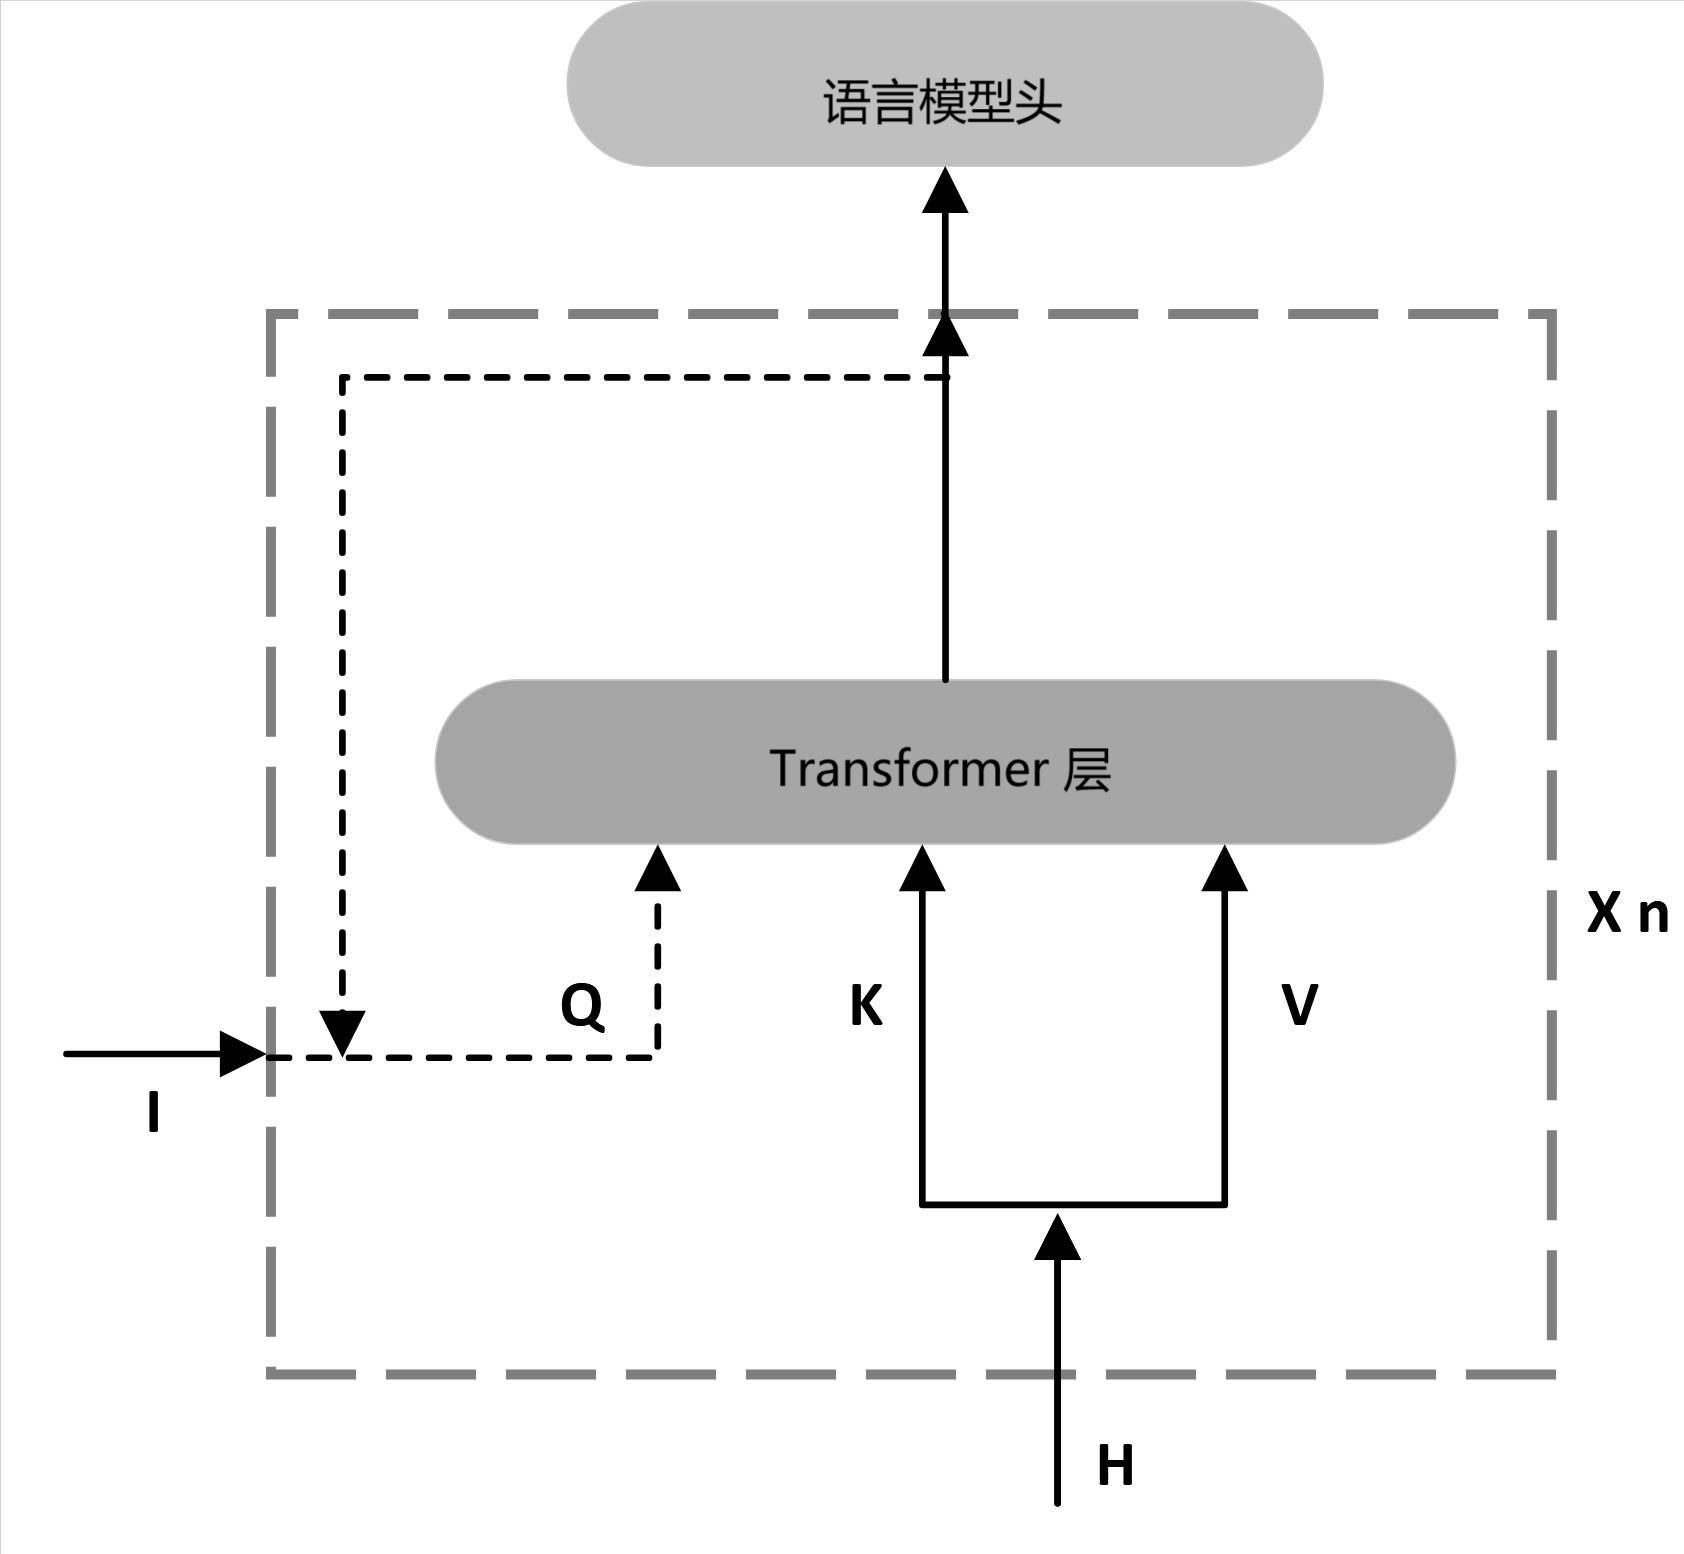
\includegraphics[trim={0.5mm 0.5mm 0.5mm 0.5mm},clip,width=0.58\linewidth]{figures/Model_EMD_S.jpg}
    % \label{fig:emd-b}
}

\caption{BERT 与 DeBERTa 解码层的比较 \cite{he_deberta_2021}}
\label{fig:emd}
\end{figure*}

将绝对位置信息整合到模型中可以通过两种主要方式实现。BERT 模型选择在输入层直接引入绝对位置信息。相较之下,DeBERTa 结构则在所有 Transformer 层之后、但在基于聚合的上下文词内容和位置嵌入解码掩码词的 Softmax 层之前,添加绝对位置信息,如图 \ref{fig:emd} 所示。这种创新架构使DeBERTa具备双重优势:一方面在全部Transformer层级中精准建模相对位置关系,另一方面在重构遮蔽标记时巧妙融合绝对位置特征作为辅助信号。正是基于这一独特机制,该模型将其核心解码模块命名为“增强型掩码解码器”(Enhanced Mask Decoder, EMD)。

\subsubsection{DeBERTa V3 模型}

由于 ELECTRA \cite{clark2020electrapretrainingtextencoders} 中的替换词元检测(Replaced Token Detection, RTD)和 DeBERTa 中的解耦注意力机制已被证实在预训练阶段具有较高的样本效率,DeBERTa V3 因而应运而生。该模型将原始 DeBERTa 中采用的掩码语言模型(Masked Language Modeling, MLM)目标替换为替换词元检测目标,以充分整合后者的优势。

基于 Transformer 的预训练语言模型通常在大规模文本数据集上进行训练,旨在通过自监督学习的目标来获取上下文中单词的表示,这一目标被称为掩码语言建模(Masked Language Modeling, MLM)\cite{devlin_bert_2019}。具体而言,考虑一个序列 \(X = \{x_i\}\),我们随机选择并掩盖其中 15\% 的词元,从而生成一个损坏后的序列 \(\tilde{X}\)。接下来,我们训练一个由参数 \(\theta\) 表示的语言模型,以基于 \(\tilde{X}\) 来预测被掩盖的词元 \(\tilde{x}\),以重建原始序列 \(X\):
\begin{align}
\max_{\theta} \log p_{\theta}(X|\tilde{X}) = \max_{\theta} \sum_{i \in \mathcal{C}} \log p_{\theta}(\tilde{x}_i = x_i|\tilde{X})
\end{align}
在此,\(\mathcal{C}\) 表示序列中被掩盖词元的索引集合。BERT 的研究者建议,对于被掩盖的词元,10\% 应保持不变,另有 10\% 则用随机选择的词元进行替换,其余的词元则用 \([MASK]\) 标记进行替换。

与 BERT 仅依赖单一的 Transformer 编码器并通过掩码语言模型进行训练的方式不同,ELECTRA 采用生成对抗网络(GAN)的框架,利用两个 Transformer 编码器进行联合训练。具体而言,其中一个编码器作为生成器,经过掩码语言模型的训练,而另一个编码器则作为判别器,通过词元级的二元分类器进行训练。生成模块负责合成干扰词元以填充输入序列中的掩码位置,经此扰动后的序列随即输入判别模块进行处理。在判别阶段,通过二元分类机制对每个词元进行溯源分析,判定其属于原始词元或生成模块合成的替代词元。生成模块和判别模块的参数分别定义为 \(\theta_G\)​ 与 \(\theta_D\)​,其中判别模块的优化目标被形式化为替换词元检测任务(Replacement Token Detection, RTD)。生成器的损失函数可以表示为:
\begin{align} 
L_{\text{MLM}} = \mathbb{E} \left( - \sum_{i \in \mathcal{C}} \log p_{\theta_G}(\tilde{x}_{i,G} = x_i|\tilde{\mathbf{X}}_G) \right)
\end{align}
\(\tilde{\mathbf{X}}_G\) 代表对原始输入序列 \(\mathbf{X}\) 实施 15\% 随机掩码处理后的生成器专用输入数据。

具体而言,判别器的输入序列构建过程如下:首先依据生成器输出的概率分布进行采样,随后用采样结果替换原序列中被掩码的词元位置。
\begin{align} 
\tilde{x}_{i,D} = \begin{cases} \tilde{x}_{i} \sim p_{\theta_G}(\tilde{x}_{i,G} = x_i|\tilde{\mathbf{X}}_G), & i \in \mathcal{C} \\ x_i, & i \notin \mathcal{C} \end{cases}
\end{align}

判别器的损失函数可表示为:
\begin{align}
L_{\text{RTD}} = \mathbb{E} \left( - \sum_{i} \log p_{\theta_D} \left( \mathbb{1}(\tilde{x}_{i,D} = x_i)|\tilde{X}_D, i \right) \right) 
\end{align}
在此,\(\mathbb{1}(\cdot)\) 表示指示函数,而 \(\tilde{X}_D\) 则是依据公式 3 构建的判别器输入。在 ELECTRA 模型中,损失函数 \(L_{\text{MLM}}\) 和 \(L_{\text{RTD}}\) 进行联合优化,整体损失 \(L\) 定义为 \(L = L_{\text{MLM}} + \lambda L_{\text{RTD}}\),其中 \(\lambda\) 是判别器损失 \(L_{\text{RTD}}\) 的权重参数,通常在 ELECTRA 中设定为 50。

此外,DeBERTa V3 采用了一种创新的梯度解耦嵌入共享(Gradient-Disentangled Embedding Sharing, GDES)方法,以替代最初在 ELECTRA 中提出的用于替换词元检测的词嵌入共享(Embedding Sharing, ES)策略。这一改进显著增强了 DeBERTa V3 的性能表现。

\begin{figure*}[htbp]
\centering  
\subfloat[嵌入共享]{
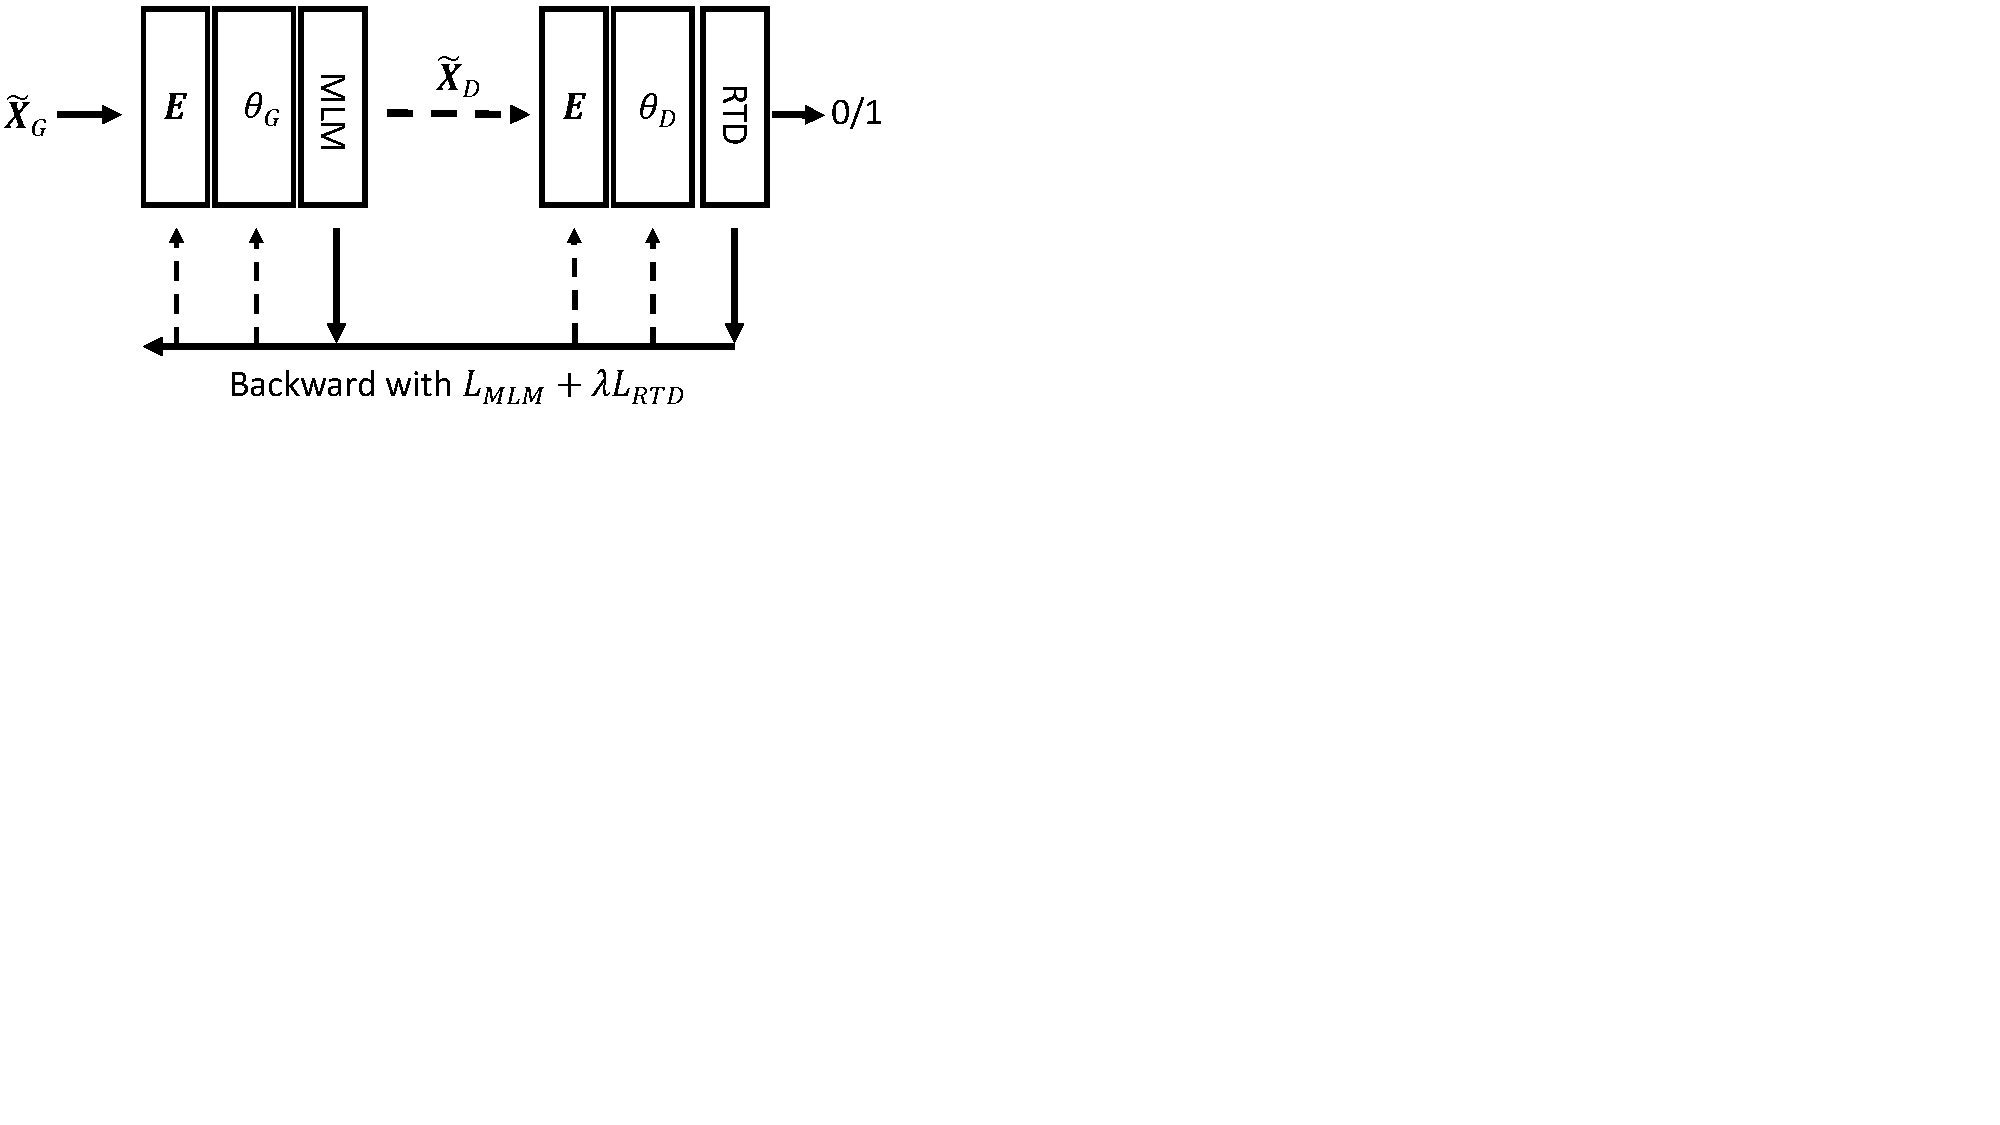
\includegraphics[width=0.31\linewidth,trim={0.1cm 11.8cm 18.5cm 0.1cm},clip]{figures/LRTD-a.pdf}
}
\hfill
\subfloat[无嵌入共享]{
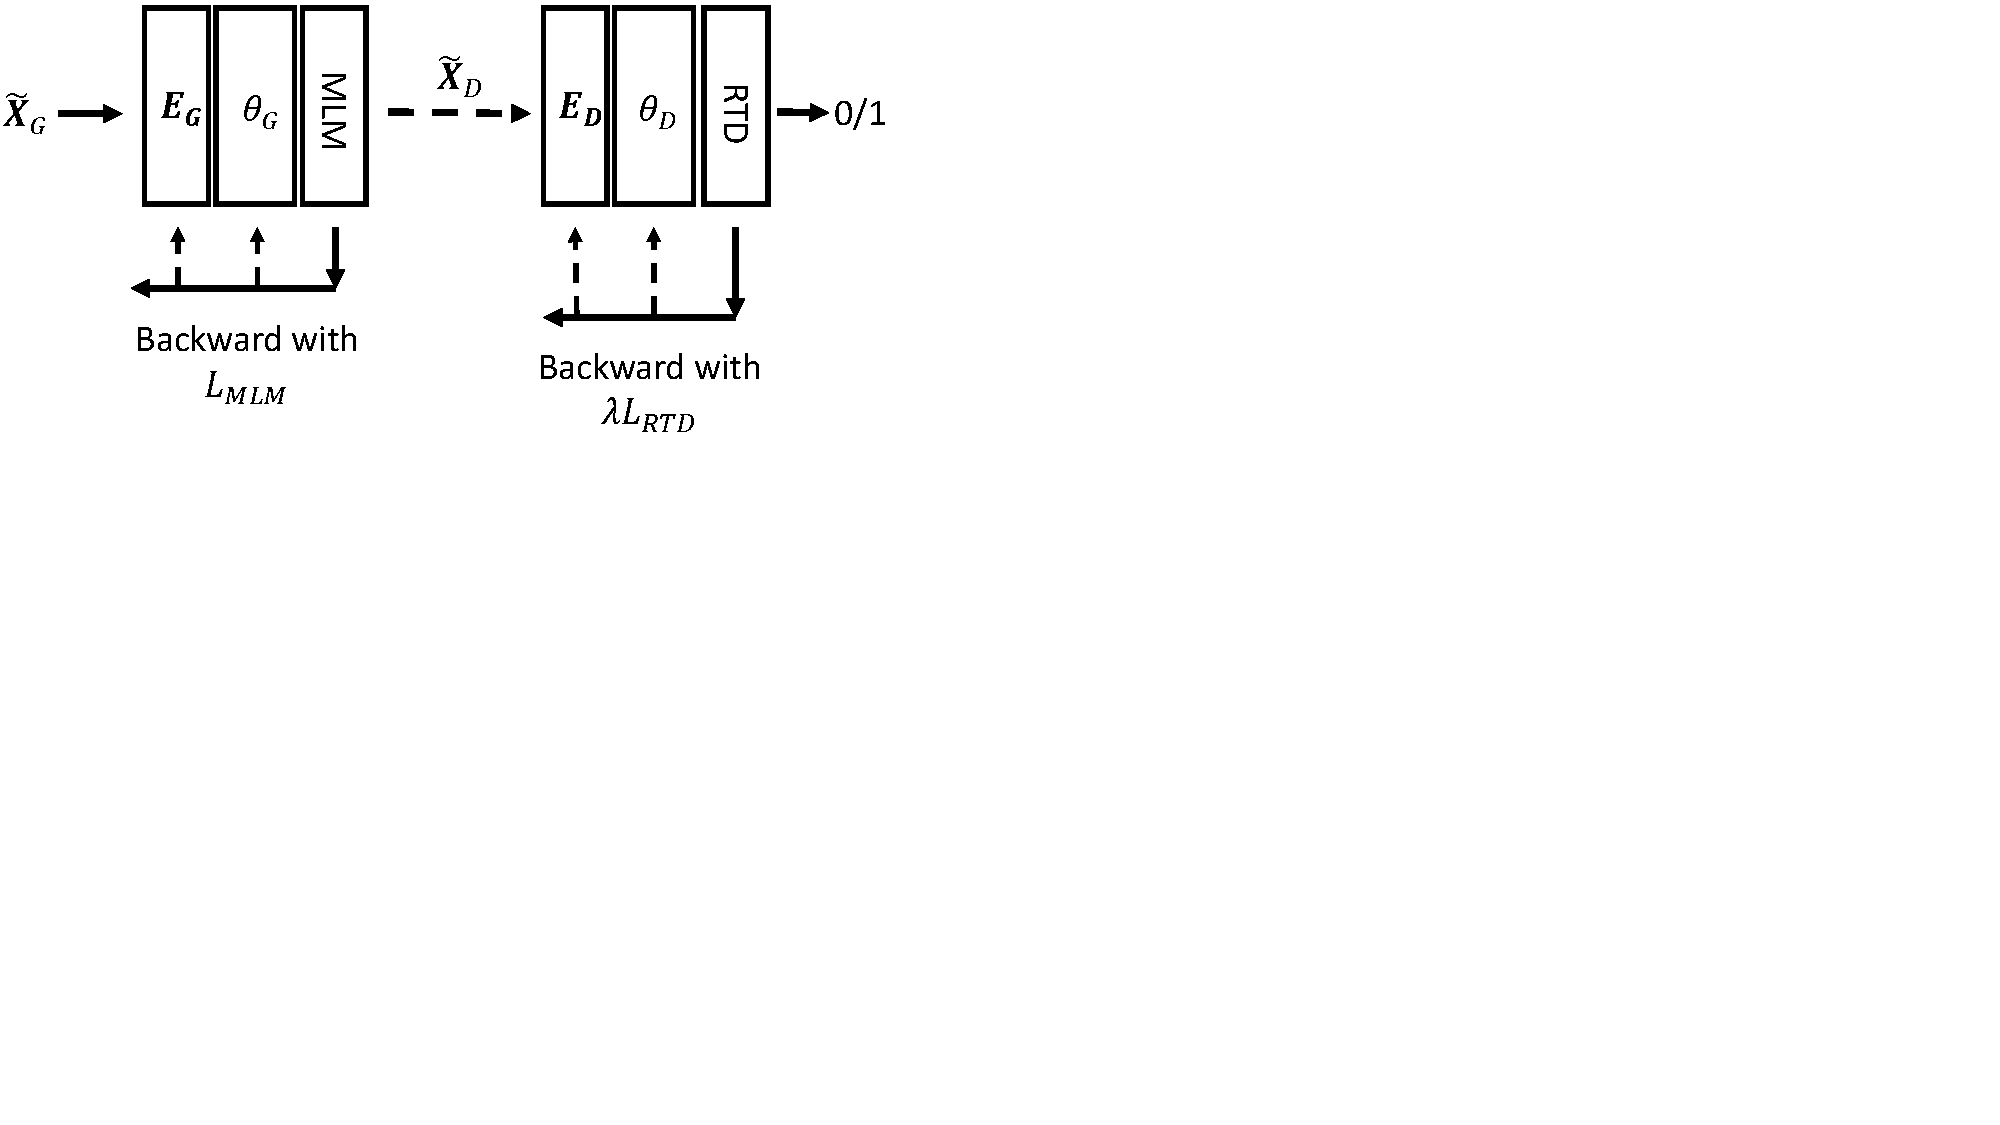
\includegraphics[width=0.31\linewidth,trim={0.1cm 11.7cm 18.5cm 0.1cm},clip]{figures/LRTD-b.pdf}
}
\hfill
\subfloat[梯度解耦嵌入共享]{
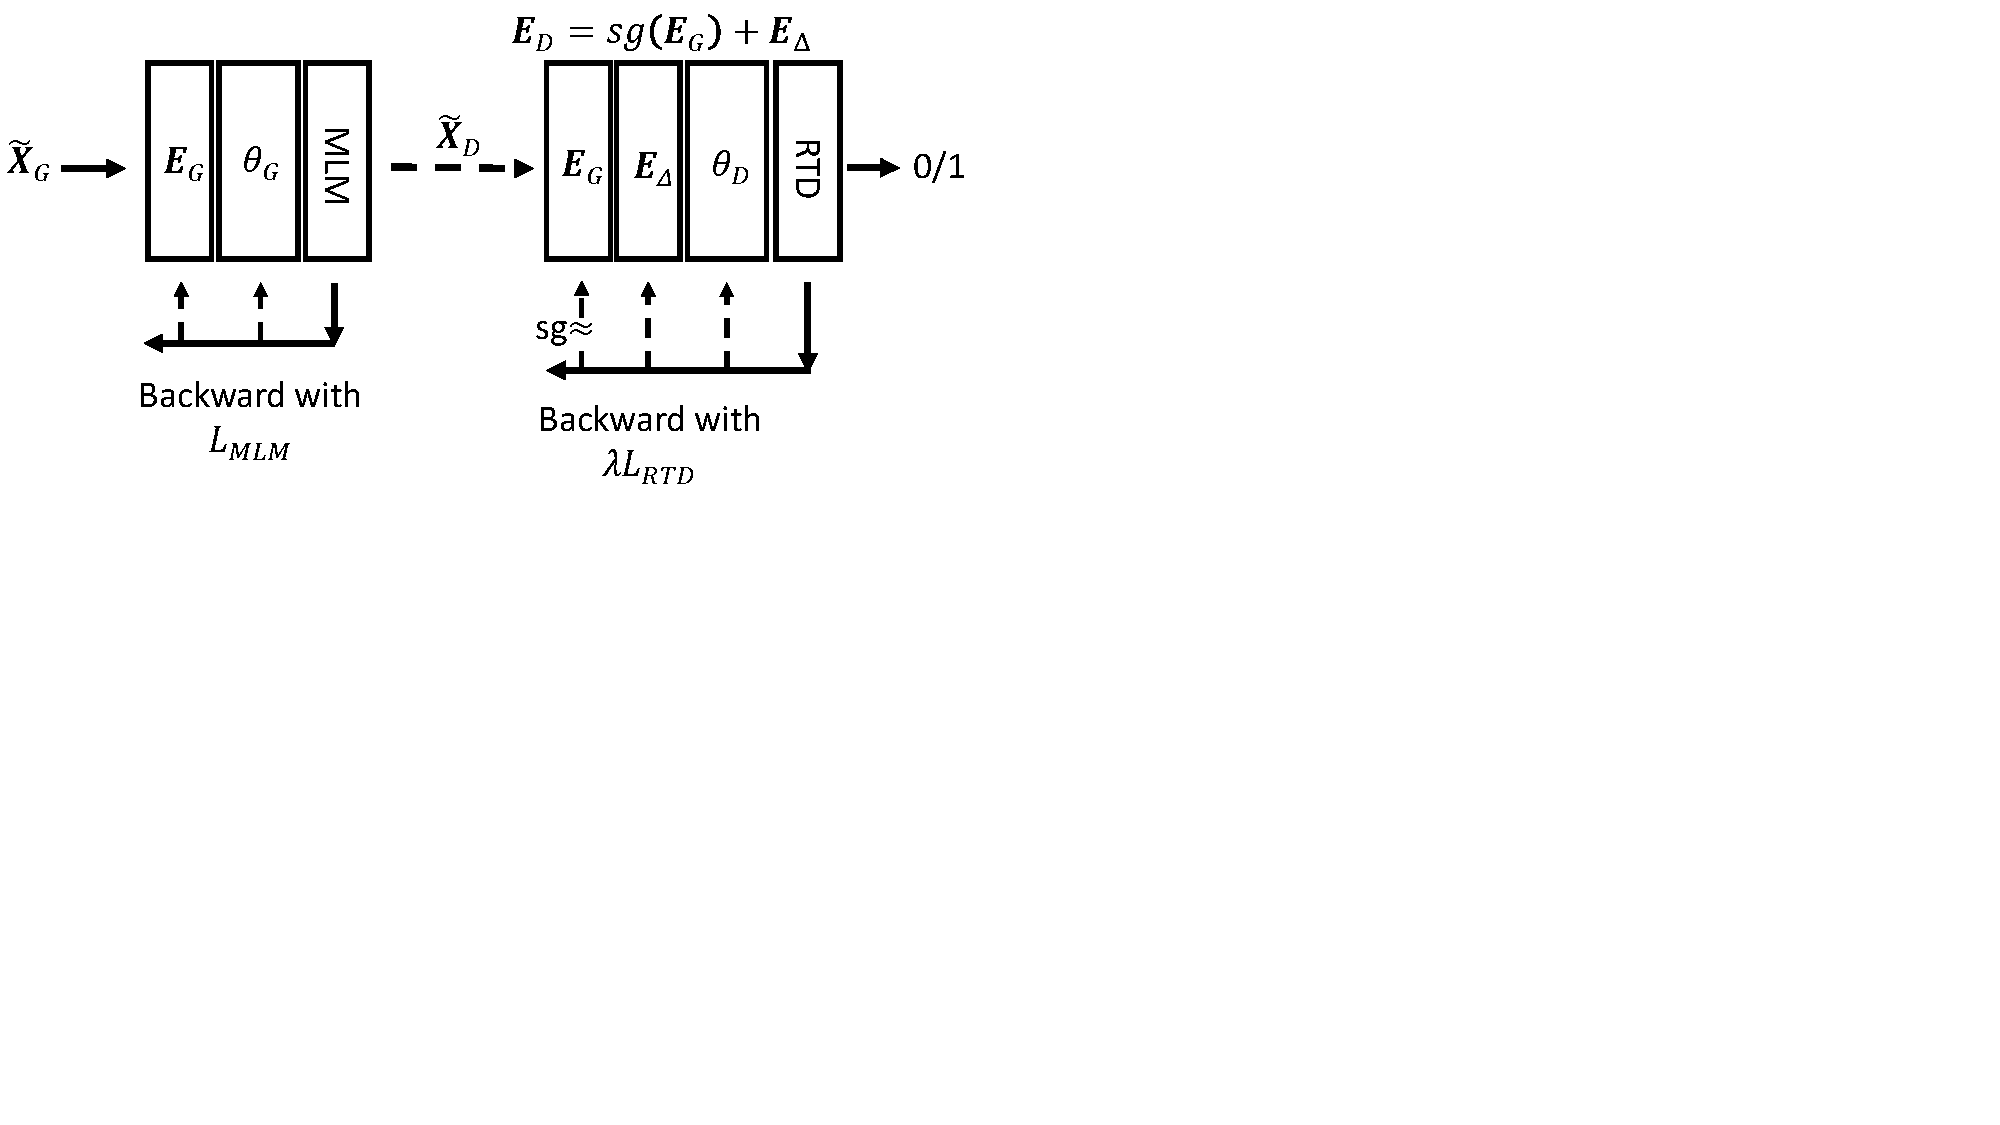
\includegraphics[width=0.31\linewidth,trim={0.1cm 10.4cm 17.5cm 0.1cm},clip]{figures/LRTD-c.pdf}
}
\caption{不同嵌入共享方法示意图 \cite{he2023debertav3improvingdebertausing}}
\label{fig:es}
\end{figure*}

DeBERTa V3 引入了一种名为梯度解耦嵌入共享(Gradient-Disentangled Embedding Sharing, GDES)的方法,旨在克服传统嵌入共享(Embedding Sharing, ES)和无嵌入共享(No Embedding Sharing, NES)所存在的不足,同时保留其优点。图 \ref{fig:es} 展示了不同嵌入共享策略的示意图。在嵌入共享(ES)策略中,参数 \(\mathbf{E}\)、\(\theta_G\) 和 \(\theta_D\) 在一次反向传播中依据损失函数 \(L_{\text{MLM}} + \lambda L_{\text{RTD}}\) 共同更新。而在无嵌入共享(NES)策略中,参数 \(\mathbf{E}_G\) 和 \(\theta_G\) 首先基于 \(L_{\text{MLM}}\) 进行反向传播更新,然后 \(\mathbf{E}_D\) 和 \(\theta_D\) 则依据 \(\lambda L_{\text{RTD}}\) 进行独立更新。与此不同,梯度解耦嵌入共享(GDES)方法首先根据 \(L_{\text{MLM}}\) 更新 \(\mathbf{E}_G\) 和 \(\theta_G\),接着则通过 \(\lambda L_{\text{RTD}}\) 和 \(\mathbf{E}_G\) 更新 \(\mathbf{E}_{\Delta}\) 和 \(\theta_D\)。在此过程中,停止梯度操作符 \(sg\) 被应用,以防止判别器对 \(\mathbf{E}_G\) 的更新。

如图 \ref{fig:es}(c)所示,梯度解耦嵌入共享方法允许生成器与判别器之间共享词嵌入,这使得两者能够从同一词汇表中学习并利用嵌入中蕴含的丰富语义信息。然而,与传统的嵌入共享方法相比,梯度解耦嵌入共享方法确保替换词元检测损失不会对生成器的梯度产生影响,从而避免了目标冲突带来的干扰和效率低下的问题。相反,该方法仅利用掩码语言模型损失来更新生成器的嵌入,确保生成器输出的一致性与连贯性。最终,梯度解耦嵌入共享方法能够实现与无嵌入共享相当的收敛速度,同时不牺牲嵌入的质量。

为实现梯度解耦嵌入共享,DeBERTa V3 将判别器的嵌入重新参数化为 \(\mathbf{E}_D = sg(\mathbf{E}_G) + \mathbf{E}_{\Delta}\),其中停止梯度算子 \(sg\) 防止梯度流经生成器的嵌入 \(\mathbf{E}_G\),仅更新残差嵌入 \(\mathbf{E}_{\Delta}\)。在训练过程中,\(\mathbf{E}_{\Delta}\) 被初始化为零矩阵,并依据无嵌入共享的训练流程进行模型训练。在每次迭代中,生成器首先为判别器生成输入,并利用掩码语言模型损失更新 \(\mathbf{E}_G\) 和 \(\mathbf{E}_D\)。随后,判别器在生成的输入上进行操作,并通过梯度解耦嵌入共享损失仅更新 \(\mathbf{E}_D\) 的参数 \(\mathbf{E}_{\Delta}\)。训练完成后,\(\mathbf{E}_{\Delta}\) 将被加到 \(\mathbf{E}_G\) 上,得到的矩阵作为判别器的最终嵌入 \(\mathbf{E}_D\)。

DeBERTa V3 进行了广泛的实验,以评估梯度解耦嵌入共享方法相较于嵌入共享和无嵌入共享的有效性。实验结果表明,梯度解耦嵌入共享是一种有效的权重共享策略,适用于结合掩码语言模型和替换词元检测的预训练语言模型。因此,DeBERTa V3 模型在 Kaggle 排行榜和深度学习领域展现出卓越的性能。在本实验中,使用的 DeBERTa 系列模型包括 DeBERTa-V3-Base 和 DeBERTa-V3-Large,其模型参数如表 \ref{tab:deberta-parameter} 所示。

\begin{table*}[htbp]
\centering
\caption{DeBERTa-V3-Base 和 DeBERTa-V3-Large 模型参数} \label{tab:deberta-parameter}
\begin{tabular}{lcc}
\toprule
               & \multicolumn{1}{l}{\textbf{DeBERTa-V3-Base} \cite{he2023debertav3improvingdebertausing}} & \multicolumn{1}{l}{\textbf{DeBERTa-V3-Large} \cite{he2023debertav3improvingdebertausing}} \\ \midrule
Transformer 层数 & 12                                           & 24                                            \\
隐藏层维度          & 768                                          & 1024                                          \\
词汇表大小          & 128K                                         & 128K                                          \\
主干网络参数量        & 86M                                          & 304M                                          \\
嵌入层参数量         & 98M                                          & 131M                                \\ \bottomrule         
\end{tabular}
\end{table*}

\section{大语言模型技术}
\label{sec:rw-llm}

\subsection{ChatGPT}
\label{sec:TOSWT-gen-chatgpt}

最早推出的 ChatGPT \cite{chatgpt},也被称为 GPT-3.5(Generative Pre-trained Transformer 3.5),是 OpenAI 在 GPT-3 的基础上进行优化而构建的大型语言模型(LLM)。该模型属于生成式预训练模型家族,基于 Transformer 架构,展现出在自然语言生成(NLG)、理解(NLU)以及多任务处理等方面的卓越性能,广泛应用于学术写作、代码生成和智能客服等多个领域。

ChatGPT 基于 Transformer 架构的神经网络设计,其核心特征在于自注意力机制(Self-Attention)的应用。这一机制能够有效捕捉文本序列中的长距离依赖关系,并支持并行计算,从而提高训练效率。研究表明,该模型的某些版本参数规模可达 1750 亿,通过构建深层网络结构并结合海量训练数据(包括互联网公开文本和学术文献等),显著提升了模型的性能表现。在训练方法上,ChatGPT 采用了“预训练与微调”的混合范式:首先通过无监督学习从大规模语料库中提取通用语言表征,随后结合有监督微调技术进行任务适配。此外,该模型创新性地引入了人类反馈强化学习 \cite{kaufmann2024surveyreinforcementlearninghuman}(Reinforcement Learning from Human Feedback, RLHF)方法,从而有效优化模型输出与人类价值观之间的对齐性。

ChatGPT(GPT-3.5)作为 OpenAI 首个面向公众的大规模对话式人工智能,具有里程碑式的技术发展意义。其历史贡献主要体现在三个方面:首先,它通过免费交互的形式使得具有 1750 亿参数的大型模型能力得以普及,用户在短短两个月内突破一亿,成为历史上增长最快的消费级应用;其次,借助于指令微调和人类反馈强化学习(RLHF)的技术创新,显著增强了模型对人类意图的对齐能力,为后续对话模型的训练框架奠定了基础;最后,其在代码生成、教育辅助等领域的跨领域应用展示了通用人工智能的潜力,例如成功通过美国律师考试并催生了 AIGC 产业生态。然而,随着后续模型(如 GPT-4 和 GPT-4o)的推出,其局限性逐渐显现:上下文窗口仅为 3000 词(而 GPT-4 可达 2.5 万词),在复杂推理和数学计算方面的准确率低于 GPT-4(例如在 LSAT 考试中,GPT-4 的得分高出 15\%);此外,其仅支持文本交互,缺乏多模态能力;知识的时效性受限于 2021 年的训练数据,且幻觉控制能力较弱,事实错误率比 GPT-4 高出约 40\%。这些不足促使模型向更大参数规模、更优对齐性及更低推理成本的方向不断演进。

从技术迭代的角度来看,GPT-3.5 的突破性在于首次验证了大规模预训练模型与人类反馈相结合的优化方案的可行性。然而,其单模态架构及有限的推理能力在专业领域的应用中逐渐显得不足。例如,OpenAI 推出的新一代模型 GPT-4 通过引入多模态处理和万亿级参数,在医学诊断、法律分析等任务中展现出更高的可靠性。而 GPT-4o 则进一步整合了音频和视频交互能力,实现了更为自然的人机交互体验。

\subsection{GPT4o}
\label{sec:TOSWT-gen-gpt4o}

GPT-4o \cite{gpt4o} 是 OpenAI 于 2024 年 5 月推出的下一代多模态大语言模型,其中的 "o" 代表 "omni"(全能),标志着其在文本、音频和视觉模态的端到端处理能力上取得了显著突破。该模型采用统一的 Transformer 架构,能够通过单一神经网络直接处理多模态输入(包括文本、图像和音频的任意组合),并生成文本、音频和图像输出的任意组合,从而消除了传统多模态系统中不同模型间转换所带来的延迟问题。GPT-4o 实现了跨文本、视觉和音频的端到端训练,意味着所有输入和输出均由同一神经网络处理。在技术层面,该模型通过改进的词元化(tokenization)方法,将音频特征和视频帧序列编码为与文本相同的表示形式,并利用多头注意力机制实现跨模态的语义关联,能够在低至 232 毫秒的时间内响应音频输入,平均响应时间为 320 毫秒,这与人类在对话中的反应时间相当。

与前代模型相比,GPT-4o 展现出三方面显著优势:首先,其多模态能力实现了质的飞跃,能够执行如图像内容分析生成食谱以及通过呼吸声识别情绪状态等复杂任务;其次,其非英语语言处理能力显著提升,支持 50 种语言的实时翻译,尤其在非拉丁语系文字(如韩语和阿拉伯语)的识别准确率提高超过 20\%;最后,其运行效率得到了显著优化,API 成本较 GPT-4 Turbo 降低了 50\%,推理速度提升了两倍。

\subsection{Gemini}
\label{sec:TOSWT-gen-gemini}

Gemini \cite{geminiteam2024geminifamilyhighlycapable} 是 Google DeepMind 开发的一系列多模态大语言模型,标志着谷歌在通用人工智能领域的重要进展。该系列模型于 2023 年 12 月正式推出,其核心创新在于采用原生多模态架构,能够同时处理文本、图像、音频、视频及代码五种信息类型。与传统多模态模型不同,Gemini 从预训练阶段起便利用统一的神经网络处理多模态输入,通过改进的词元化(tokenization)方法将不同模态的数据编码为统一表示,并通过多头注意力机制实现跨模态的语义关联。这一设计使其在复杂推理任务中表现卓越,例如能够理解手写的物理题解答并指出错误推理步骤,或将视觉信息转化为编程代码。在技术层面,Gemini 采用 TPUv4/v5e 加速器进行训练,其训练数据涵盖网络文档、学术文献和多语言语料,并通过人类反馈强化学习 \cite{kaufmann2024surveyreinforcementlearninghuman} (RLHF)优化输出的一致性。

尽管 Gemini 在多模态理解和复杂推理方面展现出优势,但仍存在一定的局限性。早期版本受到质疑,认为其测试分数夸大且演示视频存在剪辑问题,此外在非英语任务中的性能相对较弱。与后续模型相比,Gemini 缺乏动态更新机制,其在专业领域(如医学和法律)的微调效果有待提升。这些不足促使谷歌朝着更大参数规模、更低推理成本和更专业化的方向迭代,例如发布了开源模型 Gemma(20 亿/70 亿参数)。总体而言,Gemini 系列通过原生多模态架构和规模化训练基础设施,为通用人工智能的发展提供了重要的技术范式。

\subsection{Qwen}
\label{sec:TOSWT-gen-qwen}

通义千问 \cite{qwen2025qwen25technicalreport}(Qwen)是阿里云自主研发的一系列超大规模语言模型,作为中国人工智能领域的重要代表,其技术进步和产业应用充分体现了国产大模型的发展历程。该模型系列于 2023 年 4 月 11 日正式发布,其名称蕴含双重含义:“通义”象征着模型在跨领域知识理解方面的广泛适用性,而“千问”则源自中国古代百科全书《千问》,彰显其处理复杂问题的能力。在技术架构方面,通义千问采用了改进的 Transformer 结构,通过旋转位置编码 \cite{su2023roformerenhancedtransformerrotary}(RoPE)增强了对长序列的建模能力。此外,该模型创新性地结合了非绑定式嵌入(un-tied embeddings)与 RMSNorm 层进行优化,使其在 72B 参数版本中实现了 2048 个词元的上下文窗口支持。值得一提的是,其开源模型 Qwen1.5-110B 采用了稀疏专家混合(MoE)架构,并在 2024 年 5 月发布的 2.5 版本中,逻辑推理和代码能力较前一代提升了 16\% 和 10\%。

该模型的核心竞争力体现在三个主要方面:多模态融合、产业适配性以及开源生态系统的构建。在模态支持方面,通义千问2.0 已实现对文本、图像和音频的端到端处理,其多模态理解能力使其能够执行从商品设计草图生成营销文案等复杂任务。在产业应用方面,阿里云通过实施“云智一体”战略,将模型能力深度嵌入电商、医疗和金融等多个场景。例如,通义灵码智能编程助手能够完成 85\% 的常规代码生成任务,从而显著提升开发效率。在开源策略方面,截至 2025 年,通义千问已发布从 1.8B 到 110B 参数的七款开源模型,累计下载量超过 700 万次。其中,Qwen-72B 在 MMLU 基准测试中达到了与 Llama3-70B 相当的精度。

与同期国际模型相比,通义千问展现出显著的差异化特征。其训练数据中包含超过 30\% 的高质量中文语料,使其在古文解析和中文创意写作等任务上表现优于同等规模的 GPT-3.5 模型。在商业应用方面,通过实施 API 价格策略(2 元/1M tokens)及轻量化部署方案(例如与联发科天玑9300芯片的适配),显著降低了企业的使用门槛。然而,该模型在处理非拉丁语系的多语言任务时,其准确率仍比 GPT-4 低约 15\%。这些技术优势使通义千问成为中国大模型技术自主创新与全球竞争的重要案例,其发展路径为学术界在 AI 技术产业化方面的研究提供了典型的参考样本。

\subsection{DeepSeek}
\label{sec:TOSWT-gen-ds}

DeepSeek V3 \cite{deepseekai2024deepseekv3technicalreport} 是中国深度求索公司(DeepSeek)于2024年12月发布的新一代多模态大语言模型,标志着国产大模型在技术创新与成本控制方面的重要里程碑。该模型采用混合专家(MoE)架构,总参数量达到6710亿,其中每个词元激活370亿参数,通过动态路由机制实现计算资源的高效分配。在技术层面,DeepSeek V3 创新性地结合了多头潜在注意力机制(MLA)与 FP8 混合精度训练。前者通过低秩压缩键值对有效降低内存占用,后者则在矩阵乘法等计算密集型操作中采用 FP8 格式,使得训练成本控制在557.6万美元,仅为 GPT-4o 等主流模型的十分之一。在14.8万亿 token 的预训练基础上,模型通过监督微调和强化学习进一步优化性能,其生成速度达到60 TPS(每秒事务处理量),较前代 V2.5 提升了三倍,显著改善了交互的流畅性。

在性能表现方面,DeepSeek V3 展现出在多个领域的竞争优势。在知识类任务(如 MMLU 和 GPQA)中,其表现接近于 Claude-3.5-Sonnet,而在数学竞赛(如 AIME 2024 和 CNMO 2024)中,其成绩超越了所有开源和闭源模型。此外,其代码生成能力可与 85\% 的人类编程选手相媲美。特别是在中文处理方面,凭借 30\% 的高质量中文语料进行训练,该模型在古文解析和创意写作等任务中优于同等规模的国际模型。2025年3月发布的 V3-0324 版本进一步增强了前端开发能力,能够根据单一提示自动生成包含交互控件和赛博朋克风格界面的完整网站,开发者将其誉为“编码领域的标杆”。该模型支持 128K 的上下文窗口(开源版),在长文本理解任务(如 DROP 和 LongBench v2)中的平均表现领先于行业标准。

DeepSeek V3 的商业化与开源策略是其另一显著特色。其 API 定价极具竞争力,输入和输出词元的成本分别为每百万词元 0.27 美元和 1.10 美元,较国际同类产品降低超过 50\%。该模型采用 MIT 开源协议,允许商业用途及二次开发,截至 2025 年,已实现 700 万次下载,促进了 AI 技术在边缘设备上的部署。其应用场景涵盖智能编程(如通义灵码助手)、金融风险控制及教育辅导等多个领域。在电商平台的数据分析场景中,该模型能够实时识别欺诈交易并生成可视化报告。

尽管 DeepSeek V3 的表现十分出色,但其仍存在一定局限性,尤其是在处理复杂音频和视觉输入时,其幻觉率比文本模态高出约 20\%。然而,DeepSeek V3 现有的诸多优势特性使其成为研究 AI 技术普惠化与计算效率优化的典型案例,为中国大模型在全球竞争中的发展提供了重要参考。

\section{AI 生成文本检测技术}
\label{sec:llmdetect}

大型语言模型(LLMs)的迅速发展促使对检测 AI 生成文本的方法进行深入研究。在 ChatGPT 发布之前,GLTR \cite{gehrmann_gltr_2019} 作为一种文本检测工具,通过一系列统计分析技术识别由不同采样策略生成的文本特征。GLTR 有效地将人类对生成文本的检测准确率从 54\% 提升至 72\%,彰显了其在帮助非专业人士区分人类与机器生成内容方面的实用性。

另一个重要的贡献是人类 ChatGPT 比较语料库 \cite{guo_how_2023}(HC3),该语料库是在 ChatGPT 发布后开发的。HC3 数据集包含来自人类专家与 ChatGPT 的数万个响应,涵盖金融、医学和法律等多个领域。这一数据集使得对 ChatGPT 的响应与人类输出进行全面评估成为可能,从而揭示了 LLMs 的能力与局限性。此外,HC3 还促进了检测系统的发展,旨在识别文本是由 ChatGPT 还是人类生成的。

LLM-Detector \cite{wang_llm-detector_2024} 针对现有人工智能生成文本检测模型所面临的挑战进行了研究,这些模型通常因领域内过拟合而在领域外表现不佳。该研究通过收集人类专家和多种大语言模型的回复,基于大型语言模型提出了一种新颖的检测方法,利用指令调优来增强文档级和句子级的检测能力。实验结果表明,该方法在性能上显著优于基线方案,展现出强大的泛化能力。

SeqXGPT \cite{wang_seqxgpt_2023} 通过构建一个包含大语言模型生成句子与人类写作内容的数据集,引入了句子级检测挑战。该方法利用来自白盒 LLMs 的对数概率列表,结合卷积网络和自注意力机制以提高检测准确性。结果显示,SeqXGPT 在句子和文档级检测任务中均优于现有方法,进一步强调了有效检测机制的必要性。

针对人工智能生成文本来源追踪的问题 \cite{li_origin_2023},已有研究提出了一种创新的算法,旨在检测和追踪人工智能生成的内容。该方法通过对比特征有效区分由不同模型生成的文本,能够在白盒和黑盒环境中均发挥作用。研究结果突显了人工智能部署所带来的伦理影响,以及追踪生成文本来源机制的重要性,为关于人工智能系统问责制的持续讨论提供了重要的理论支持。

然而,现有的方法 \cite{gehrmann_gltr_2019, guo_how_2023, wang_llm-detector_2024, wang_seqxgpt_2023} 尚未满足我们对文本来源于特定大型语言模型的检测需求。大多数研究在分类任务上表现较为粗糙,仅能识别文本是由人类还是机器生成,无法进一步确定文本的具体来源。尽管少部分研究 \cite{li_origin_2023} 实现了识别文本来源于特定大型语言模型的目标,但其实现方式依赖于白盒测试,必须获取与待检测模型一致或相似的模型生成的特征向量才能进行判断。在当前大多数大型语言模型均为闭源的环境下,这种方法几乎缺乏扩展性和可操作性。

\section{本章小结}
\label{sec:rw-conclusion}

本章回顾了当前自然语言处理领域的相关工作,重点聚焦于文本生成技术和预训练语言模型的进展。首先,我们深入分析了Transformer架构的优势,强调了其在大语言模型中的广泛应用。自2017年提出以来,Transformer因其卓越的并行处理能力和长距离依赖建模能力,迅速成为自然语言处理研究的核心。通过自注意力机制,Transformer能够有效捕捉输入序列中各个部分之间的关系,从而显著提高了模型在处理大规模文本数据时的训练效率和表达能力。

随后,我们详细讨论了BERT模型的结构及其在预训练和微调过程中的创新。BERT不仅在机器阅读理解等多个任务中取得了显著的性能提升,还引入了预训练-微调的二阶段训练范式,使得模型能够在预训练阶段学习通用的语言表示,而在特定任务中进行微调。这一策略极大地提升了模型的适应性和性能,标志着自然语言处理领域的一次重大变革。在预训练语言模型的讨论中,我们提及了如GPT、RoBERTa和DeBERTa等模型的相继出现,这些模型在BERT的基础上进行了不同程度的改进,进一步推动了预训练模型的研究和应用。

此外,我们介绍了多种大型语言模型,包括 ChatGPT、GPT4o、Gemini、Qwen 和 DeepSeek。研究表明,大语言模型正沿着多模态融合、计算效率优化和专业化应用三个维度持续演进:从ChatGPT的单模态文本处理到GPT-4o的端到端多模态交互,体现了模态整合能力的突破;Gemini的原生多模态架构与DeepSeek V3的混合专家设计展示了计算效率的优化路径;而通义千问的产业适配策略则凸显了专业化应用的重要性。这些模型在提升语言理解、跨模态推理等核心能力的同时,仍面临幻觉控制、多语言处理等方面的技术挑战,其发展轨迹为后续研究提供了重要的技术参照和产业化启示。这五个大语言模型这些模型将在后面的章节中用于构建改写文本数据集。

最后,本章探讨了AI生成文本的检测技术,介绍了多种现有方法及其在实际应用中的效果与局限性。尽管GLTR、HC3、LLM-Detector、SeqXGPT等工具在识别生成文本方面取得了一定的成效,但仍面临特定大型语言模型检测的挑战。尤其是在当前许多大型语言模型为闭源的环境下,现有方法在文本来源追踪和特定模型检测方面的适用性显得尤为重要。

综上所述,本章的讨论为理解当前技术状态及未来研究方向提供了重要视角,为本论文的研究奠定了坚实的基础。通过对Transformer架构、BERT模型及AI文本检测技术的全面回顾,我们为后续的研究和实验提供了必要的理论支持和实践指导。
%%==================================================
%% chapter01.tex for BIT Master Thesis
%% modified by pinren lu
%% version: 0.1
%% last update: Dec 25th, 2016
%%==================================================
% TOSWT 数据集构建

% 1. 引言
% 2. 方法
%    1. ChatGPT3.5
%    2. GPT4o
%    3. Qwen
%    4. DS
%    5. Gemini
% 3. 数据集介绍
% 4. 本章小结

\chapter{模型改写文本检测数据集构建方法}
\label{chap:TOSWT}

\section{引言}
\label{sec:TOSWT-intro}

在前两章中, 我们详细介绍了探测 AI 生成文本的前世今生。在本章节中,我们将构造出属于自己的数据集。我们的数据集名称叫做追踪学生写作文本来源数据集(Tracing the Origins of Students’ Writing Texts, 以下简称 TOSWT 数据集)在前人的基础上,我们首先要在教育学领域,为教师提供分析文本来源的工具数据集,其次要将数据集更加细粒度,例如探索句子级别,使得实验有着更广泛的应用性,可以帮助教师敏锐地指出学生文本中哪一句经过了什么大型语言模型的修改。

在 Learning Agency Lab 发布的 Automated Essay Scoring 2.0 \cite{learning-agency-lab-automated-essay-scoring-2} (AES2) 数据集的基础上,TOSWT 数据集应运而生。AES2 数据集是一个用于自动写作评价的数据集,包含了 10,584 篇由 9-12 年级学生撰写的短文,并为每篇文章提供了 1-6 分的评分,其中高质量的文本将获得更高的评分。我们在 AES2 数据集的基础上,对原始数据进行了清洗,利用正则表达式替换非 ASCII 字符,并使用句子分割工具将短文划分为句子。此后,我们选用了一种 prompt 进行引导大语言模型改写处理后的短文。

Automated Essay Scoring 2.0 数据集发布于 Kaggle 平台上,为解决自动写作评估问题召开比赛,作为比赛用数据集。短文写作是评估学生学习和表现的重要方法。教育者手工评分也很耗时。自动写作评估(Automated Writing Evaluation, AWE)系统可以对论文进行评分,以补充教育者的其他努力。自动写作评估系统还允许学生定期及时地收到关于他们写作的反馈。但是,由于其成本,该领域的许多进步并没有广泛地提供给学生和教育者。评估学生写作的开源解决方案需要用这些重要的教育工具到达每个社区。

以前开发开源自动写作评估系统的努力受到小型数据集的限制,这些数据集不是广泛性的,也不专注于常见的短文格式。之前在 Kaggle 平台上举办的第一届自动论文评分竞赛对学生写的简短答案进行评分,然而,这是一项课堂上不常使用的写作任务。为了改进以前的努力,需要一个更广泛的数据集,包括高质量、现实的课堂写作样本。此外,为了扩大影响,数据集应该包括跨经济和地点人群的样本,以减轻算法偏见的可能性。

因此 Learning Agency Lab 发布 Automated Essay Scoring 2.0 数据集,这是当时最大的开放获取写作数据集,且该数据集符合当时学生的评估标准。AES2 数据集示例如表 \ref{tab:AES2-example} 所示,其中仅列举 1-3 分数据样例各一个,并省略掉了原文中的换行符“\textbackslash{}n”。

\begin{table*}[htbp]
\caption{AES2 数据集数据示例} \label{tab:AES2-example}
\begin{tabular}{cp{13.3cm}c}
\toprule
\textbf{essay\_id} & \multicolumn{1}{c}{\textbf{原文}}  & \textbf{评分} \\ \midrule
eb8f967 & Honestly, who would think there   is "Alien Form" on Mars, I mean some of the people are just plain   stupid, and some have facts and details. I think that these so called aliens   are just Fallen Angels, because I read the Bible. These are simply just   natural lanforms. When you take a look at this structure it does look like   a humans face. Then again, I dont think it is an alien monument because, from   how far you look at it and how far they took pictures from it. I don't think   aliens could have made a face a couple miles long, it would have to take   years to do this. Anyhow, I do believe there was life on the planet, I know   there was water, because they have lots of craters, canyons, and   mountains. My conclusion is, they were formed by natural occurances. As in   the passage they compared the face to some features in the American West such   as, Middle Butte, and Snake River Plain of Idaho in the West. These   conlusions matched the face up to natural formation. The face formation is   known as a messa or a plataeu.  & 1  \\ \midrule
7913c3a & My position on driverless cars   is very nutral. Like the passage stated there are a lot pros and cons when it   comes to this topic, such as numerous types of road blocks like accidents and   construction. When it comes to the diverless car getting to an accident   people are confused on who it should be to blame the manufacturer, or the   passenger. I personaly believe the passenger should be to blame, it doesn't   matter how advanced the technology is something is bound to go wrong so you   should always be on alert. When it comes to some of the pros there are   some strong ones. Driving will be a lot safer once a majority of people own a   self driving car. There will be almost no accidents do to texting, falling   asleep at the wheel, and drunk driving. Once we get to the point of almost   everyone owning a self diving car they will most likely be eco-friendly. & 2  \\ \midrule
5d147d6 & Having the new technolgy would   help every teacher and school around the world. By being able to tell how a   student feels the teacher can change the way they would teach the classes or   the way they would a explain a lesson. The computer would tell the teacher   how the students are feeling. It would be valuable to have that type of   technolgy in class room becuase it would make teachers jobs less   complicated. Using the new technology would hellep teacher understand the   students in knowing how they feel whithout having to ask them. "A   classroom computer could recognize when a student is becoming confused or   bored". In this example Dr. Huang explains what the cumputer is able to   do it. By telling how a student is feeling this can help teachers be the   teacher not having to ask every student how they feel. The computer would do   it for the teacher. By having the computer know how the student feels the   teaacher can focus more on exlpaing the lesson better and making it easier to   understand for students to understand. "This could modify the   lesson,like an effective human instuctor" Dr. Huang elpaians that   the computer can change it is teaching the lesson like a teacher would it   also states that it would do it as effective as a human instructor would.   That means having that technolgy would help improve schools teach improve   classes and the way people are being tought. & 3  \\ \bottomrule
\end{tabular}
\end{table*}

在 AES2 数据集中,他们应用如下的评分标准来给学生写作短文打分,分数从低到高是 1 分(最低)到 6 分(最高)。与下面所描述的评分标准一样,每个分数之间的差距(例如 1-2 分、3-4 分、4-5 分)应尽可能相等。

\begin{itemize}
\item[\textbullet] 
\textbf{6 分}:该类文章展现出清晰且稳定的高水平能力,尽管可能存在一些小错误。典型的文章能就议题有效且深刻地阐述观点,展现出卓越的批判性思维;文章能从原文中选取恰当的例子、理由及其他证据来支撑其观点;文章结构合理、重点突出,展现出清晰的连贯性和流畅的思路推进;文章语言运用娴熟,词汇丰富、准确、恰当,句子结构富有变化;文章在语法、用法和书写规范方面基本没有错误。

\item[\textbullet] 
\textbf{5 分}:该类文章展现出较为稳定的高水平能力,尽管偶尔会出现错误或质量上的小瑕疵。典型的文章能就议题有效阐述观点,展现出较强的批判性思维;文章通常能选用恰当的例子、理由及其他证据来支撑其观点;文章结构良好、重点明确,展现出连贯性和思路推进;文章语言运用熟练,词汇恰当,句子结构有变化;文章在语法、用法和书写规范方面基本没有错误。

\item[\textbullet] 
\textbf{4 分}:该类文章展现出足够的能力,尽管在质量上会有起伏。典型的文章能就议题阐述观点,展现出合格的批判性思维;文章能运用足够的例子、理由及其他证据来支撑其观点;文章大致结构合理、重点突出,展现出一定的连贯性和思路推进;文章语言运用能力有所波动,词汇基本恰当,句子结构有一定变化;文章可能存在一些语法、用法和书写规范方面的错误。

\item[\textbullet] 
\textbf{3 分}:该类文章展现出正在发展的能力,但存在以下一项或多项不足:能就议题阐述观点,有一定批判性思维,但可能表现不稳定,或使用的例子、理由及其他证据不足以支撑观点;文章在结构或重点方面存在局限,或在连贯性和思路推进上有不足;文章语言运用有一定能力,但有时词汇使用较弱、选词不当,和 / 或句子结构缺乏变化或存在问题;文章可能存在语法、用法和书写规范方面的错误累积。

\item[\textbullet] 
\textbf{2 分}:该类文章展现出的能力较弱,存在以下一项或多项缺陷:对议题的观点模糊或极为有限,批判性思维薄弱;文章提供的例子、理由及其他证据不恰当或不充分,无法支撑观点;文章结构混乱和 / 或重点不明确,或在连贯性和思路推进上存在严重问题;文章语言运用能力极低,词汇量极为有限、选词错误,和 / 或句子结构频繁出现问题;文章存在严重的语法、用法和书写规范错误,在一定程度上影响了意思表达。

\item[\textbullet] 
\textbf{1 分}:该类文章展现出的能力极低或几乎没有,存在以下一项或多项严重缺陷:无法就议题提出可行的观点,或几乎没有提供证据支撑观点;文章毫无条理、没有重点,导致内容不连贯、逻辑混乱;文章在词汇使用上存在根本性错误,和 / 或句子结构存在严重缺陷;文章存在大量语法、用法或书写规范错误,严重干扰了意思的表达。
\end{itemize}

\section{问题阐述}
\label{sec:TOSWT-task}

文本来源追踪的任务可以数学化地表述为一个文本分类问题。我们定义一个文本语料库 \( T = \{t_1, t_2, \ldots, t_n\} \),其中每个文本 \( t_i \) 被表示为一个字符串,表示一段文本内容。我们的目标是将每个文本 \( t_i \) 分类到一个预定义的类别集合 \( C = \{c_1, c_2, \ldots, c_k\} \)。

这一过程可以通过以下步骤进行阐述:

1. \textbf{模型训练}:构建一个分类模型 \( f: T \to C \),该模型从训练数据集 $ D = \{(x_1, y_1),\\ (x_2, y_2), \ldots, (x_p, y_p)\} $ 中学习。在这里,\( y_i \in C \) 表示文本 \( t_i \) 的真实类别,而 \( x_i \in T \) 则代表相应的文本内容。模型通过学习这些样本之间的关系,逐渐形成对文本特征和类别之间映射的理解。

2. \textbf{分类过程}:对于新的文本 \( t_{new} \),特征提取过程生成 \( x_{new} \)。随后,利用训练好的模型进行预测:

   \[
   \hat{y} = f(x_{new})
   \]

   其中,\( \hat{y} \) 表示模型预测的类别。这个步骤的核心在于模型能够有效地将新文本映射到其可能的类别中,展现出其在特征空间中的判断能力。

3. \textbf{评估}:模型的性能通过计算一系列评估指标来进行评估,这些指标包括准确率、精确率、召回率和F1分数等。这些指标不仅帮助我们衡量模型在训练集上的表现,还能够评估其在未见数据上的泛化能力,从而确保模型在实际应用中的有效性。

通过上述步骤,我们能够系统地处理文本来源追踪的任务,将其转化为一个可操作的文本分类问题。这一方法论不仅为文本分类提供了清晰的框架,也为后续的研究和应用奠定了坚实的基础。


\section{模型改写文本检测数据集构建方法}
\label{sec:TOSWT-gen}

在 Learning Agency Lab 发布的 Automated Essay Scoring 2.0 (AES2) 数据集的基础上,TOSWT 数据集应运而生。AES2 数据集是一个用于自动写作评价的数据集,包含了 10,584 篇由 9-12 年级学生撰写的短文,并为每篇文章提供了 1-6 分的评分,其中高质量的文本将获得更高的评分。我们在 AES2 数据集的基础上,对原始数据进行了清洗,利用正则表达式替换非 ASCII 字符,并使用句子分割工具将短文划分为句子。此后,我们选用了一种 prompt 进行引导大语言模型改写处理后的短文。详细过程如图 \ref{fig:dataset-construct} 所示。

\begin{figure*}[htbp]
    \centering
    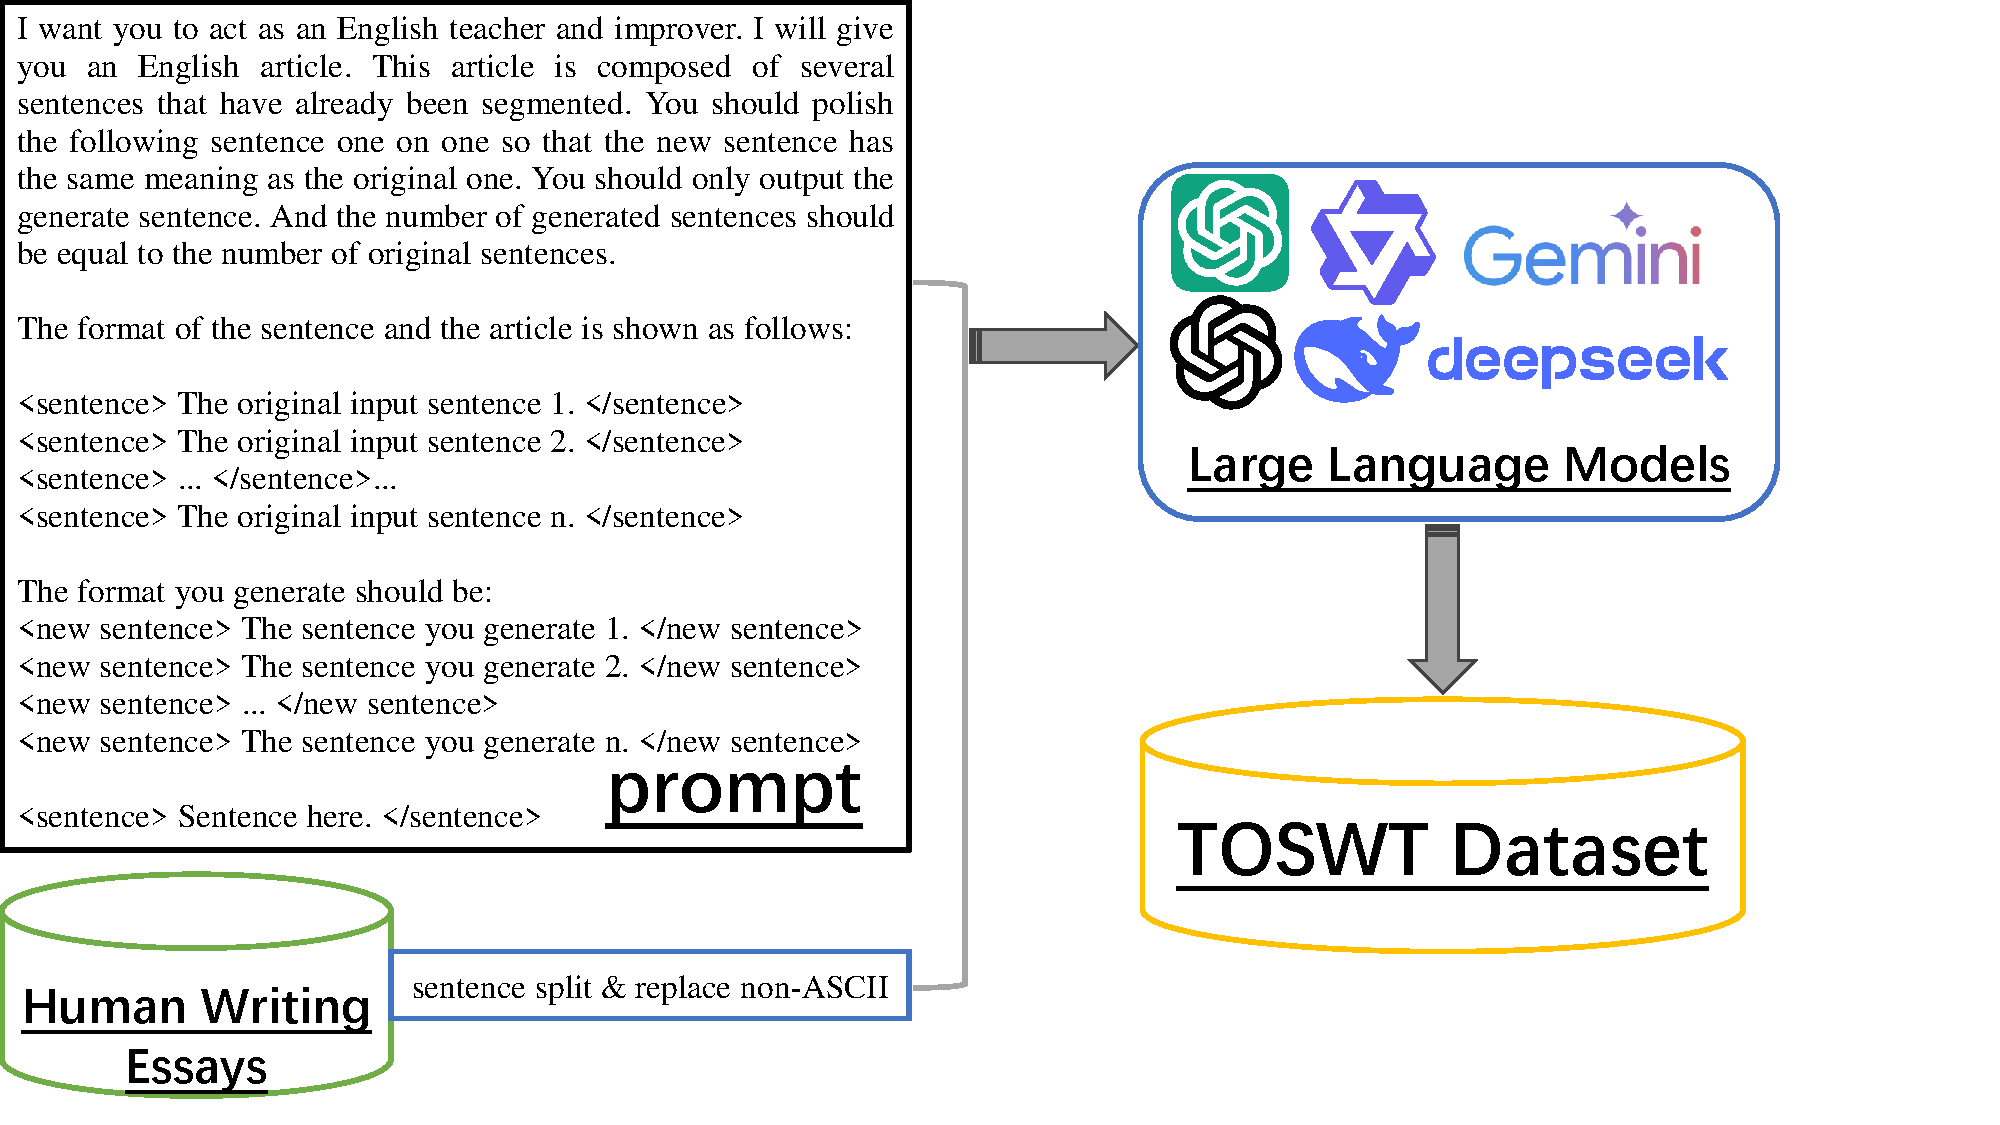
\includegraphics[trim=0 0 150 0, width=\textwidth]{figures/dataset-construct.pdf}
    % TOSWT 数据集构造流程。先将 AES2 中人类写作的短文经过句子分割、将非 ASCII 字符替换后,把每一句嵌入 prompt 中的 <sentence></sentence> 中。
    \caption{TOSWT 数据集的构造过程图}
    \label{fig:dataset-construct}
\end{figure*}

生成 TOSWT 数据集时使用 prompt 翻译表如表 \ref{tab:TOSWT-prompt} 所示。整体分成四个段落,第一段为任务的描述,二、三段则给出输入及输出的格式,最后第四段给予大语言模型输入的句子文本。

\begin{table*}[htbp]
    \centering
    \caption{Prompt 中英文对照表} \label{tab:TOSWT-prompt}
    \begin{tabular}{@{}p{7.5cm} p{7.5cm}@{}}
        \toprule
        \textbf{英文} & \textbf{中文} \\ \midrule
        I want you to act as a English teacher and improver. & 我希望你充当一名英语教师和改进者。 \\
        I will give you an English article. & 我将给你一篇英语文章。 \\
        This article is composed of several sentences that have already been segmented. & 这篇文章由几个已经被分割的句子组成。 \\
        You should polish the following sentence one on one so that the new sentence has the same meaning as the original one. & 你应该逐句润色以下句子,使新句子与原句具有相同的意思。 \\
        You should only output the generate sentence. & 你只需输出生成的句子。 \\
        And the number of generated sentences should be equal to the number of original sentences. & 生成的句子数量应与原句数量相等。 \\ \midrule
        The format of the sentence and the article is shown as follows: & 句子和文章的格式如下所示: \\
        <sentence> The original input sentence 1. </sentence> & <sentence> 原始输入句子 1。 </sentence> \\
        <sentence> The original input sentence 2. </sentence> & <sentence> 原始输入句子 2。 </sentence> \\
        <sentence> ... </sentence>... & <sentence> ... </sentence>... \\
        <sentence> The original input sentence n. </sentence> & <sentence> 原始输入句子 n。 </sentence> \\ \midrule
        The format you generate should be: & 你生成的格式应为: \\
        <new sentence> The sentence you generate 1. </new sentence> & <new sentence> 你生成的句子 1。 </new sentence> \\
        <new sentence> The sentence you generate 2. </new sentence> & <new sentence> 你生成的句子 2。 </new sentence> \\
        <new sentence> ... </new sentence> & <new sentence> ... </new sentence> \\
        <new sentence> The sentence you generate n. </new sentence> & <new sentence> 你生成的句子 n。 </new sentence> \\ \midrule
        <sentence> Sentence here. </sentence> & <sentence> 句子在这里。 </sentence> \\
        \bottomrule
    \end{tabular}
\end{table*}

这个 prompt 旨在帮助用户提升英语写作能力,具体通过将一篇英语文章进行润色与改进。它设定了用户作为英语教师和改进者的角色,引导用户逐句处理文本,以确保新生成的句子在意义上与原句一致。每个句子都被要求逐一润色,从而增强语言的流畅性和自然度。在执行过程中,用户将接收到一篇由多个已分割句子组成的文章。为了确保生成句子的数量与原句相等,prompt 设定了清晰的输出要求,用户只需专注于生成的新句子而无需担心格式问题。这种简洁的设计使用户能够更高效地进行文本修改。此外,prompt 提供了具体的格式示例,帮助用户理解所需的输出结构。这种结构化的指导不仅提高了工作效率,还确保了生成文本的规范性和一致性,进而为用户提供了系统的学习与实践体验。通过这种方式,用户能够在实际操作中获得更深刻的语言理解与应用能力。

\subsection{正则表达式替换非ASCII字符}
\label{sec:TOSWT-gen-reg}

正则表达式替换符号如表 \ref{tab:TOSWT-reg} 所示。在 AES2 数据集以及大型语言模型改写后的文本中均使用正则表达式将非 ASCII 字符替换为相对应的 ASCII 字符,以保证非 ASCII 字符不会影响数据集的效果。

\textbackslash{}u00a0 和 \textbackslash{}u2019 均为 Unicode 编码而非 ASCII 字符,从表中可知,常见的非 ASCII 字符包括空格、左右双引号、左右单引号、字母变体、短划线等。

\begin{table*}[htbp]
    \centering
    \caption{正则表达式替换符号表} \label{tab:TOSWT-reg}
    \begin{tabular}{ccl}
    \toprule
    \textbf{非 ASCII 字符}   & \textbf{替换后字符} & \textbf{含义} \\ \midrule
    \textbackslash{}u00a0 & \              & 空格          \\
    “                     & "              & 左双引号        \\
    ”                     & "              & 右双引号        \\
    ‘                     & '              & 左单引号        \\
    ’                     & '              & 右单引号        \\
    \textbackslash{}u2019 & '              & 单引号         \\
    á                     & a              & a 变体       \\
    ó                     & o              & o 变体        \\
    –                     & -              & 短划线         \\
    —                     & -              & 短划线2        \\
    …                     & ...            & 一个字符表示三个句号  \\
    é                     & e              & e 变体         \\ \bottomrule
    \end{tabular}
\end{table*}

\subsection{细粒度分割获取句子}
\label{sec:TOSWT-gen-sentence_splitter}

在构建 TOSWT 数据集的过程中,为了使用尽可能细粒度的数据进行训练,因此使用到了句子分割的技术。我们使用的句子分割技术主要参考了 GitHub 上 mediacloud 使用的句子分割技术 \cite{sentence-splitter},并添加了一些修改。

这个句子分割方法的主要功能是将输入的文本字符串分割成单独的句子,并返回一个字符串列表。它通过一系列正则表达式和逻辑规则来识别句子的边界,处理复杂的标点符号和特殊情况。以下是该方法的详细解析:

1. \textbf{输入验证}:首先,函数检查输入的文本是否为 None 或空字符串。如果是 None,会发出一个警告(SentenceSplitterWarning),并返回一个空列表。如果是空字符串,则直接返回空列表。这些检查确保了函数能够优雅地处理无效输入。

2. \textbf{添加句子分隔符}:函数使用多个正则表达式(通过 regex.sub 函数)来识别句子的边界,并在适当的位置插入换行符(\textbackslash{}n)作为分隔符:

\begin{itemize}
\item[\textbullet] 非句号的句子结束标记(如 ? 或 !)后面跟随句子开头的标志(如大写字母)。
\item[\textbullet] 多重句号(如 ...)后面跟随句子开头的标志。
\item[\textbullet] 标点符号后紧跟引号或括号的情况。
\item[\textbullet] 句子结束标点后紧跟句子开头标志的情况。
\item[\textbullet] 这些规则通过正则表达式的模式匹配来实现,确保了对复杂标点符号的处理。
\end{itemize}


3. \textbf{特殊标点处理}:在处理完主要的句子分隔符后,函数进一步处理特殊标点符号的情况。它将文本拆分为单词列表,并逐一检查每个单词是否符合特定的模式:

\begin{itemize}
\item[\textbullet]检查是否是已知的荣誉称谓(如 Dr. 或 Mr.),这些通常不会作为句子结束。
\item[\textbullet]检查是否是大写字母缩写(如 U.S.A.),这些也不应被分割。
\item[\textbullet]检查是否是数字相关的非分隔符情况。
\item[\textbullet]通过这些检查,函数能够避免错误地将某些标点符号识别为句子边界。
\end{itemize}

4. \textbf{清理和返回结果}:在完成所有分隔符的插入后,函数会清理文本中的多余空格和换行符,确保输出的格式整洁。最后,它通过换行符(\textbackslash{}n)将文本分割成句子列表,并返回结果。

\textbf{总结}:这个方法的设计非常全面,能够处理多种复杂的句子分隔情况,包括标点符号、引号、括号和缩写等。它适用于需要高精度文本分割的场景,如自然语言处理(NLP)任务或文本分析工具。

\subsection{大型语言模型改写文本}
\label{sec:TOSWT-gen-llm}

在经过使用正则表达式替换非 ASCII 字符以及使用 Sentence Splitter 做句子分割后,我们将得到的句子与上表 \ref{tab:TOSWT-prompt} 提及的 Prompt 组合起来丢给大型语言模型进行重写润色。其中,大型语言模型共计五种,其中包括了:ChatGPT(GPT3.5)、GPT4o、Gemini、Qwen 和 DeepSeek。大型语言模型使用模型版本及价格如表 \ref{tab:TOSWT-llmcost} 所示。均选用了较为先进的模型,且可知国内模型如通义千问和 DeepSeek 模型,其价格远低于国外相同类型的模型。

\begin{table*}[htbp]
\centering
\caption{大型语言模型使用版本及定价(2025年4月8日价格)} \label{tab:TOSWT-llmcost}
\begin{tabular}{llcc}
\toprule
\textbf{模型类别} & \textbf{模型版本}                 & \textbf{输入价格}  & \textbf{输出价格}  \\ \midrule
ChatGPT       & gpt-3.5-turbo-0613            & \$1.5/1M token  & \$2/1M token    \\
GPT4o         & gpt-4o-2024-08-06             & \$2.5/1M token  & \$10/1M token   \\
Gemini        & gemini-exp-1206               & \$3.5/1M token  & \$14/1M token   \\
Qwen          & qwen-plus-2024-12-20          & \textyen 0.8/1M token  & \textyen 2/1M token    \\
DeepSeek      & deepseek-chat V3 (2024-12-24) & \$0.27/1M token & \$1.10/1M token \\ \bottomrule
\end{tabular}
\end{table*}

这五种大型语言模型在按照提示生成句子时有一定的失败概率,在第一次生成期间成功率如表 \ref {tab:construct-dataset-success-rate} 所示。由于网络波动等相关因素,生成的数据实例总数并不完全一致。Qwen、Gemini和 DeepSeek V3 展示了遵循 Prompt 生成符合格式内容的强大能力。

\begin{table*}[htbp]
    \centering
    % 大语言模型首次生成时遵从 prompt 生成符合格式内容的成功率。
    \caption{大语言模型首次生成时遵从 prompt 生成符合格式内容的成功率}
    \begin{tabular}{l|ccc}
\toprule
\textbf{模型名称} & \textbf{成功个数} & \textbf{生成总数} & \textbf{成功率} \\
\midrule
GPT3.5   & 7642      & 10745   & 71.12 \\
GPT4o    & 8687      & 10745   & 80.85 \\
Gemini   & 9695      & 10745   & 90.23 \\
Qwen     & 9840      & 10745   & \textbf{91.58} \\
Deepseek & 9448      & 10330   & 87.93 \\
\bottomrule
    \end{tabular}
    \label{tab:construct-dataset-success-rate}
\end{table*}

\subsubsection{ChatGPT}
\label{sec:TOSWT-gen-chatgpt}

最早推出的 ChatGPT \cite{chatgpt} 也有别称 GPT-3.5(Generative Pre-trained Transformer 3.5)是OpenAI在GPT-3基础上优化的大型语言模型(LLM),属于Transformer架构的生成式预训练模型家族。该模型在自然语言生成(NLG)、理解(NLU)及多任务处理方面表现卓越,广泛应用于学术写作、代码生成、智能客服等领域。

ChatGPT采用基于Transformer的神经网络架构,其核心特征在于自注意力机制(Self-Attention)的应用,该机制能够有效捕捉文本序列中的长距离依赖关系,并支持并行化计算以提升训练效率。研究表明,该模型的部分版本参数规模达到1750亿,通过构建深层网络结构并结合海量训练数据(包括互联网公开文本和学术文献等),显著提升了模型的性能表现。在训练方法上,ChatGPT采用"预训练+微调"的混合范式:首先通过无监督学习从大规模语料中获取通用语言表征,随后结合有监督微调技术进行任务适配,并创新性地引入人类反馈强化学习 \cite{kaufmann2024surveyreinforcementlearninghuman}(Reinforcement Learning from Human Feedback, RLHF)方法,从而有效优化模型输出与人类价值观的对齐性。

ChatGPT(GPT-3.5)作为OpenAI推出的首个面向公众的大规模对话式AI,在技术发展史上具有里程碑意义。其历史贡献主要体现在三个方面:首先,它通过免费交互形式将1750亿参数级大模型的能力普及化,两个月内用户破亿,成为史上增长最快的消费级应用;其次,通过指令微调和人类反馈强化学习(RLHF)的技术创新,显著提升了模型对齐人类意图的能力,奠定了后续对话模型的训练框架;最后,其在代码生成、教育辅助等领域的跨领域应用展示了通用AI的潜力,例如通过美国律师考试并催生了AIGC产业生态。然而,相较于后续模型(如GPT-4、GPT-4o),其局限性逐渐显现:上下文窗口仅3000词(GPT-4达2.5万词),复杂推理和数学计算准确率低于GPT-4(如LSAT考试中GPT-4分数高15\%);仅支持文本交互而缺乏多模态能力;知识时效性受限于2021年训练数据,且幻觉控制较弱,事实错误率较GPT-4高约40\%。这些不足推动了模型向更大参数规模、更优对齐性和更低推理成本的方向演进。

从技术迭代视角看,GPT-3.5的突破性在于首次验证了大规模预训练模型结合人类反馈优化的可行性,但其单模态架构和有限推理能力在专业领域应用中逐渐被超越。例如,OpenAI 推出的 GPT 新模型 GPT-4通过引入多模态处理和万亿级参数,在医学诊断、法律分析等任务中展现出更高可靠性;而GPT-4o进一步整合音频、视频交互能力,实现了更自然的拟人化交互。

\subsubsection{GPT4o}
\label{sec:TOSWT-gen-gpt4o}

GPT-4o \cite{gpt4o} 是OpenAI于2024年5月推出的新一代多模态大语言模型,其名称中的"o"代表"omni"(全能),标志着其在文本、音频和视觉模态上的端到端处理能力实现了重大突破。该模型采用统一的Transformer架构,通过单一神经网络直接处理多模态输入(文本、图像、音频的任意组合)并生成文本、音频和图像输出的任何组合的相应输出,消除了传统多模态系统中不同模型间转换带来的延迟问题。它是跨文本、视觉和音频进行端到端训练的,这意味着所有输入和输出都由相同的神经网络处理。技术层面,GPT-4o通过改进的词元化(tokenization)方法将音频特征和视频帧序列编码为与文本相同的表示形式,利用多头注意力机制实现跨模态语义关联,可以在低至 232 毫秒的时间内响应音频输入,平均为 320 毫秒,这与人类在对话中的响应时间相似。

相较于前代模型,GPT-4o展现出三方面显著优势:首先,多模态能力实现质的飞跃,可完成图像内容分析生成食谱、通过呼吸声识别情绪状态等复杂任务;其次,非英语语言处理能力显著提升,支持50种语言的实时翻译,特别对非拉丁语系文字(如韩语、阿拉伯语)的识别准确率提高20\%以上;最后,运行效率大幅优化,其API成本较GPT-4 Turbo降低50\%,推理速度提升2倍。

\subsubsection{Gemini}
\label{sec:TOSWT-gen-gemini}

Gemini \cite{geminiteam2024geminifamilyhighlycapable} 是由 Google DeepMind 公司开发的多模态大语言模型系列,代表了谷歌在通用人工智能领域的重要突破。该系列模型于2023年12月正式发布,其核心创新在于采用原生多模态架构,能够同时处理文本、图像、音频、视频和代码五种信息类型。与传统的多模态模型不同,Gemini从预训练阶段就采用统一神经网络处理多模态输入,通过改进的tokenization方法将不同模态数据编码为统一表示,利用多头注意力机制实现跨模态语义关联。这种设计使其在复杂推理任务中表现出色,例如能够理解手写物理题解答并指出错误推理步骤,或将视觉信息转化为编程代码。技术层面,Gemini采用TPUv4/v5e加速器训练。其训练数据涵盖网络文档、学术文献和多语言语料,并通过人类反馈强化学习 \cite{kaufmann2024surveyreinforcementlearninghuman} (RLHF)优化输出对齐性。

尽管Gemini在多模态理解和复杂推理方面具有优势,但仍存在局限性。早期版本被质疑测试分数夸大和演示视频剪辑问题,且非英语任务性能相对较弱。与后续模型相比,缺乏动态更新机制,在专业领域(如医学、法律)的微调效果有待提升。这些不足推动了谷歌向更大参数规模、更低推理成本和更专业化方向迭代,例如开源模型Gemma(20亿/70亿参数)的发布。总体而言,Gemini系列通过原生多模态架构和规模化训练基础设施,为通用人工智能的发展提供了重要技术范式。

\subsubsection{Qwen}
\label{sec:TOSWT-gen-qwen}

通义千问 \cite{qwen2025qwen25technicalreport} (Qwen)是阿里云自主研发的超大规模语言模型系列,作为中国人工智能领域的重要代表,其技术演进和产业应用体现了国产大模型的发展轨迹。该模型系列于2023年4月11日正式发布,其命名蕴含双重寓意:"通义"象征模型具备跨领域的普适性知识理解能力,"千问"则源自中国古代百科全书《千问》,彰显其应对复杂问题的潜力。技术架构上,通义千问采用改进的Transformer结构,通过旋转位置编码 \cite{su2023roformerenhancedtransformerrotary}(RoPE)增强长序列建模能力,并创新性地结合非绑定式嵌入(un-tied embeddings)与RMSNorm层优化,在 72B 参数版本中实现了 2048 个词元的上下文窗口支持。值得注意的是,其开源模型 Qwen1.5-110B 采用稀疏专家混合(MoE)架构,在2024年5月发布的2.5版本中,逻辑推理和代码能力较前代提升16\%和10\%。

该模型的核心竞争力体现在三方面:多模态融合、产业适配性和开源生态建设。在模态支持上,通义千问2.0已实现文本、图像、音频的端到端处理,其多模态理解能力支持从商品设计草图生成营销文案等复杂任务。产业应用方面,阿里云通过"云智一体"战略将模型能力深度嵌入电商、医疗、金融等场景,例如通义灵码智能编程助手可完成85\%的常规代码生成任务,显著提升开发效率。开源策略上,截至2025年,通义千问已发布从1.8B到110B参数的7款开源模型,累计下载量突破700万次,其中Qwen-72B在MMLU基准测试中达到与Llama3-70B相当的精度。

与同期国际模型相比,通义千问展现出鲜明的差异化特征。其训练数据包含超过30\%的高质量中文语料,在古文解析、中文创意写作等任务中优于同等规模的GPT-3.5模型。商业落地方面,通过API价格策略(2元/1M tokens)和轻量化部署方案(如联发科天玑9300芯片适配),大幅降低企业使用门槛。然而,该模型仍存在在非拉丁语系的多语言任务中准确率较GPT-4低约15\%等问题。这些技术特性优势使通义千问成为中国大模型技术自主创新与全球化竞争的重要案例,其发展路径为学术界研究AI技术产业化提供了典型样本。

\subsubsection{DeepSeek}
\label{sec:TOSWT-gen-ds}

DeepSeek V3 \cite{deepseekai2024deepseekv3technicalreport} 是由中国深度求索公司(DeepSeek)于2024年12月推出的新一代多模态大语言模型,代表了国产大模型在技术突破与成本控制方面的重要里程碑。该模型采用混合专家(MoE)架构,总参数量达6710亿,其中每个词元激活370亿参数,通过动态路由机制实现计算资源的优化分配。技术层面,DeepSeek V3创新性地结合了多头潜在注意力机制(MLA)和FP8混合精度训练,前者通过低秩压缩键值对减少内存占用,后者在矩阵乘法等计算密集型操作中使用FP8格式,将训练成本控制在557.6万美元,仅为GPT-4o等主流模型的1/10。在14.8万亿token的预训练基础上,模型通过监督微调和强化学习进一步优化性能,其生成速度达到60TPS(每秒事务处理量),较前代 V2.5 提升3倍,显著改善了交互流畅度。

性能表现上,DeepSeek V3展现出多领域竞争优势。在知识类任务(MMLU、GPQA)中接近Claude-3.5-Sonnet水平,数学竞赛(AIME 2024、CNMO 2024)成绩超越所有开源闭源模型,代码生成能力可媲美85\%的人类编程选手。中文处理尤为突出,其30\%高质量中文语料的训练基础使其在古文解析、创意写作等任务中优于同等规模的国际模型。2025年3月发布的V3-0324版本进一步强化了前端开发能力,能根据单一提示自动生成包含交互控件和赛博朋克风格界面的完整网站,被开发者评价为"编码领域的标杆"。模型支持 128K 上下文窗口(开源版),在长文本理解任务(DROP、LongBench v2)中的平均表现领先行业。

商业化与开源策略构成 DeepSeek V3 的另一大特色。其 API 定价极具竞争力,输入与输出词元每百万词元成本分别为0.27美元和1.10美元,较国际同类产品降低50\%以上。模型采用 MIT 开源协议,允许商业用途和二次开发,截至2025年已催生700万次下载量,推动AI技术在边缘设备的部署。应用场景覆盖智能编程(如通义灵码助手)、金融风控、教育辅导等领域,其中在电商平台的数据分析场景中,可实时识别欺诈交易并生成可视化报告。

尽管表现卓越,DeepSeek V3仍存在局限,复杂音频/视觉输入的幻觉率较文本模态高约20\%。而 DeepSeek V3 模型现在已有的这些优势特性使其成为研究AI技术普惠化与算力效率优化的典型案例,为中国大模型的全球化竞争提供了重要参考。

\section{模型改写文本检测数据集}
\label{sec:TOSWT-info}

经过上述大型语言模型的润色,原始的人类写作散文与其改进版本共同构成了模型改写文本检测数据集,总计包含 53,328 篇短文和 147,976 个句子。

新数据集中每篇短文的句子数、每篇散文的词元数以及每个句子的词元数如表 \ref{tab:TOSWT-length} 所示。第一行表示一篇短文中的句子个数,接下来分别是短文与句子的词元个数。50\% 表示的是中位数,其他以此类推。大语言模型的改写倾向于将文本长度改短,使之更加精炼。

\begin{table*}[htbp]
\centering
% TOSWT 数据集句子个数及 token 个数。

\caption{模型改写文本检测数据集数据集句子个数及词元个数}
\begin{tabular}{c|l|cccccccc}
\toprule
                          & \textbf{模型}  & \textbf{MIN} & \textbf{10\%} & \textbf{25\%} & \textbf{50\%} & \textbf{75\%} & \textbf{90\%} & \textbf{MAX}  & \textbf{AVG}   \\
    \midrule
                          & 句子个数        & 2   & 8    & 11   & 16   & 21   & 26   & 53   & 16.65  \\ \midrule
\multirow{6}{*}{短文词元} & AES2            & 156 & 212  & 267  & 362  & 473  & 588  & 1338 & 385.41 \\
                          & GPT3.5          & 84  & 208  & 259  & 349  & 454  & 558  & 1257 & 370.24 \\
                          & GPT4o           & 122 & 199  & 247  & 331  & 428  & 525  & 1185 & 349.90 \\
                          & Gemini          & 128 & 209  & 261  & 351  & 458  & 565  & 1268 & 372.92 \\
                          & Qwen            & 111 & 197  & 245  & 325  & 419  & 510  & 1092 & 343.22 \\
                          & Deepseek        & 115 & 200  & 249  & 333  & 427  & 517  & 1193 & 349.14 \\
                          \midrule
\multirow{6}{*}{单句词元} & AES2            & 4   & 11   & 15   & 20   & 28   & 38   & 305  & 23.15  \\
                          & GPT3.5          & 2   & 11   & 15   & 20   & 27   & 35   & 229  & 22.24  \\
                          & GPT4o           & 2   & 11   & 14   & 19   & 25   & 33   & 257  & 21.02  \\
                          & Gemini          & 4   & 11   & 15   & 20   & 27   & 36   & 308  & 22.40  \\
                          & Qwen            & 4   & 11   & 14   & 19   & 25   & 32   & 189  & 20.62  \\
                          & Deepseek        & 4   & 11   & 14   & 19   & 25   & 33   & 243  & 20.97 \\
                          \bottomrule
\end{tabular}

\label{tab:TOSWT-length}

\end{table*}

\section{本章小结}
\label{sec:TOSWT-conclusion}

本章详细探讨了模型改写文本检测数据集(TOSWT 数据集)的构建方法,旨在为教育工作者提供一个有效的工具,以分析和追踪学生文本的来源。我们从教育学领域的背景出发,强调了构建该数据集的重要性,尤其是在当前人工智能生成文本日益普及的背景下,教师需要具备识别和分析学生写作中可能受到大型语言模型影响的能力。

在数据集的构建过程中,我们以 Learning Agency Lab 发布的 Automated Essay Scoring 2.0 (AES2) 数据集为基础,首先对原始数据进行了系统的清洗和处理。通过使用正则表达式,我们成功替换了非 ASCII 字符,确保了数据的统一性和规范性。这一步骤为后续的分析提供了可靠的基础。

接下来,我们采用了句子分割技术,以实现对文本的细粒度处理。这一技术借助了先进的正则表达式和逻辑规则,能够有效识别句子的边界,处理复杂的标点符号和特殊情况。这种细分方法不仅提高了数据的可用性,还为后续的分析和模型训练奠定了基础。

在生成模型改写文本检测数据集的过程中,我们引入了多种大型语言模型,包括 ChatGPT、GPT4o、Gemini、Qwen 和 DeepSeek。这些模型在文本改写过程中展现出强大的能力,能够将原始文本进行润色和改写,同时保持其原意。通过对比不同模型的表现,我们能够评估其在文本生成任务中的有效性和可靠性。最终,构建出的数据集包含 53,328 篇短文和 147,976 个句子,为后续的文本检测研究提供了丰富的数据支持。

此外,本章还深入探讨了文本来源追踪的数学化表述,将其视为一个文本分类问题。我们详细描述了模型训练的过程,包括数据集的构建、特征提取和模型评估。通过构建一个分类模型,我们能够有效地将新文本映射到预定义的类别中,从而实现对文本来源的追踪和分析。这一方法论为后续研究提供了清晰的框架,确保了文本检测任务的系统性和可操作性。

综上所述,本章的工作不仅为学生写作的文本分析提供了重要的数据支持,也为教师在识别和评估学生写作能力方面提供了有力的工具。通过构建模型改写文本检测数据集,我们为教育领域在人工智能生成文本背景下的研究提供了新的视角和方法,推动了文本来源追踪技术的发展。
%%==================================================
%% chapter01.tex for BIT Master Thesis
%% modified by pinren lu
%% version: 0.1
%% last update: Dec 25th, 2016
%%==================================================

\chapter{模型改写文本检测方法}
\label{chap:method}

\section{引言}
\label{sec:method-intro}

在第三章中,本文详细介绍了模型改写文本检测数据集(TOSWT 数据集)的构造方法,强调了数据清洗、句子分割以及利用大型语言模型进行文本改写的重要性。这一过程为后续的文本检测任务奠定了坚实的基础。在本章中,我们将深入探讨模型改写文本检测的方法,着重分析基于预训练模型的技术路线,并阐明实验设计及其结果。

随着人工智能技术的飞速发展,尤其是大型语言模型的广泛应用,文本生成的质量和复杂性显著提升。这使得传统的文本检测方法面临新的挑战,尤其是在识别和追踪人工智能生成文本方面。因此,开发有效的模型改写文本检测方法,成为了当前自然语言处理领域的重要研究方向。通过构建有效的检测模型,我们能够更好地识别出文本中可能的人工智能生成部分,从而为教育领域提供支持。

本章的核心目标是基于句子级文本检测来完成文档级的文本检测。方法首先将
输入文档划分为独立的句子单元,识别局部改写特征,并计算句子贡献度,并将各句子的检测概率与其对应的句子贡献度进行乘法运算,生成文档级检测得分。

此外,我们将设计一系列实验,以评估所提出的方法在模型改写文本检测中的有效性。这些实验将包括数据集设置、参数配置、评价指标的选择、对比实验的结果分析和消融实验的结果分析。通过这些实验,我们不仅能够验证所提出方法的性能,还能为后续研究提供宝贵的经验和数据支持。

通过本章的研究,我们希望能够为模型改写文本检测领域提供新的思路和方法,推动相关技术的发展与应用。同时,我们也期待这些研究成果能够为教育工作者提供切实可行的解决方案,并启发内容审核人员以及其他相关领域的从业者的应用思路,以应对日益复杂的文本来源问题。

% \section{基于预训练的模型改写文本检测}
% \label{sec:method-pretrain}

% 随着自然语言处理(NLP)技术的不断进步,基于预训练模型的方法在文本分析和理解任务中取得了显著的成功。预训练模型通过在大量文本数据上进行训练,学习到丰富的语言特征和语义信息,这使得它们在特定任务中表现出色。在模型改写文本检测领域,利用这些预训练模型能够有效地识别和追踪文本的来源,尤其是在面对人工智能生成的文本时。

% 预训练模型的核心优势在于其强大的上下文理解能力。与传统的特征工程方法相比,预训练模型能够自动提取文本中的深层次特征,从而提高文本分类和检测的准确性。这一过程通常分为两个阶段:首先是在大规模文本数据上进行无监督预训练,然后在特定任务上进行微调。通过这种方式,模型能够适应不同的文本风格和结构,从而增强其在特定应用场景下的性能。

% 在模型改写文本检测任务中,预训练模型的使用能够帮助我们识别文本中的细微差异,例如句子结构的变化、用词的替换以及语义的调整。这对于判断文本是否经过人工智能模型的改写尤为重要。通过分析文本的上下文信息,预训练模型能够捕捉到潜在的模式和特征,这些模式可能是人类作者与人工智能生成文本之间的显著区别。

% 在上文中,本文介绍了两种流行且被本课题应用的预训练模型:RoBERTa \cite{liu_roberta_2019} 和 DeBERTa \cite{he_deberta_2021, he2023debertav3improvingdebertausing}。这两种模型在文本理解和生成任务中都表现出色,尤其是在文本分类和检测方面,已被广泛应用于多个研究领域。

\section{基于句子级文本检测技术的文档级文本检测方法}
\label{sec:method-sent2arti}

本研究提出了一种层次化文档检测框架,其核心架构如图 \ref{fig:method-sent2arti} 所示。该方法采用"分而治之"的策略,首先将输入文档通过句子分割模块分解为独立的句子单元。每个句子单元并行送入两个处理通道:第一通道采用冻结参数的 DeBERTa-V3-Large 模型执行细粒度检测,该模型已在句子级数据上完成微调,能够精准识别局部改写特征;第二通道计算句子贡献度,该贡献度通过多头注意力机制捕获句子间的语义关联强度。最终通过加权融合模块将各句子的语义特征与其对应的句子间注意力权重进行矩阵乘法运算,采用线性层降维后得到句子贡献度,最后将该贡献度与句子检测概率结果相乘生成文档级检测得分。这种设计实现了三个关键突破:(1)通过分层处理解决长文本建模难题;(2)引入注意力机制保留上下文语义;(3)建立端到端的可微分计算流程。

\begin{figure*}[htbp]
    \centering
    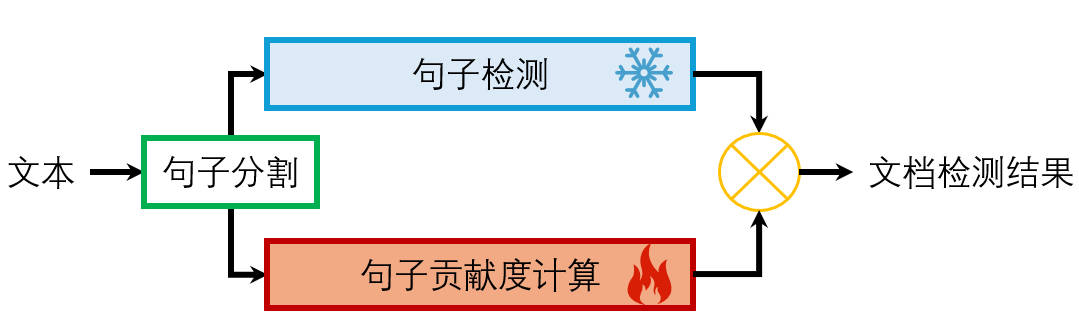
\includegraphics[width=0.9\textwidth]{figures/sent2arti.jpg}
    \caption{基于句子级文本检测技术的文档级文本检测方法}
    \label{fig:method-sent2arti}
\end{figure*}

为验证所提方法的优越性,本文也设计了系统的对比实验方案。基线模型包括三种典型架构:(1)直接迁移模型,将在句子级数据微调的 DeBERTa-V3-Large 模型直接应用于文档检测,用于验证领域适配性问题;(2)朴素加权模型,采用等权重策略(固定注意力值为1)处理所有句子,作为注意力机制有效性的对照基准;(3)长度加权模型,将句子长度作为权重系数,验证表面特征的有效性。所有对比模型均采用相同的训练/测试数据划分。

接下来将介绍基于句子级文本检测技术的文档级文本检测方法的三大模块,分别为句子分割模块、句子贡献度计算模块和句子检测模块。

\subsection{句子分割}

本节句子分割应用 \ref{sec:TOSWT-gen-sentence_splitter} 节中介绍的句子分割工具。这种分割方法能够将输入的文本字符串精准地分割成独立的句子,返回一个结构化的句子列表。其核心原理是通过一系列精心设计的正则表达式和逻辑规则来识别句子边界,有效处理各种复杂的标点符号和特殊情况。

该句子分割器的处理流程分为四个关键步骤。首先进行输入验证,检查输入文本是否为None或空字符串,确保对无效输入的优雅处理。其次,通过多个正则表达式规则在句子边界处插入换行符作为分隔符,这些规则涵盖了非句号结束标记、多重句号、标点符号后接引号或括号等多种复杂情况。然后,系统会进一步处理特殊标点情况,包括识别荣誉称谓、大写字母缩写和数字相关符号等,避免错误分割。最后,系统会清理文本中的多余空格和换行符,确保输出格式整洁。

\subsection{句子贡献度计算}

句子贡献度计算模块的设计旨在通过多头注意力机制捕获句子间的语义关联强度。该模块的核心思想是通过计算句子间的注意力权重,来评估每个句子在整体文本中的重要性和贡献度。句子列表 \( S = [s_1, s_2, \ldots, s_n]^T\) 经过句子贡献度计算模块后得到每一个句子的贡献度 \( \textbf{g} = [g_1, g_2, \ldots, g_n]^T\)。具体过程如图 \ref{fig:method-sent-contribution} 所示。

\begin{figure*}[htbp]
    \centering
    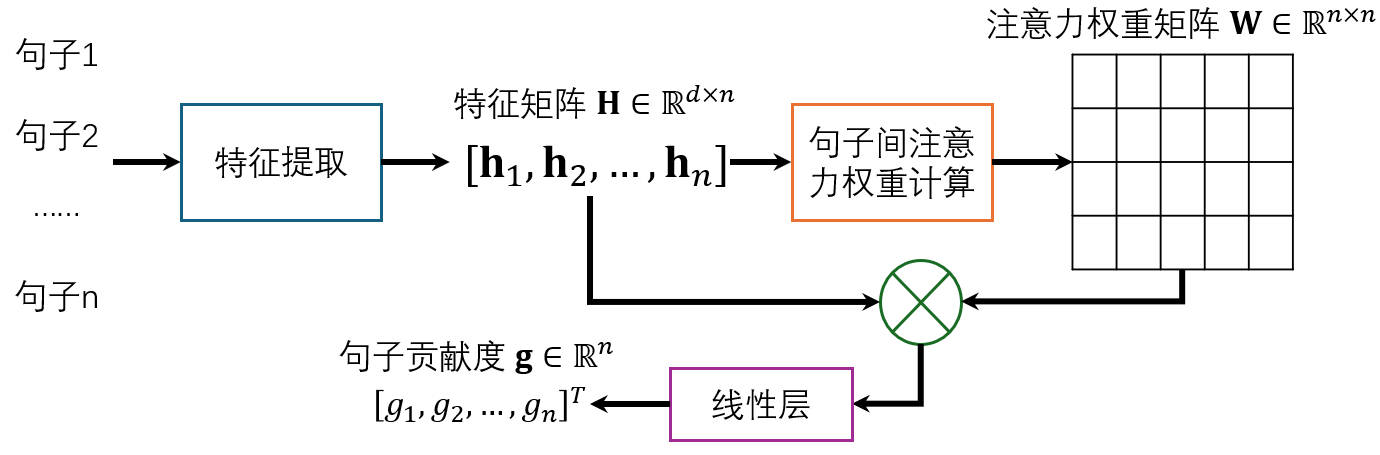
\includegraphics[width=\textwidth]{figures/sent-contribution.jpg}
    \caption{句子贡献度计算}
    \label{fig:method-sent-contribution}
\end{figure*}

具体而言,该模块先将每个句子特征提取:
\begin{equation}
\begin{aligned}
    \textbf{H} = \text{Feature\_Extract}(S)
\end{aligned}
\label{eq:method-sent-contribution-feature}
\end{equation}
其中, \(\textbf{H} \in \mathbb{R}^{d_\text{model} \times n}\) 为句子特征矩阵,\(S = [s_1, s_2, \ldots, s_n]^T\) 为句子列表。接着,计算句子间的注意力权重:
\begin{equation}
\begin{aligned}
    \textbf{W} = \text{Attention}(\textbf{H})
\end{aligned}
\label{eq:method-sent-contribution-attention}
\end{equation}
\(W \in \mathbb{R}^{n \times n}\) 为句子间的注意力权重矩阵。最后,通过特征矩阵 $\textbf{H}$ 与注意力权重矩阵 $\textbf{W}$ 做矩阵相乘运算后使用线性层降维,计算句子贡献度:
\begin{equation}
\begin{aligned}
    \textbf{g} = \text{Linear}(\textbf{HW})
\end{aligned}
\label{eq:method-sent-contribution}
\end{equation}
\(\textbf{g} \in \mathbb{R}^{n}\) 为句子贡献度向量。

在接下来的两节中,本文将详细介绍句子贡献度计算模块中的特征提取(公式 \ref{eq:method-sent-contribution-feature})和句子间注意力权重计算(公式 \ref{eq:method-sent-contribution-attention})的具体实现。

\subsubsection{特征提取}
\label{sec:method-sent2arti-featureextract}

特征提取模块使用BGE(Bidirectional Generative Encoder)\cite{bge_embedding} 作为基座模型。相比BERT,BGE采用RetroMAE非对称自编码架构,通过编码器-解码器的非对称设计强化语义表征能力。其中编码器(BERT-base)接受15-30\%掩码率的输入,专注于捕捉双向上下文;解码器仅使用单层Transformer 解码层,输入掩码率高达50-70\%,用于对遮掩文本进行重建。在训练过程中的编码阶段,模型对输入文本随机进行15\%-30\%的遮掩,然后通过编码得到对应文本的嵌入向量;而在解码阶段,为了提高任务复杂性,文本噪声被进一步加大(掩码比例增加至50\%-70\%),随后通过双流自注意力机制训练解码器从残缺信息中重建完整文本。相比 BERT 仅关注局部词语预测的架构,这种非对称设计能迫使编码器生成更加强大的嵌入向量,对提升模型的语义理解和表征能力效果显著。单个句子的特征提取三个阶段具体实现如图 \ref{fig:method-feature-extract} 所示。

\begin{figure*}[htbp]
    \centering
    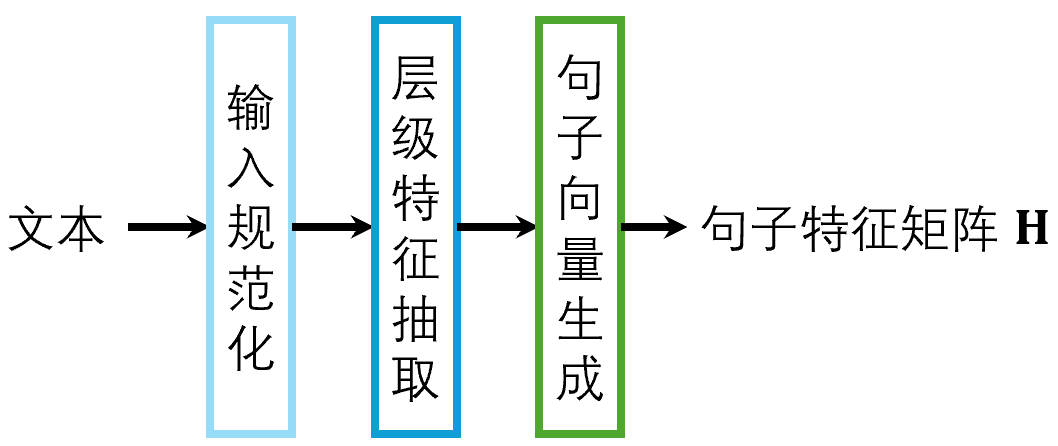
\includegraphics[width=0.6\textwidth]{figures/feature_extract.jpg}
    \caption{句子的特征提取}
    \label{fig:method-feature-extract}
\end{figure*}

特征提取模块中,单个句子$s_i$的编码主要分为以下三个阶段:

(1)阶段一:输入规范化

\textbf{分词与截断}:采用分词器对句子进行词切分后,生成对应token序列$[t_{i1}, t_{i2}, ..., t_{ik}]$(假设$s_i$分词后的token序列长度为$k$),然后对该序列执行动态填充(padding)与截断(truncation),确保最大序列长度不超过512。

\textbf{添加特殊标记}:在序列首尾分别添加 \texttt{[CLS]} 和 \texttt{[SEP]},形成规范化输入序列为 \( (\texttt{[CLS]}, t_{i1}, t_{i2}, \ldots, t_{ik}, \texttt{[SEP]}) \),其中 \(\texttt{[CLS]} \) 标记的隐藏状态作为全局语义表征将用于后续句子表征向量的生成。

(2)阶段二:层级特征抽取

\textbf{嵌入层映射}:通过三元嵌入组合(Token + Position + Segment)将离散输入映射为 768 维稠密向量。对$s_i$中每个位置 $j$ 的嵌入计算为:
\begin{equation}
    \textbf{E}_j = \textbf{E}_{token,j} + \textbf{E}_{pos,j} + \textbf{E}_{seg,j}, \quad j \in [1,k]
\end{equation}
其中,$\textbf{E}_{token,j}$ 表示词嵌入,$\textbf{E}_{pos,j}$ 表示绝对位置嵌入,$\textbf{E}_{seg,j}$ 表示段落嵌入。最终得到第 $i$ 个句子的嵌入矩阵$\textbf{E} \in \mathbb{R}^{k \times 768}$ 包含所有位置的联合表示,包括特殊标记\texttt{[CLS]} 和\texttt{[SEP]}。

\textbf{深度编码传播}:通过12层双向Transformer编码器对$s_i$的嵌入进行独立处理,逐步融入更深层次的语义。编码过程中第$l$层输出为:
\begin{equation}
    \textbf{H}^{(l)} = \text{LayerNorm}\left(\textbf{H}^{(l-1)} + \text{Attention}_\text{Transformer}(\textbf{H}^{(l-1)})\right)
\end{equation}
其中第一层的输入向量$\textbf{H}^0=\textbf{E}$,经过12层编码后最终得到句子$s_i$的上下文感知表示$\textbf{H}^{\text{final}} \in \mathbb{R}^{k \times 768}$。

(3)阶段三:句子向量生成

得到句子的层级特征之后,不同于直接提取首标记隐藏状态作为全局表征的做法,本模型采用混合池化策略提取每个句子的多模式特征以保留原始句子的细粒度语义。

具体来说,对于句子$s_i$,混合池化步骤需要分别计算其 $\texttt{[CLS]}$ 全局表征$\textbf{h}^\texttt{[CLS]}$($\texttt{[CLS]}$ 标记池化)、序列有效token部分的平均向量$\textbf{h}^\text{mean}$(均值池化)以及序列有效token部分沿特征维度的最大值$\textbf{h}^\text{max}$(最大池化),具体计算方式如下:
\begin{equation}
    \textbf{h}^\texttt{[CLS]} = \textbf{H}^{\text{final}}[0, :] \in \mathbb{R}^{768}
\end{equation}
\begin{equation}
    \textbf{h}^{\text{mean}} = \frac{1}{k} \sum_{j=1}^{k} \textbf{H}^{\text{final}}[j, :]
\end{equation}
\begin{equation}
    \textbf{h}^{\text{max}} = \max_{1 \leq j \leq k} (\textbf{H}^{\text{final}}[j, :])
\end{equation}

混合池化操作结束后还需要对语义向量与对应的混合池化表征进行投影降维。通过可学习的投影矩阵$\textbf{W}_p$将高维度混合特征映射至目标维度,最终得到单个句子的编码向量。整体计算流程如式\ref{sentence_embedding_generate}所示:
\begin{equation}\label{sentence_embedding_generate}
    \textbf{h} = \textbf{W}_p[\textbf{h}^\texttt{[CLS]}; \textbf{h}^{\text{mean}}; \textbf{h}^{\text{max}}] \in \mathbb{R}^d
\end{equation}
其中 $\textbf{W}_p \in \mathbb{R}^{d \times d_\text{hidden}}$ 为可学习参数矩阵,$d$ 为输出维度(默认768),$d_\text{hidden}$为投影维度。

\subsubsection{句子间注意力权重计算}

在 Transformer 中,定义注意力函数为输入为查询和一组键值,然后进行输出的函数,在此之中查询(Query, Q)、键(Key, K)、值(Value, V)和输出都是向量。在注意力函数中,简单地讲,输出实质上是值的加权和。此其中对于每个值的权重由权重相应的键以及查询计算得出。

本文中设计的句子间注意力权重计算过程参考了 Transformer 中的注意力机制 \cite{transformer} 并加以修改,其核心思想是通过计算查询与键之间的相似度来确定值的权重。在本文中,句子间注意力权重计算采用了单层基于稀疏掩码缩放点积注意力的多头注意力机制。以下是对这两种机制的详细介绍。

(1) 稀疏掩码缩放点积注意力

在 Transformer 论文中所采用的注意力机制为缩放点积注意力。该机制的输入由查询、键和值组成,其中查询和键的维度均为 \(d_k\),而值的维度为 \(d_v\)。在句子间注意力权重计算中,输入的查询、键和值都为句子特征矩阵 \(\textbf{H}\)。此外,基于语言学中句子关联性的距离衰减特性(即相邻句子通常具有更强的语义关联),本文在注意力机制中引入了稀疏掩码策略,具体通过设置距离阈值(distance threshold=3)来屏蔽远距离句子间的注意力交互。这种设计实现了两个关键优势:(1)符合文本的局部连贯性原理;(2)显著降低了长文档处理时的计算复杂度。

\begin{figure}[htbp]
	\centering
	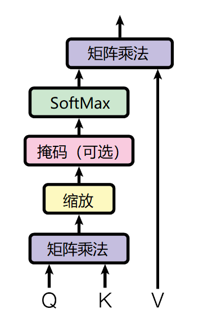
\includegraphics[scale = 0.4]{figures/DotAtt}
	\caption{稀疏掩码缩放点积注意力}
	\label{fig:DotAtt}
\end{figure}

在本文应用的稀疏掩码缩放点积注意力中,首先将句子特征矩阵 \( \textbf{H} \) 通过三个各不相同的线性层,再计算两个句子特征矩阵的乘积,并随后将矩阵乘法的结果除以系数 \(\sqrt{d_k}\)。再使用稀疏掩码遮掩距离过远的句子之间的注意力,接着,通过 softmax 函数后再与句子特征矩阵 \( \textbf{H} \) 做矩阵乘法,求出单次稀疏掩码缩放点积注意力。具体的过程如图 \ref{fig:DotAtt} 所示。

稀疏掩码缩放点积注意力函数的输出可以表示为:
\begin{equation}
\text{Attention}_\text{sparse}(\textbf{H}) = \text{SoftMax} \left( \frac{(\textbf{HW}^Q)(\textbf{HW}^K)^T}{\sqrt{d_k}} \odot \textbf{M} \right) (\textbf{HW}^V)
\label{eq3.1}
\end{equation}
其中,\(\textbf{M}\) 为稀疏掩码矩阵,\(\odot\) 表示遮蔽掩码操作。\(\textbf{W}^Q \in \mathbb{R}^{d_{\text{model}} \times d_k}\)、\(\textbf{W}^K \in \mathbb{R}^{d_{\text{model}} \times d_k}\)、\(\textbf{W}^V \in \mathbb{R}^{d_{\text{model}} \times d_v}\) 分别为图 \ref{fig:DotAtt} 中线性层 Q、线性层 K 和线性层 V 的权重矩阵。

(2) 多头注意力

本文为防止可能产生的模型性能下降问题,因此没有将键、值和查询的维度统一设定为 \(d_{\text{model}}\) 。在线性层中将查询、键和值分别投影为 \(d_k\)、\(d_k\) 和 \(d_v\) 维度。在此基础上,经过一系列操作生成 \(d_v\) 维的输出值。随后,将这些 \(d_v\) 维的输出值进行连接,并再次进行线性投影,以生成最终输出。具体过程如图 \ref{fig:MultiheadAtt} 所示。

\begin{figure}[htbp]
	\centering
	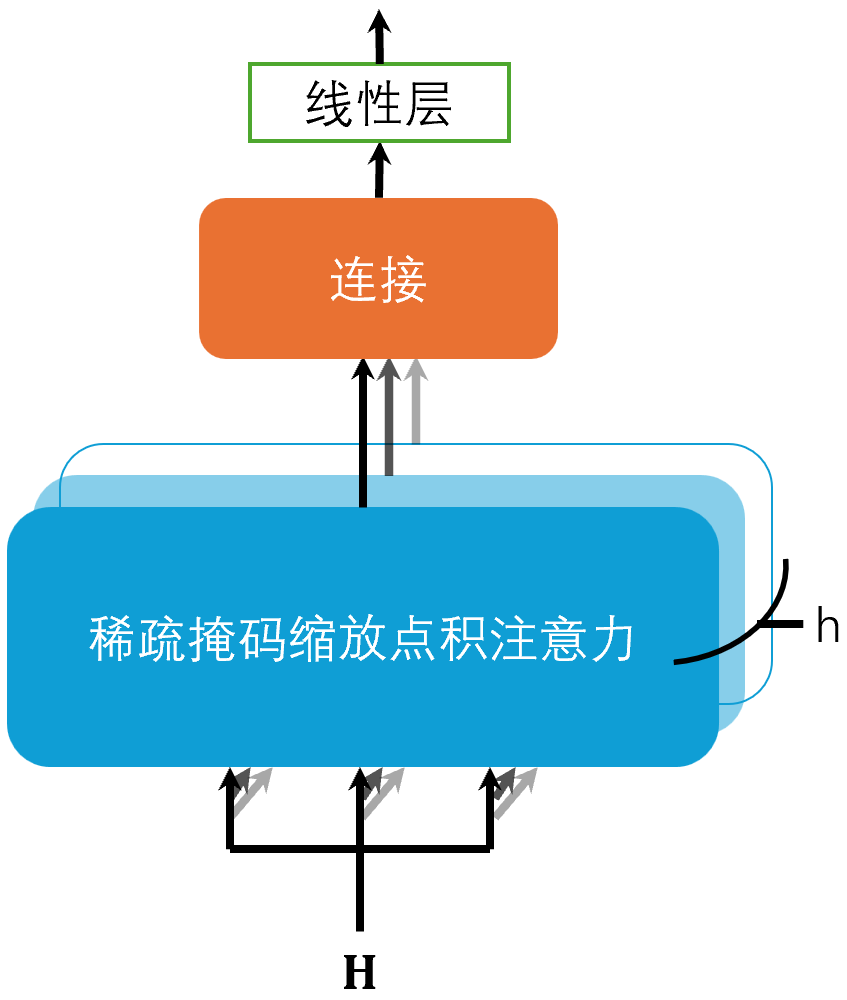
\includegraphics[scale = 0.4]{figures/MultiheadAtt}
	\caption{多头注意力 \cite{transformer}}
	\label{fig:MultiheadAtt}
\end{figure}

相较于单注意力头会导致信息的平均化,不同位置的信息可以被多头注意力同时关注。多头注意力机制的输出可以表示为:
\begin{equation}
\textbf{W} = \text{Attention}(\textbf{H}) = \text{Concat} \left(\text{Attention}_\text{sparse-1}(\textbf{H}), ..., \text{Attention}_\text{sparse-h}(\textbf{H}) \right)W^O
\label{eq3.2}
\end{equation}
在上述公式中,投影操作涉及的参数矩阵包括 \(\textbf{W}^Q \in \mathbb{R}^{d_{\text{model}} \times d_k}\)、\(\textbf{W}^K \in \mathbb{R}^{d_{\text{model}} \times d_k}\)、\(\textbf{W}^V \in \mathbb{R}^{d_{\text{model}} \times d_v}\) 以及 \(\textbf{W}^O \in \mathbb{R}^{hd_v \times d_{\text{model}}}\)。

在句子间注意力权重计算中,本文采用了 \(h = 8\) 个注意力头。\(d_k = d_v = d_{\text{model}} / h = 64\) 的维度赋予给了每一个注意力头。注意到,由于 \(d_k, d_v, d_{\text{model}} \) 被放缩,因此整体计算成本与具有全维度的单头注意力等价。

\subsection{句子检测}

句子检测模块旨在对单个句子的来源进行判断,具体框架如图 \ref{fig:sentence-classifier} 所示,主要包含三个组成部分,分别是:词嵌入层,特征提取器,以及分类器。

\begin{figure*}[htbp]
    \centering
    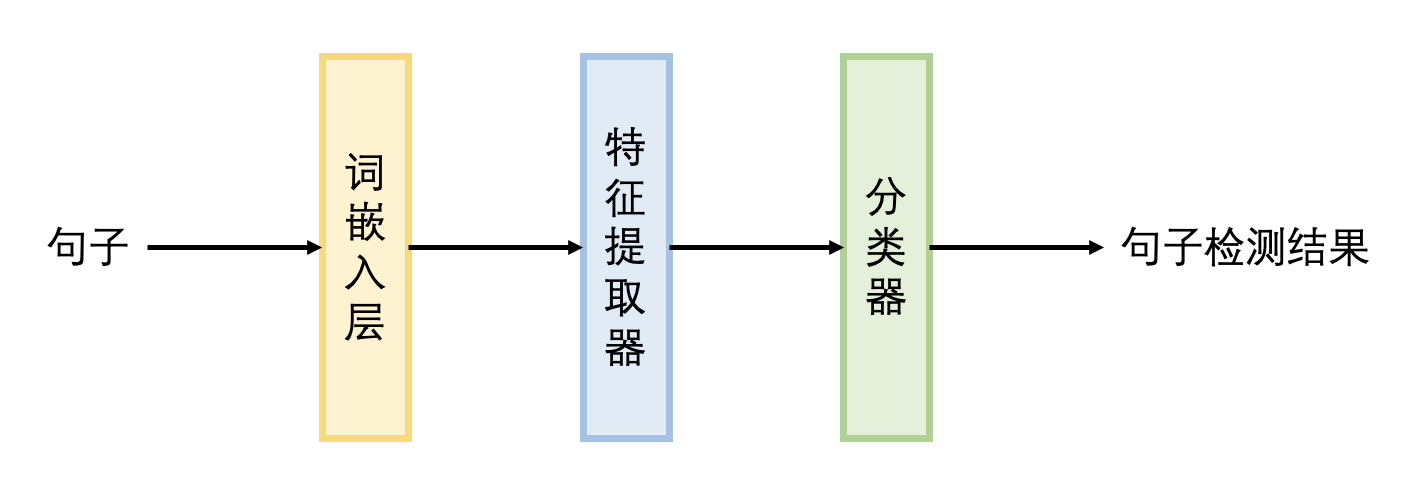
\includegraphics[width=0.9\textwidth]{figures/sentence-classifier.png}
    \caption{句子检测模块框架图}
    \label{fig:sentence-classifier}
\end{figure*}

给定一个待检测句子$S$,首先利用分词器对其进行词元化处理,表示为由$n$个词元$t_{i}$顺序排列组成的序列$[t_{1}, t_{2}, \ldots, t_{n}]$。本文采用的是DeBERTa-V3-Large对应的分词器,它会在每个序列前面自动添加一个$\texttt{[CLS]}$词元,用于整合整个序列语义,因此处理后的句子$S=[t_{0}, t_{1}, t_{2}, \ldots, t_{n}]$, $t_{0}$对应$\texttt{[CLS]}$词元。

将待检测句子$S$处理完毕后,利用句子检测模块对其进行检测。首先将其输入到词嵌入层$\mathrm{Embedding}(\cdot)$,将离散的词元转变为稠密的向量表示,便于后续利用神经网络进行特征提取,得到每个词元$t_{i}$对应的词嵌入表示$\mathbf{e}_{i}$:
\begin{equation}
    [\mathbf{e}_{0}, \mathbf{e}_{1}, \ldots, \mathbf{e}_{n}]=\mathrm{Embedding}([t_{0}, t_{1}, \ldots, t_{n}])
\end{equation}

为了挖掘句子的深层语义特征,利用预训练DeBERTa-V3-Large模型作为特征提取器,对句子进行特征表征,得到每个词元对应的隐层表征向量$\mathbf{h}_{i}$:
\begin{equation}
    [\mathbf{h}_{0}, \mathbf{h}_{1}, \ldots, \mathbf{h}_{n}]=\mathrm{DeBERTa}([\mathbf{e}_{0}, \mathbf{e}_{1}, \ldots, \mathbf{e}_{n}])
\end{equation}

由于在DeBERTa-V3-Large模型预训练过程中,$\texttt{[CLS]}$词元用于整合句子的全局语义信息,以往研究常常将其对应的隐层表征向量$\mathbf{h}_{0}$当做句子全局特征,用于下游的分类任务。本文沿用该方式,将$\texttt{[CLS]}$词元对应的隐层向量$\mathbf{h}_{0}$作为特征传入分类器,对句子进行检测。分类器由线性层$\mathrm{Linear}(\cdot)$和$\mathrm{SoftMax}(\cdot)$组成:
\begin{equation}
    \mathbf{p}=\mathrm{SoftMax}(\mathrm{Linear}(\mathbf{h}_{0}))
\end{equation}
其中,$\mathbf{p}$为模型的预测概率分布。

训练阶段,模型采用交叉熵损失函数来计算模型预测结果和实际标签之间的差异。利用句子级检测数据对本模块进行调优,能够有效捕捉文本中的细微差异和潜在模式,实现准确和可靠的句子级检测,为后续文档级文本检测提供坚实基础。在后续的模型设计中,该模块所有参数被冻结,不再参与整体模型参数的更新,从而节约计算成本。即便如此,模型整体性能并未受到过多影响,仍能实现较高的文档级检测准确率。

\section{实验}
\label{sec:method-experiment}

本文设计了如下实验,基于在第 \ref{chap:TOSWT} 章中介绍的模型改写文本检测数据集在句子、文档级数据上微调 \ref{sec:method-pretrain-roberta} 节中提及的 RoBERTa-Base 和 RoBERTa-Large 、在 \ref{sec:method-pretrain-deberta} 节中提及的 DeBERTa-V3-Base 和 DeBERTa-V3-Large 模型以及在 \ref{sec:method-sent2arti-featureextract} 中提及的 bge-base-en-v1.5 模型。以及在文档级数据微调实验中,使用 \ref{sec:method-sent2arti} 中提及的基于句子级文本检测技术的文档级文本检测方法。微调后再调用模型在测试集上输出预测标签,最后使用四种指标准确率(Accuracy)、精确率(Precision)、召回率(Recall)和 F1 分数评估预测标签的水准,进而评定微调后的模型能力。

本文所使用的预训练模型参数来源 URL 如表 \ref{tab:method-pretrain_model_url} 所示。

\begin{table*}[htbp]
\centering
\caption{预训练模型参数来源 URL} \label{tab:method-pretrain_model_url}
\begin{tabular}{ll}
\toprule
\textbf{模型}      & \textbf{来源 URL}                                                                 \\ \midrule
bge-base-en-v1.5 \cite{bge_embedding} & \url{https://huggingface.co/BAAI/bge-base-en-v1.5} \\ 
RoBERTa-Base \cite{liu_roberta_2019}     & \url{https://huggingface.co/FacebookAI/roberta-base}    \\
RoBERTa-Large \cite{liu_roberta_2019}   & \url{https://huggingface.co/FacebookAI/roberta-large}   \\
DeBERTa-V3-Base \cite{he2023debertav3improvingdebertausing}  & \url{https://huggingface.co/microsoft/deberta-v3-base}  \\
DeBERTa-V3-Large \cite{he2023debertav3improvingdebertausing} & \url{https://huggingface.co/microsoft/deberta-v3-large} \\ \bottomrule
\end{tabular}
\end{table*}

% 除了该对比实验外,我们还设计了消融实验,在 AES2 数据集评分基础上,进一步探索大语言模型改写文本的能力。有这样两个问题:原始文本对于大语言模型改写文本的影响有多大?大语言模型改写文本后,新文本的文本质量与原始文本质量一致性如何?为深入探索这两个问题,我们同样设计了两个额外的消融实验放置于 \ref{sec:method-experiment-analysis} 中。

\subsection{数据集设置}
\label{sec:method-experiment-dataset}

本实验中数据集采用在第 \ref{chap:TOSWT} 章中介绍的模型改写文本检测数据集。数据集示例如表 \ref{tab:TOSWT-eg} 所示,受单页篇幅所限,这里选取了一个包含两个句子的数据示例,该示例数据评分在其原始 AES2 数据集中被评定为 2 分。

\begin{table*}[htbp]
\BITSetup{ misc / tabularFontSize = 6}
\centering
\caption{模型改写文本检测数据集数据示例} \label{tab:TOSWT-eg}
\begin{tabular}{lp{12cm}}
\toprule
\multicolumn{1}{c}{\textbf{模型}} & \multicolumn{1}{c}{\textbf{文本}}  \\ \midrule
AES2 \cite{learning-agency-lab-automated-essay-scoring-2}                            & Luke think you should join the   seagoing cowboys program because you can travel all around and see some   pretty nice things like Luke it said in the passage that you take nine trips   to things like Greece,China,you will past the Atlantic Ocean and also you can   make the world a better place and you can be a hero for being nice. Also so if you want to you can help out animals in the passage it said, the   animals had to drink two or three times a day also a way you can help you   could clean the stalls on the ship and they will give you jobs and other   stuff and so you won't think it is boring you can have fun onboard to they   got a lot of things like baseball,and volleyball and the house it is   table-tennis tournaments,fencing,boxing,reading,whittling,and the games make   time go fast and that's why I think you should join the seagoing Cowboys   program. \\ \midrule
GPT3.5 \cite{chatgpt}                         & Luke thinks you should   join the Seagoing Cowboys program because you can travel all around and see   some pretty nice things. Like Luke said in the passage, you can take nine   trips to places like Greece and China. You will cross the Atlantic Ocean, and   you can make the world a better place by being nice and becoming a   hero. Also, if you want to, you can help out animals. In the passage, it said   that the animals had to drink two or three times a day. Another way you can   help is by cleaning the stalls on the ship. They will give you jobs and other   stuff. And so you won't think it's boring, you can have fun onboard too. They   have a lot of things like baseball, volleyball, table-tennis tournaments,   fencing, boxing, reading, and whittling. The games make time go fast, and   that's why I think you should join the Seagoing Cowboys program.   \\ \midrule
GPT4o \cite{gpt4o}                          & Luke believes you should join the seagoing   cowboys program because it allows you to travel extensively and see beautiful   places; as mentioned in the passage, you can undertake trips to destinations   like Greece and China, cross the Atlantic Ocean, and make the world a better   place while becoming a hero by being kind. Additionally, if you wish, you can assist with caring for animals; the   passage noted that the animals need to drink two or three times a day, and   one of the ways you can contribute is by cleaning the stalls on the ship,   where they will provide you with various tasks to keep you engaged, along   with fun activities such as baseball and volleyball, as well as other   pastimes like table tennis tournaments, fencing, boxing, reading, whittling,   which help make the time fly by-these are the reasons I think you should join   the seagoing Cowboys program. \\ \midrule
Gemini \cite{geminiteam2024geminifamilyhighlycapable}                         & Luke believes you should join   the Seagoing Cowboys program because it offers the opportunity to travel   extensively and witness beautiful sights, as he mentioned in the passage that   participants take nine trips to destinations like Greece and China, traverse   the Atlantic Ocean, and contribute to making the world a better place,   potentially becoming a hero through acts of kindness. Additionally, if you're interested, you can assist animals, as the passage   mentioned that they need to drink two or three times daily; you could also   help by cleaning stalls on the ship, and they'll provide you with various   tasks and activities to keep you engaged and prevent boredom, as there are   plenty of recreational options onboard, including baseball, volleyball, table   tennis tournaments, fencing, boxing, reading, whittling, all of which help   pass the time quickly, and that's why I believe you should consider joining   the Seagoing Cowboys program. \\ \midrule
Qwen \cite{qwen2025qwen25technicalreport}                           & Luke believes you should join   the seagoing cowboys program because it offers opportunities to travel   extensively and see beautiful places, such as Greece and China, as mentioned   in the passage. You will cross the Atlantic Ocean and contribute to making the   world a better place, thereby becoming a hero by being kind and   helpful. Additionally, if you wish, you can assist animals, as the passage notes   they need to drink two or three times a day. You could help by cleaning the   ship's stalls and taking on various jobs, ensuring the journey is enjoyable.   Onboard activities like baseball, volleyball, table tennis tournaments,   fencing, boxing, reading, and whittling make time pass quickly, which is why   I think you should join the seagoing cowboys program. \\ \midrule
DeepSeek \cite{deepseekai2024deepseekv3technicalreport}                       & Luke believes you should join   the seagoing cowboys program because it offers the opportunity to travel   extensively and witness beautiful sights, such as Greece and China, while   crossing the Atlantic Ocean, and it allows you to make the world a better place   and become a hero through kindness. Additionally, if you wish, you can assist animals, as mentioned in the   passage, which require drinking two or three times daily, and you can   contribute by cleaning the stalls on the ship, where they provide jobs and   other activities to ensure it's not boring; you can also enjoy onboard   entertainment like baseball, volleyball, table-tennis tournaments, fencing,   boxing, reading, whittling, and games that make time pass quickly, which is   why I recommend joining the seagoing cowboys program. \\ \bottomrule
\end{tabular}
\end{table*}

对于文档级数据,我们将模型改写文本检测数据集分割为训练集、验证集与测试集。这三个被分割后的小数据集在大数据集随机打乱后分别按照文档的个数以 $7:1:2$ 的比例分割出来。待微调的模型在训练集上微调过后,该模型在验证集上得到初步的模型效果,随后选取损失函数最低的模型在测试集上测试,进而得到最终的效果。

而句子级数据中关于数据集的分割步骤也与文档级数据的分割步骤类似。只不过第一步需要先将所有句子分割出来,单独打上标签,按照句子的个数随机打乱顺序后再以 $7:1:2$ 的比例分割为训练集、验证集和测试集。

对于词元个数过长的数据用例,我们将长度大于 512 后面的部分完全截断。不过,这一步是在词元化(tokenizer)的过程中处理的。

\subsection{实验参数设置}
\label{sec:method-experiment-parameter}

% 本章节所有实验均在配备NVIDIA TITAN RTX显卡(24GB显存)的高性能计算服务器上完成,服务器运行Ubuntu Linux 22.04 LTS操作系统。为保障实验环境的可重复性,我们详细记录了硬件配置和软件环境参数:服务器基础配置信息如表 \ref{tab:os-env} 所示;显卡详细规格参数(包括CUDA版本、驱动版本等)如表 \ref{tab:gpu-env} 所列;实验代码基于Anaconda搭建的Python 3.12.8虚拟环境执行,其中关键依赖库(如PyTorch、Transformers等)的具体版本信息详见表 \ref{tab:python-env}。所有实验环境参数均经过严格测试验证,确保实验结果的可靠性和可复现性。

所有实验均运行于 Ubuntu Linux 22.04 服务器上。详细实验操作系统环境如表 \ref{tab:os-env} 所示。

\begin{table*}[h]
\centering
\caption{实验操作系统环境} \label{tab:os-env}
\begin{tabular}{ll}
\toprule
\textbf{字段}    & \textbf{值}                               \\ \midrule
内核版本           & 6.8.0-49-generic                         \\
构建环境           & buildd@lcy02-amd64-103                   \\
架构             & x86\_64 (64位)                             \\
编译器            & x86\_64-linux-gnu-gcc-12                  \\
编译器版本          & 12.3.0                                   \\
编译器来源          & Ubuntu 12.3.0-1ubuntu1\textasciitilde22.04             \\
链接器   (GNU ld) & GNU Binutils for Ubuntu 2.38             \\
构建编号           & \#49\textasciitilde22.04.1-Ubuntu                       \\
构建类型           & SMP (对称多处理) + PREEMPT\_DYNAMIC(动态抢占模式) \\
构建时间           & Wed Nov 6 17:42:15 UTC 2024              \\
发行版基础          & Ubuntu 22.04.1 LTS                       \\ \bottomrule
\end{tabular}
\end{table*}

本章节全部实验均在拥有 24GB 显存容量的 NVIDIA TITAN RTX 显卡上完成,该显卡详细环境如表 \ref{tab:gpu-env} 所示。

\begin{table*}[h]
\centering
\caption{实验显卡环境} \label{tab:gpu-env}
\begin{tabular}{ll}
\toprule
\textbf{字段} & \textbf{值}           \\ \midrule
GPU   型号    & NVIDIA TITAN RTX     \\
GPU   架构    & Turning              \\
显存容量        & 24GB                 \\
TDP   (功耗)  & 320W                 \\
驱动版本        & NVIDIA-SMI 560.35.03 \\
CUDA   版本   & 12.6                 \\ \bottomrule
\end{tabular}
\end{table*}

本章节实验在实现上基于 Anaconda 库中搭建的 Conda 虚拟环境运行 Python 代码,Python 环境中部分重要包版本号如表 \ref{tab:python-env} 所示。

\begin{table*}[htbp]
\BITSetup{ misc / tabularFontSize = 6}
\centering
\caption{实验 Python 环境部分重要包版本} \label{tab:python-env}
\begin{tabular}{cll}
\toprule
\textbf{分类}                  & \textbf{字段}       & \textbf{版本号} \\ \midrule
\multirow{28}{*}{基础}         & conda             & 24.9.2       \\
                             & Python            & 3.12.8       \\
                             & GCC               & 11.2.0       \\
                             & cuda-cudart       & 11.8.89      \\
                             & cuda-cupti        & 11.8.87      \\
                             & cuda-libraries    & 11.8.0       \\
                             & cuda-nvrtc        & 11.8.89      \\
                             & cuda-nvtx         & 11.8.86      \\
                             & cuda-runtime      & 11.8.0       \\
                             & cuda-version      & 12.6         \\
                             & ipython           & 8.30.0       \\
                             & json5             & 0.9.25       \\
                             & matplotlib        & 3.9.2        \\
                             & matplotlib-base   & 3.9.2        \\
                             & matplotlib-inline & 0.1.6        \\
                             & nltk              & 3.9.1        \\
                             & numpy             & 2.0.1        \\
                             & openai            & 1.52.1       \\
                             & pandas            & 2.2.3        \\
                             & pillow            & 11.0.0       \\
                             & pip               & 24.2         \\
                             & regex             & 2024.11.6    \\
                             & sentencepiece     & 0.2.0        \\
                             & scikit-learn      & 1.6.0        \\
                             & scipy             & 1.14.1       \\
                             & tensorboard       & 2.17.0       \\
                             & xlsxwriter        & 3.1.1        \\
                             & yaml              & 0.2.5        \\ \midrule
\multirow{6}{*}{Torch}       & pytorch           & 2.5.1        \\
                             & pytorch-cuda      & 11.8         \\
                             & pytorch-mutex     & 1.0          \\
                             & torchaudio        & 2.5.1        \\
                             & torchtriton       & 3.1.0        \\
                             & torchvision       & 0.20.1       \\ \midrule
\multirow{5}{*}{HuggingFace} & accelerate        & 1.2.1        \\
                             & datasets          & 3.2.0        \\
                             & evaluate          & 0.4.0        \\
                             & huggingface-hub   & 0.27.0       \\
                             & tokenizers        & 0.21.0       \\
                             & transformers      & 4.47.1       \\ \bottomrule
\end{tabular}
\end{table*}

在基础的文档级和句子级的数据实验中,我们使用 DeBERTa 和 RoBERTa 作为实验用的模型并微调了四种模型:RoBERTa-Base、RoBERTa-Large、DeBERTa-Base 和 DeBERTa-Large,可变超参数包括批大小(batch size, BS)、学习率(learning rate, LR)、权重衰减系数(weight decay, WD)。在所有实验中,学习率均采用余弦退火衰减算法,并使用 AdamW 算法作为优化器。超参数详见表 \ref{tab:hyper-parameters},其中,在句子级实验中,大尺寸模型如 RoBERTa-Large 和 DeBERTa-V3-Large 的超参数均经过广泛地搜索长时间实验才找到可以使模型拟合于数据的一组超参数。DeBERTa-V3-Large 由于其总参数量较大,为防止超出显卡显存,因此批大小相较其他实验的 16 个为一批较小,设置为 4 个为一批。

\begin{table*}[htbp]
\centering
\caption{对比试验微调超参数列表}
\label{tab:hyper-parameters}
\begin{tabular}{c|l|ccc}
\toprule
                          & \textbf{模型}   & \textbf{批大小} & \textbf{初始学习率} & \textbf{权重衰减系数} \\ \midrule
\multirow{5}{*}{文档级}   & bge-base-en-v1.5 \cite{bge_embedding} & 16                  & $10^{-5}$                & 0.01                  \\
                          & RoBERTa-Base \cite{liu_roberta_2019}     & 16                  & $10^{-5}$                & 0.01                  \\
                          & RoBERTa-Large \cite{liu_roberta_2019}    & 16                  & $10^{-5}$                & 0.01                  \\
                          & DeBERTa-V3-Base \cite{he2023debertav3improvingdebertausing}  & 16                  & $10^{-5}$                & 0.01                  \\
                          & DeBERTa-V3-Large \cite{he2023debertav3improvingdebertausing} & 4                   & $10^{-5}$                & 0.01                  \\ \midrule
\multirow{5}{*}{句子级}   & bge-base-en-v1.5 \cite{bge_embedding} & 16                  & $10^{-5}$                & 0.01                  \\
                          & RoBERTa-Base \cite{liu_roberta_2019}     & 16                  & $10^{-5}$                & 0.01                  \\
                          & RoBERTa-Large \cite{liu_roberta_2019}    & 16                  & $10^{-6}$               & 0.0001                \\
                          & DeBERTa-V3-Base \cite{he2023debertav3improvingdebertausing}  & 16                  & $10^{-5}$                & 0.01                  \\
                          & DeBERTa-V3-Large \cite{he2023debertav3improvingdebertausing} & 4                   & $10^{-6}$               & 0.001                 \\ \midrule
句子级推测文档级 & 句子深度贡献度加权 & 16 & $10^{-5}$ & 0.01 \\ \bottomrule
\end{tabular}
\end{table*}

\subsubsection{交叉熵损失函数}

交叉熵函数 \cite{CrossEntropy} 是信息论和机器学习领域中的一个基本概念,主要用于量化两个概率分布之间的差异。其数学表达式为:对于真实分布 \( P \) 和预测分布 \( Q \),交叉熵 \( H(P, Q) \) 定义为:
\(
H(P, Q) = -\sum_x P(x) \log Q(x)
\)
。交叉熵反映了使用分布 \( Q \) 编码从分布 \( P \) 中抽取事件所需的平均比特数。当 \( Q \) 越接近于 \( P \) 时,交叉熵的值将趋向于减少。

在机器学习的应用中,交叉熵常常被用作分类任务的损失函数。例如,在本文讨论的六分类问题中,针对 \( m \) 个样本,该损失函数可以表示为:
\begin{align}
    L=-\frac{1}{m}\sum_{i=1}^m \sum_{j=1}^6 t_{ij}\log(y_{ij})
\end{align}
其中,\( t_{ij} \) 表示真实标签(采用 one-hot 编码),而 \( y_{ij} \) 则是模型的预测概率。这种损失函数设计能够有效地惩罚预测错误,尤其是在与 Softmax 或 Sigmoid 激活函数结合使用时,能够高效地计算梯度,并避免均方误差在学习过程中导致的学习速率下降问题。

交叉熵与信息熵及 KL 散度之间存在密切的关系。信息熵 \( H(P) \) 代表分布 \( P \) 的最佳编码长度,而交叉熵 \( H(P, Q) \) 则是使用分布 \( Q \) 编码 \( P \) 的代价。两者之间的差值即为 KL 散度,反映了两个分布之间的差异。在实际应用中,需要注意数值的稳定性,例如,通过对 \( Q(x) \) 进行裁剪以防止出现 \( \log(0) \) 的错误。

将交叉熵函数作为损失函数的优点在于其理论基础的严谨性与实践中的高效性。例如,在图像分类任务中,交叉熵直接优化预测概率与真实标签之间的匹配程度;而在本文所涉及的自然语言处理领域,它用于评估生成文本的概率分布的质量。

\subsubsection{AdamW 优化器}

AdamW 优化器 \cite{AdamW} 是对原始 Adam 优化器 \cite{Adam} 的一种重要改进,其算法流程如算法 \ref{algo:AdamW} 所示。该算法由 Ilya Loshchilov 和 Frank Hutter 于 2017 年提出,旨在解决传统 Adam 优化器在权重衰减(Weight Decay)处理方面的不足。在原始的 Adam 优化器中,权重衰减是通过将衰减项直接纳入梯度更新中来实现的。这种方法使得权重衰减的效果受到自适应学习率的影响,进而可能削弱正则化的有效性。相比之下,AdamW 优化器通过将权重衰减与梯度更新过程解耦,使其独立于梯度更新步骤,从而能够更准确地实现正则化效果。这一改进不仅提高了优化过程的稳定性,也增强了模型的泛化能力。

\begin{algorithm}[htb]
\caption{AdamW 优化算法} \label{algo:AdamW}
\begin{algorithmic}[1]
    \Require 学习率 $\psi(\text{lr})$, $\beta_1$, $\beta_2$ (betas), 初始参数 $\theta_0$ (params), 目标函数 $f(\theta)$ (objective), $\epsilon$, 权重衰减 $\chi$, amsgrad, maximize
    \Ensure $\theta_t$
    
    \State 初始化: $m_0 \leftarrow 0$ (一阶矩), $v_0 \leftarrow 0$ (二阶矩), $\widehat{v_0}^{max} \leftarrow 0$
    \For {$t = 1$ to $\ldots$}
        \If{maximize}
            \State $g_t \leftarrow - \nabla_\theta f_t(\theta_{t-1})$
        \Else
            \State $g_t \leftarrow \nabla_\theta f_t(\theta_{t-1})$
        \EndIf
        
        \State $\theta_t \leftarrow \theta_{t-1} - \psi \chi \theta_{t-1}$ \Comment{权重衰减}
        
        \State $m_t \leftarrow \beta_1 m_{t-1} + (1 - \beta_1) g_t$ \Comment{更新一阶矩}
        \State $v_t \leftarrow \beta_2 v_{t-1} + (1 - \beta_2) g_t^2$ \Comment{更新二阶矩}
        
        \State $\widehat{m_t} \leftarrow m_t / (1 - \beta_1^t)$ \Comment{偏差修正}
        \State $\widehat{v_t} \leftarrow v_t / (1 - \beta_2^t)$
        
        \If{amsgrad}
            \State $\widehat{v_t}^{max} \leftarrow \max(\widehat{v_{t-1}}^{\text{max}}, \widehat{v_t})$
            \State $\theta_t \leftarrow \theta_t - \psi \widehat{m}_t / (\sqrt{\widehat{v_t}^{\text{max}}} + \epsilon)$
        \Else
            \State $\theta_t \leftarrow \theta_t - \psi \widehat{m_t} / (\sqrt{\widehat{v_t}} + \epsilon)$
        \EndIf
    \EndFor
\end{algorithmic}
\end{algorithm}

AdamW 优化器的核心理念在于保留 Adam 优化器所具备的自适应学习率和动量机制,同时对权重衰减的处理方式进行改进。具体而言,AdamW 在参数更新过程中将权重衰减项独立于梯度计算,直接对参数施加衰减。这一方法显著增强了权重衰减的稳定性,有效防止了模型的过拟合现象,并提升了其泛化能力。实验结果表明,AdamW 在多种深度学习任务中均优于传统的 Adam 优化器,尤其在需要强正则化的情境下表现尤为突出。

AdamW 的优势体现在多个方面:首先,它提供了更为有效的正则化机制,从而更好地控制模型的复杂性;其次,在训练深度神经网络时展现出更为稳定的收敛性;最后,它适用于需要长时间训练的任务,如大语言模型(LLM)的预训练。然而,AdamW 也存在一些不足之处,例如对学习率和权重衰减系数的选择较为敏感,这要求进行更多的超参数调节,尤其在处理句子级别较大的模型时,调参工作显得尤为繁琐。

在实际应用中,AdamW 已成为多个深度学习框架(如 PyTorch)的默认优化器之一,特别适合于处理高维参数空间和复杂模型结构。其改进设计不仅保持了 Adam 的高效性,还进一步提升了模型的泛化性能,使其成为现代深度学习训练中的一项重要工具。

\subsubsection{余弦退火调度器}

余弦退火是一种在深度学习领域广泛应用的学习率调度策略,其核心理念是通过余弦函数的动态调整来优化模型的训练过程。该方法最早由 Ilya Loshchilov 和 Frank Hutter 在 2016 年提出的 SGDR 方法 \cite{SGDR} 中引入,随后迅速成为深度学习中的一项重要技术。余弦退火的名称源于其数学实现方式——学习率按照余弦函数曲线从初始值平滑下降至最小值,类似于金属加工中的退火过程,即先进行高温加热,随后缓慢冷却。

从数学原理的角度来看,余弦退火的公式为:
\begin{align}
\eta_t = \eta_{min} + \frac{1}{2}(\eta_{max} - \eta_{min})(1 + \cos(\frac{T_{cur}}{T_i}\pi))
\end{align}
其中,\(\eta_{max}\) 和 \(\eta_{min}\) 分别表示学习率的上限和下限,\(T_{cur}\) 是当前的训练步数,而 \(T_i\) 是总的训练步数。这一设计使得学习率在训练初期保持较高的值,以加速收敛,随后逐渐减小,从而便于模型对参数进行精细调整。与传统的阶梯式衰减或线性衰减方法相比,余弦退火提供了更为平滑的过渡,避免了学习率突变所引发的训练不稳定性。

在实际应用中,余弦退火展现出多重优势。首先,其周期性调整特性有助于模型跳出局部最优解,这对于处理多峰损失函数尤为有效。其次,该方法显著减少了人工调参的需求,通过预设的数学规律自动调整学习率,使其适用于各种复杂模型和大规模数据集。实验结果表明,在图像分类、自然语言处理等任务中,采用余弦退火策略的模型通常能实现更快的收敛速度和更优的泛化性能。例如,在 ImageNet 竞赛中,使用该策略的 ResNet 模型表现出了显著的性能提升。

\subsubsection{权重衰减算法}

权重衰减是一种在深度学习领域广泛应用的正则化技术,主要目的是防止模型出现过拟合现象。其基本原理是通过在损失函数中引入一个与权重参数的平方和成正比的惩罚项(即 \( L_2 \) 范数),以约束模型参数的大小。具体的数学表达式为:
\begin{align}
L' = L + \lambda \sum \theta_i^2
\end{align}
在此公式中,\( L \) 表示原始损失函数,\(\theta\) 是模型的权重,而 \(\lambda\) 是正则化系数,用于控制惩罚的强度。这样的设计使得模型在训练过程中更倾向于学习较小的权重值,从而降低模型的复杂度,避免对训练数据中噪声的过度敏感。

从实现机制的角度来看,权重衰减在梯度下降过程中直接影响参数的更新。以随机梯度下降为例,这一操作可以视为在每次迭代中对权重施加线性衰减,因此被称为“权重衰减”。需要指出的是,权重衰减通常不适用于偏置项,因为偏置主要负责输出的平移,对模型复杂性的影响相对较小。

权重衰减的作用机制可以从多个方面进行解释。首先,较小的权重使得模型对输入变化更加鲁棒,从而减少对噪声特征的依赖;其次,通过抑制特征之间的共线性,避免模型对某些特定特征组合的过度依赖;最后,它能够有效防止梯度爆炸问题,从而提升训练的稳定性。实验结果表明,在像 ImageNet 这样的大型数据集上,合理设置 \(\lambda\) 可以使测试误差降低 10\% 至 20\%。

在实际应用中,权重衰减常常与其他技术(如 Dropout 和批量归一化)结合使用。超参数 \(\lambda\) 的选择通常需要通过多次验证来确定,典型取值范围为 \(10^{-4}\) 到 \(10^{-2}\)。在本文中,我们经过多次测试确定了相应的权重衰减超参数。现代深度学习框架(如本文使用的 PyTorch)中内置了权重衰减功能,可以通过前述的 AdamW 优化器中的 weight\_decay 参数轻松启用。值得注意的是,尽管权重衰减与 \( L_2 \) 正则化在数学形式上相似,但其实现机制有所不同:前者直接修改优化过程,而后者则通过损失函数间接施加影响。

\subsection{评价指标}
\label{sec:method-experiment-metric}

本文共使用四种评价指标来评定,分别为\textbf{准确率}(Accuracy)、\textbf{精准率}(Precision)、\textbf{召回率}(Recall)和 \textbf{F1 分数}。这四种评价指标将在下面的小节中进行相应的介绍。由于模型改写文本检测本质上是多分类文本分类任务,因此后三者指标需要与二分类指标有相应变化。由于每个生成模型产生相同数量的文本,并且由于数据量对指标的影响最小,因此采用了对数据量敏感的宏观(macro)方法。

\subsubsection{准确率}

准确率(Accuracy)是机器学习中最基本且直观的分类评估指标,主要用于衡量模型整体预测的准确性。其核心定义为模型正确预测的样本数量占总样本数量的比例,数学表达式为:
\begin{align}
    Accuracy = \frac{TP+TN}{TP+TN+FP+FN}
\end{align}
在此公式中,\(TP\)(真正例)和 \(TN\)(真负例)分别表示正类和负类中预测正确的样本数量,而 \(FP\)(假正例)和 \(FN\)(假负例)则代表预测错误的样本数量。例如,在疾病诊断的场景中,如果模型成功识别了100名患者中的90名(包括健康和患病个体),则准确率为90\%,直观地反映了模型的综合判断能力。

\subsubsection{精准率}

精准率(Precision)是评估分类模型性能的重要指标之一,主要用于衡量模型预测为正类的样本中,实际为正类的比例。其数学定义为:
\begin{align}
    Precision = \frac{TP}{TP+FP}
\end{align}
在此公式中,\(TP\)(真正例)表示模型正确预测的正类样本数量,而 \(FP\)(假正例)则代表模型错误地将负类预测为正类的样本数量。该指标尤为关注模型预测为正类的可靠性。例如,在医疗诊断领域,高精准率意味着较少的健康患者被误诊为患病,从而避免不必要的治疗费用。

在本文的实验中,由于模型的文本改写检测本质上是一个多分类文本分类任务,因此精准率指标需要与二分类指标进行相应调整。考虑到每个生成模型产生相同数量的文本,并且数据量对指标的影响较小,因此采用了对数据量敏感的宏观(macro)方法进行评估。

\subsubsection{召回率}

召回率(Recall)是机器学习中用于评估分类模型性能的重要指标之一,主要用于衡量模型对正类样本的识别能力。其数学定义为:
\begin{align}
    Recall = \frac{TP}{TP+FN}
\end{align}
在此公式中,\(TP\)表示真正例,即模型正确预测的正类样本数量,而 \(FN\)则代表假负例,即实际为正类但被错误判定为负类的样本数量。该指标反映了所有真实正类样本中被模型成功识别的比例,因此也被称为“查全率”。在医疗诊断等高风险领域,高召回率意味着漏诊风险的降低。例如,如果癌症筛查模型的召回率达到90\%,则表明90\%的真实患者得到了正确检出。

在本文的实验中,由于模型的文本改写检测本质上属于多分类文本分类任务,因此召回率指标需要与二分类指标进行相应调整。考虑到每个生成模型产生相同数量的文本,并且数据量对指标的影响较小,因此采用了对数据量敏感的宏观(macro)方法进行评估。

\subsubsection{F1 分数}

F1分数是机器学习中评估分类模型性能的关键指标,它通过调和精确率(Precision)与召回率(Recall)来提供全面的性能评估。其计算公式为:
\begin{align}
    F1 = 2 \times \frac{Precision \times Recall}{Precision + Recall}
\end{align}
在此公式中,精确率用于衡量模型预测为正类的准确性(\(Precision = \frac{TP}{TP + FP}\)),而召回率则评估模型捕捉正类样本的能力(\(Recall = \frac{TP}{TP + FN}\))。这一设计使得F1分数对精确率与召回率赋予相同的重要性,任一指标的低下都会显著影响整体得分。

在本文的实验中,由于模型的文本改写检测本质上属于多分类文本分类任务,因此F1分数指标需要与二分类指标进行相应调整。考虑到每个生成模型产生相同数量的文本,并且数据量对指标的影响较小,因此采用了对数据量敏感的宏观(macro)方法进行评估。

\subsection{对比实验结果分析}
\label{sec:method-experiment-main}

本节通过两组对照实验系统评估了RoBERTa和DeBERTa模型在不同粒度文本理解任务中的表现。表 \ref{tab:document} 展示了文档级任务上的微调结果,其中DeBERTa-V3-Large以85.97\%的准确率和85.84\%的F1分数显著领先,验证了大规模预训练模型在处理长文本依赖关系时的优势。相比之下,表 \ref{tab:sentence} 揭示的句子级任务结果呈现出截然不同的特征:所有模型的绝对性能明显下降(最佳准确率仅49.61\%),且DeBERTa-V3-Base在精准率指标上意外超越其大型版本。这种差异凸显了文本处理粒度对模型性能的关键影响——文档级任务受益于丰富的上下文信息,而句子级任务则更依赖精准的局部语义理解。后续分析将深入探讨造成这种差异的内在机制,以及不同模型架构在两类任务中的适应性表现。

\subsubsection{句子级数据微调实验}

表 \ref{tab:sentence} 展示了RoBERTa和DeBERTa系列预训练语言模型在句子级自然语言处理任务上的微调性能对比。通过分析准确率(ACC)、精准率(P.)、召回率(R.)和F1分数四个关键评估指标,我们可以得出以下深入观察和结论。

\begin{table*}[htbp]
\caption{句子级数据上微调结果}
\centering
\begin{tabular}{l|cccc}
\toprule
\textbf{模型}& \textbf{准确率}   & \textbf{精准率}    & \textbf{召回率}    & \textbf{F1}   \\ \midrule
bge-base-en-v1.5  \cite{bge_embedding}   & 46.22          & 48.05          & 46.22          & 46.13          \\
RoBERTa-Base \cite{liu_roberta_2019}     & 45.08          & 50.13          & 45.08          & 43.93          \\
RoBERTa-Large \cite{liu_roberta_2019}    & 45.69          & 48.38          & 45.69          & 45.44          \\
DeBERTa-V3-Base \cite{he2023debertav3improvingdebertausing} & 47.76          & \textbf{51.49} & 47.76          & 46.93          \\
DeBERTa-V3-Large \cite{he2023debertav3improvingdebertausing} & \textbf{49.61} & 50.25          & \textbf{49.62} & \textbf{49.25} \\ \bottomrule
\end{tabular}
\label{tab:sentence}
\end{table*}

从整体性能表现来看,所有模型在句子级任务上的表现明显低于文档级任务(对比表 \ref{tab:document}),这反映了句子级理解任务固有的挑战性。DeBERTa-V3-Large依然保持领先地位,其准确率达到49.61\%,F1分数49.25\%,但相比文档级任务85.97\%的准确率有显著下降。这种性能差距凸显了句子级语义理解的复杂性,其中上下文信息有限,模型更难捕捉深层次的语义关系。

值得注意的是,DeBERTa-V3-Base在精准率指标上以51.49\%的表现超过所有其他模型,包括其大型版本DeBERTa-V3-Large(50.25\%)。这一反常现象可能表明,在句子级任务中,基础规模的DeBERTa模型在避免假阳性预测方面具有特殊优势。同时,RoBERTa系列的表现相对较弱,RoBERTa-Large的准确率仅为45.69\%,甚至低于DeBERTa-V3-Base的47.76\%,这说明在句子级任务中,模型架构的改进比单纯增加参数规模更为重要。

深入分析各指标之间的关系可以发现,所有模型的精准率都高于召回率,这与文档级任务中的观察一致,但差距更为显著。RoBERTa-Base的精准率(50.13\%)比召回率(45.08\%)高出5.05个百分点,DeBERTa-V3-Base的差距更是达到3.73个百分点(51.49\% vs 47.76\%)。这种系统性偏差表明,当前预训练语言模型在句子级任务中普遍倾向于保守预测,可能为了避免错误而牺牲了部分正类样本的识别能力。

从模型规模的影响来看,RoBERTa从Base到Large版本的性能提升非常有限,准确率仅增加0.61个百分点(45.08\%到45.69\%),F1分数增加1.51个百分点(43.93\%到45.44\%)。相比之下,DeBERTa从Base到Large版本的提升更为明显,准确率增加1.85个百分点(47.76\%到49.61\%),F1分数增加2.32个百分点(46.93\%到49.25\%)。这一对比强烈表明,在句子级任务中,DeBERTa的架构设计能够更有效地利用增加的模型容量。

特别值得注意的是各模型在F1分数上的表现。作为精准率和召回率的调和平均,F1分数更好地反映了模型的整体分类能力。DeBERTa-V3-Large以49.25\%的F1分数领先,其次是DeBERTa-V3-Base的46.93\%,两者都明显优于RoBERTa对应版本。这一差距说明DeBERTa的分离注意力机制和增强的位置解码设计特别适合处理句子级的语义关系建模。

从实际应用角度考虑,这些结果提供了重要启示。在句子级任务中,DeBERTa-V3-Base可能是性价比最高的选择,它在多个指标上接近甚至超过更大规模的模型,同时计算成本更低。此外,所有模型相对较低的绝对性能分数(均低于50\%)表明,当前的预训练语言模型在句子级理解任务上仍有很大改进空间,可能需要开发专门的架构改进或训练策略。

这些实验结果也提出了若干值得深入研究的问题。首先,为什么DeBERTa-V3-Base在精准率上表现最佳?这是否与其基础规模的参数配置和特定注意力模式的交互有关?其次,为什么模型规模扩大带来的性能提升在句子级任务中不如文档级任务显著?这可能反映了句子级和文档级任务对模型能力的不同需求。最后,如何解释所有模型在句子级任务中表现出的更大的精准率-召回率差距?这可能与句子级数据的特性或评估方式有关。

综上所述,表 \ref{tab:sentence} 通过详实的实验数据,揭示了预训练语言模型在句子级任务中的性能特点和局限。这些发现不仅对模型选择有直接指导意义,也为未来研究指明了改进方向,包括开发更适合句子级理解的架构变体、设计更有效的微调策略,以及深入理解不同粒度文本处理任务的本质差异。这些见解将有助于推动自然语言处理技术在句子级理解任务上的进一步发展。

\subsubsection{文档级数据微调实验}

表 \ref{tab:document} 详细展示了RoBERTa和DeBERTa两个主流预训练语言模型家族在文档级自然语言处理任务上的微调性能对比结果。通过对准确率(Accuracy)、精准率(Precision)、召回率(Recall)和F1分数四个核心评估指标的全面分析,我们可以得出若干重要发现。

\begin{table*}[htbp]
\caption{文档级数据上微调结果}
\centering
\begin{tabular}{l|cccc}
\toprule
\textbf{模型}& \textbf{准确率}   & \textbf{精准率}    & \textbf{召回率}    & \textbf{F1}   \\ \midrule
bge-base-en-v1.5 \cite{bge_embedding} & 73.24          & 74.21          & 73.24          & 73.04          \\
RoBERTa-Base \cite{liu_roberta_2019}  & 72.88          & 77.26          & 72.89          & 72.73          \\
RoBERTa-Large \cite{liu_roberta_2019} & 80.92          & 81.84          & 80.92          & 80.55          \\
DeBERTa-V3-Base \cite{he2023debertav3improvingdebertausing} & 79.85          & 81.44          & 79.85          & 79.81          \\
DeBERTa-V3-Large \cite{he2023debertav3improvingdebertausing} & \textbf{85.97} & \textbf{86.31} & \textbf{85.96} & \textbf{85.84} \\ \midrule
DeBERTa-V3-Large\cite{he2023debertav3improvingdebertausing}(Sentence)  & 78.11 & 80.63 & 78.11 & 77.87 \\
朴素加权 & 76.27 & 81.19 & 76.27 & 76.02 \\
长度加权 & 77.85 & 81.18 & 77.85 & 77.65 \\
句子深度贡献度加权 & \uline{78.97} & \uline{82.00} & \uline{78.97} & \uline{78.74} \\ \bottomrule
\end{tabular}
\label{tab:document}
\end{table*}

从整体性能趋势来看,所有评估指标都呈现出明显的层级结构:DeBERTa-V3-Large以显著优势领先,其准确率达到85.97\%,精准率86.31\%,召回率85.96\%,F1分数85.84\%,这四项指标均明显优于其他对比模型。这一结果验证了模型规模和架构改进的双重重要性。值得注意的是,DeBERTa-V3-Base(79.85\%准确率)与RoBERTa-Large(80.92\%准确率)的性能相当接近,这表明DeBERTa系列在基础模型规模下就能达到与更大规模RoBERTa模型相近的性能水平,充分体现了其架构设计的先进性。

深入分析模型架构的影响可以发现,DeBERTa系列采用的分离注意力机制和增强型掩码解码器带来了显著优势。特别是在精准率指标上,DeBERTa-V3-Base(81.44\%)已经超过了RoBERTa-Large(81.84\%),而DeBERTa-V3-Large更是将这一优势扩大到86.31\%。这表明DeBERTa的架构改进特别有利于提升模型预测的精确性,减少假阳性错误的发生。这一特性在需要高精度预测的应用场景(如医疗诊断或金融风险评估)中尤为重要。

从模型规模的角度观察,RoBERTa从Base到Large版本的性能提升幅度为8.04个百分点(准确率从72.88\%到80.92\%),而DeBERTa从Base到Large版本的提升幅度更大,达到6.12个百分点(从79.85\%到85.97\%)。虽然绝对提升值略低,但考虑到DeBERTa-Base的起点更高,这一相对提升仍然非常可观。这证实了增加模型参数规模对性能提升的持续有效性,同时也表明在优质架构设计的基础上,扩大模型规模能带来更显著的效果。

特别值得注意的是各模型在精准率和召回率之间的平衡关系。所有模型的精准率都略高于召回率,这种系统性差异可能反映了当前预训练语言模型在文档级任务中普遍存在的保守预测倾向。RoBERTa-Base的精准率(77.26\%)比召回率(72.89\%)高出4.37个百分点,这一差距在更大规模的模型中有所缩小,DeBERTa-V3-Large的精准率(86.31\%)仅比召回率(85.96\%)高出0.35个百分点。这表明随着模型规模和架构的优化,模型在保持高精确性的同时,也能更好地覆盖正类样本,实现更均衡的性能表现。

F1分数的变化趋势进一步验证了上述发现。作为精准率和召回率的调和平均数,F1分数综合反映了模型的整体分类性能。DeBERTa-V3-Large的F1分数达到85.84\%,比RoBERTa-Large的80.55\%高出5.29个百分点,这一提升幅度超过了准确率的提升(5.05个百分点),说明DeBERTa的优势在综合考虑精确性和全面性时更为明显。

在句子特征融合策略的比较中,本文提出的句子深度贡献度加权机制以78.97\%的准确率表现最佳,比朴素加权方法提高了 2.70 个百分点,同时对比直接将文本输入句子级检测模型,完成了其指标的全面提升。长度加权方法也取得了不错的效果,F1值达到 77.65\%,说明文本长度这一特征确实能带来性能提升。然而,所有句子级特征融合策略的表现都明显低于完整文档级建模的DeBERTa-V3-Large模型,这突显了文档级整体建模的重要性。

从实际应用的角度来看,这些结果对模型选择具有重要指导意义。在计算资源允许的情况下,DeBERTa-V3-Large显然是首选方案;在资源受限时,DeBERTa-V3-Base能以较小的参数量达到与RoBERTa-Large相当的性能,是更经济高效的选择。此外,精准率普遍高于召回率的现象提示我们,在这些模型的工业部署中可能需要根据具体应用场景的需求,通过调整分类阈值来优化精确性或召回率。

这些实验结果也为未来研究指明了若干方向。首先,DeBERTa架构的成功验证了分离注意力机制在文档级任务中的有效性,值得进一步研究和扩展。其次,模型规模扩大带来的性能提升尚未达到平台期,暗示继续增大模型规模可能仍有潜力。最后,精准率和召回率之间的不平衡现象值得深入分析,可能需要设计专门的损失函数或训练策略来改善。

综上所述,表 \ref{tab:document} 通过系统的对比实验,不仅展示了不同预训练语言模型在文档级任务上的性能差异,更为模型架构设计、规模选择和实际应用提供了重要的实证依据。这些发现将有助于研究人员和工程师在文档级自然语言处理任务中做出更明智的模型选择和应用决策。

\section{消融实验}
\label{sec:method-experiment-ablative}

本节在文档级文本检测任务上,设计若干消融实验以探究不同模型架构对文本改写检测性能的影响。

\subsection{消融实验设置}
\label{sec:method-experiment-ablative-design}

为探究本文提出架构中不同模块对于文本改写检测性能的影响,本文设计了多组消融实验。具体而言,本文主要关注以下问题:(1)句子贡献度对于文本改写检测性能的影响;(2)句子深度贡献度方法中句子间注意力模块对文本改写检测性能的影响;(3)句子深度贡献度方法中掩码机制对文本改写检测性能的影响。为此,本文设计了以下消融实验:

\textbf{朴素句子贡献度}:使用朴素的句子贡献度计算方法对比,其中包括上文提及的朴素加权及词元长度加权等方法。

\textbf{双塔模型}:分别采用 BGE 模型和 RoBERTa-Large 模型作为句子贡献度计算模块,得出句子贡献度后与句子检测模块的结果进行加权融合,得到最终的文本改写检测结果。与最终的句子深度贡献度方法相比,双塔模型的主要区别在于没有句子间注意力权重计算模块。

\textbf{句子深度贡献度}:即本文提出的句子深度贡献度方法,分别采用 BGE 模型和 RoBERTa-Large 模型作为句子贡献度计算模块中的特征提取模块。

\textbf{句子深度贡献度无掩码}:与句子深度贡献度方法相比,句子深度贡献度无掩码方法在计算句子间注意力权重时不使用掩码机制。该实验主要用于验证稀疏掩码机制对文本改写检测性能的影响。

消融实验超参数如表 \ref{tab:ablative-parameter} 所示。由于单张 24 GB 显存显卡容量有限,因此不同模型的批大小设置不同。RoBERTa-Large 模型和句子深度贡献度方法中使用的 RoBERTa-Large 模型均采用 8 的批大小,BGE 模型和句子深度贡献度方法中使用的 BGE 模型均采用 16 的批大小,句子深度贡献度方法中使用的 RoBERTa-Base 模型采用 4 的批大小。初始学习率和权重衰减系数经网格搜索确定。

\begin{table*}[htbp]
\centering
\caption{消融实验超参数设置}
\label{tab:ablative-parameter}
\begin{tabular}{l|ccc}
\toprule
                      & \textbf{批大小} & \textbf{初始学习率} & \textbf{权重衰减系数} \\ \midrule
$\text{双塔模型}_\text{RoBERTa-Large}$    & 8            & $10^{-6}$      & 0.001           \\
$\text{双塔模型}_\text{BGE}$         & 16           & $10^{-5}$      & 0.01            \\
$\text{句子深度贡献度}_\text{RoBERTa-Large}$ & 4            & $10^{-6}$      & 0.001           \\
句子深度贡献度无掩码            & 16           & $10^{-5}$      & 0.01            \\
句子深度贡献度               & 16           & $10^{-5}$      & 0.01           \\ \bottomrule
\end{tabular}
\end{table*}

\subsection{消融实验结果}
\label{sec:method-experiment-ablative-result}

消融实验结果如表 \ref{tab:ablative-result} 所示。前三行中 DeBERTa-V3-Large 是在句子级数据直接微调后在文档级数据上测试;朴素加权是将每个句子检测后的结果简单加权;长度加权是以句子词元个数与句子检测后的结果加权。

\begin{table*}[htbp]
\centering
\caption{消融实验结果}
\label{tab:ablative-result}
\begin{tabular}{l|cccc}
\toprule
                           & \textbf{准确率}   & \textbf{精准率}   & \textbf{召回率}   & \textbf{F1}    \\ \midrule
DeBERTa-V3-Large \cite{he2023debertav3improvingdebertausing} (Sentence) & 78.11          & 80.63          & 78.11          & 77.87          \\
朴素加权                        & 76.27          & 81.19          & 76.27          & 76.02          \\
长度加权                        & 77.85          & 81.18          & 77.85          & 77.65          \\ \midrule
$\text{双塔模型}_\text{RoBERTa-Large}$ & 78.26          & 81.86          & 78.26          & 78.09          \\
$\text{双塔模型}_\text{BGE}$          & 78.70          & \textbf{82.08} & 78.71          & 78.54          \\
$\text{句子深度贡献度}_\text{RoBERTa-Large}$ & 77.64          & 81.87          & 77.64          & 77.48          \\
句子深度贡献度无掩码            & 78.61          & 81.61          & 78.61          & 78.35          \\ \midrule
句子深度贡献度                  & \textbf{78.97} & 82.00          & \textbf{78.97} & \textbf{78.74} \\ \bottomrule
\end{tabular}
\end{table*}

消融实验结果表格系统地展示了不同模型架构在文档级文本检测任务上的性能表现,通过对比分析可以得出几个重要结论。首先观察基准方法的表现,直接使用句子级微调的DeBERTa-V3-Large模型在文档级测试中取得了78.11\%的准确率和77.87\%的F1值,这为后续方法提供了性能基准。朴素加权方法表现最弱,F1值仅为76.02\%,说明简单的等权重融合策略效果有限。长度加权方法F1值提升到77.65\%,表明考虑句子长度这一特征能带来一定改进,但提升幅度仍然有限。

在双塔模型对比部分,实验结果显示出明显的架构优势。使用RoBERTa-Large的双塔模型F1值达到78.09\%,已经超过所有基准方法。而采用BGE模型的双塔模型表现更优,F1值提升至78.54\%,其精准率更是达到82.08\%的最高值。这一结果表明双塔结构能有效捕捉句子级特征,帮助句子检测模块提升性能。与此同时BGE模型在句子特征提取方面可能比RoBERTa-Large更具优势。

注意力机制的分析结果特别值得关注。句子深度贡献度无掩码版本相比完整版F1值下降了0.39个百分点,验证了掩码机制的有效性。值得注意的是,使用RoBERTa-Large的句子深度贡献度方法表现反而不如双塔模型,F1值降至77.48\%,这可能说明该架构对基座模型的选择较为敏感,或者RoBERTa-Large在注意力计算中存在过拟合问题。

最终完整的句子深度贡献度方法在所有评估指标上都取得最佳表现,准确率达到78.97\%,F1值达到78.74\%。相比表现次优的BGE双塔模型,其召回率提升0.26个百分点,说明该方法在保持高精准率的同时,对正例的覆盖更全面。这一结果充分证实了本文提出的句子深度贡献度方法的有效性,特别是其结合双塔结构和注意力机制的设计优势。各项指标的均衡提升表明,该方法能够较好地建模文档级文本特征,实现更准确的改写检测。

\section{本章小结}
\label{sec:method-conclusion}

本章系统地研究了基于预训练语言模型的文本改写检测方法,通过对比实验和消融分析,深入探讨了不同模型架构在文档级和句子级文本检测任务中的表现差异。主要研究内容和结论总结如下:

在模型架构方面,本章详细分析了 RoBERTa 和 DeBERTa 系列模型的技术特点。实验结果表明,DeBERTa-V3-Large 在文档级任务中表现最优,准确率达到 85.97\%,显著优于其他对比模型。这验证了其解耦注意力机制和增强掩码解码器在处理长文本依赖关系时的优势。值得注意的是,DeBERTa-V3-Base 以较小的模型规模达到了接近 RoBERTa-Large 的性能水平,体现了架构创新的重要性。除此之外,提出了一种基于句子级文本检测技术的文档级文本检测方法,采用了句子深度贡献度加权来融合句子级特征,取得了较好的效果。这一方法在文档级任务中表现出色,准确率达到 78.97\%,为后续研究提供了新的思路。

在任务粒度方面,研究发现文档级和句子级任务呈现出不同的性能特征。所有模型在文档级任务上的表现明显优于句子级任务,这反映了丰富的上下文信息对模型性能的积极影响。特别地,在句子级任务中,模型规模扩大带来的性能提升相对有限,而架构差异的影响更为显著,这为不同应用场景下的模型选择提供了重要参考。

然而,研究也揭示了当前方法的一些局限性。首先,模型在测试集上的性能下降表明泛化能力仍需提升;其次,句子级任务的整体性能偏低(最佳准确率仅49.61\%)说明现有方法在细粒度语义理解方面仍有改进空间;最后,在探索性数据分析实验中,被改写文本与原文质量一致性实验仍需改进。

这些发现为后续研究指明了多个方向:在文本质量一致性实验中开发更鲁棒的评估模型以提高跨数据集一致性;设计专门针对句子级任务的改进架构;探索更精细的评估指标来捕捉文本改写的多维特性。同时,实验结果也为实际应用中的模型选择提供了实证依据,特别是在需要权衡计算成本和性能表现的场景中。

总的来说,本章通过系统的实验设计和深入的分析,为模型改写文本检测领域提供了重要的方法学参考和技术基础,以推动相关技术在教育质量评估等实际应用中的发展。
%%==================================================
%% chapter01.tex for BIT Master Thesis
%% modified by pinren lu
%% version: 0.1
%% last update: Dec 25th, 2016
%%==================================================
% 第五章 模型改写文本检测系统设计与实现

% 1. 需求分析
% 2. 系统设计
% 3. 系统实现
% 4. 系统展示
% 5. 本章小结

\chapter{模型改写文本检测系统设计与实现}
\label{chap:sys}

本章主要介绍基于模型改写文本检测系统的设计与实现,第三、四章从理论和实验方面验证了本文提出方法的有效性,为了进一步验证方法在实际应用场景中的有效性,本文以提出的模型改写文本检测方法为基础,遵循软件开发过程的基本原则,设计并实现了模型改写文本检测系统,涵盖文本改写和检测模型改写两大文本生成功能。通过该系统,可以进一步提升文本改写的流畅性与多样性、检测模型改写的准确性。本章以需求分析、系统设计、系统实现以及系统功能展示四个部分介绍模型改写文本检测系统。

\section{需求分析}
\label{sec:sys-need}

本研究所提出的模型改写文本检测系统为自然语言处理领域提供了一种创新的技术解决方案,显著增强了对学生写作文本是否经过AI改写的检测能力。该系统旨在为用户提供一个功能全面、性能卓越的文本改写检测平台,能够满足多样化的文本改写需求,并提供精准的模型文本改写检测服务。接下来,将从业务需求和功能需求的角度对该系统进行详细分析。

\subsection{业务需求分析}
\label{sec:sys-bus-need}

随着人工智能技术的迅速进步,文本改写及其检测的需求日益增加。尤其在教育领域,教师迫切需要评估和反馈学生的写作,而学生则希望借助改写工具来提升自己的写作能力。因此,本文提出的模型改写文本检测系统应满足以下业务需求:

(1)\textbf{高质量文本改写服务:} 系统应能够提供优质的文本改写服务,以帮助用户提升文本的流畅性和多样性;
(2)\textbf{准确的模型改写检测服务:} 系统应具备准确识别文本是否经过模型改写的能力,以便教师有效评估学生的写作水平;
(3)\textbf{用户友好的界面设计:} 系统应提供简洁明了的用户界面,以便用户轻松操作;
(4)\textbf{卓越的性能与稳定性:} 系统应具备出色的性能和稳定性,以处理大量文本数据;
(5)\textbf{数据安全与隐私保护:} 系统应确保用户数据的安全性,并提供隐私保护措施,以防止数据泄露;
(6)\textbf{良好的可扩展性:} 系统应具备良好的可扩展性,以支持根据需求进行功能的扩展与升级;
(7)\textbf{多平台兼容性:} 系统应能够在多种平台上运行,包括桌面和移动设备;
(8)\textbf{实时反馈机制:} 系统应提供实时的文本改写与检测反馈,帮助用户及时了解文本质量和改写效果;
(9)\textbf{用户管理功能:} 系统应具备用户管理功能,支持用户注册、登录及权限管理等操作。

\subsection{功能需求分析}
\label{sec:sys-func-need}

本文从用户与管理员两个视角对系统功能进行了全面分析,以深入理解不同用户身份下的需求与功能要求。在用户功能需求分析中,重点关注系统所提供的各项服务与功能,包括用户注册、登录、文本改写和检测功能,以及用户历史信息的管理。这些功能旨在确保用户能够顺利使用系统并获得良好的使用体验。在管理员功能需求分析方面,重点则放在系统的管理与维护功能上,包括用户管理、功能管理、模型管理以及文本改写信息的管理。这些功能的设计旨在确保系统高效、稳定地运行,并能够及时处理用户反馈与相关问题。通过这样的分析,能够更全面地满足不同用户群体的需求。

\begin{figure*}[htb]
    \centering
    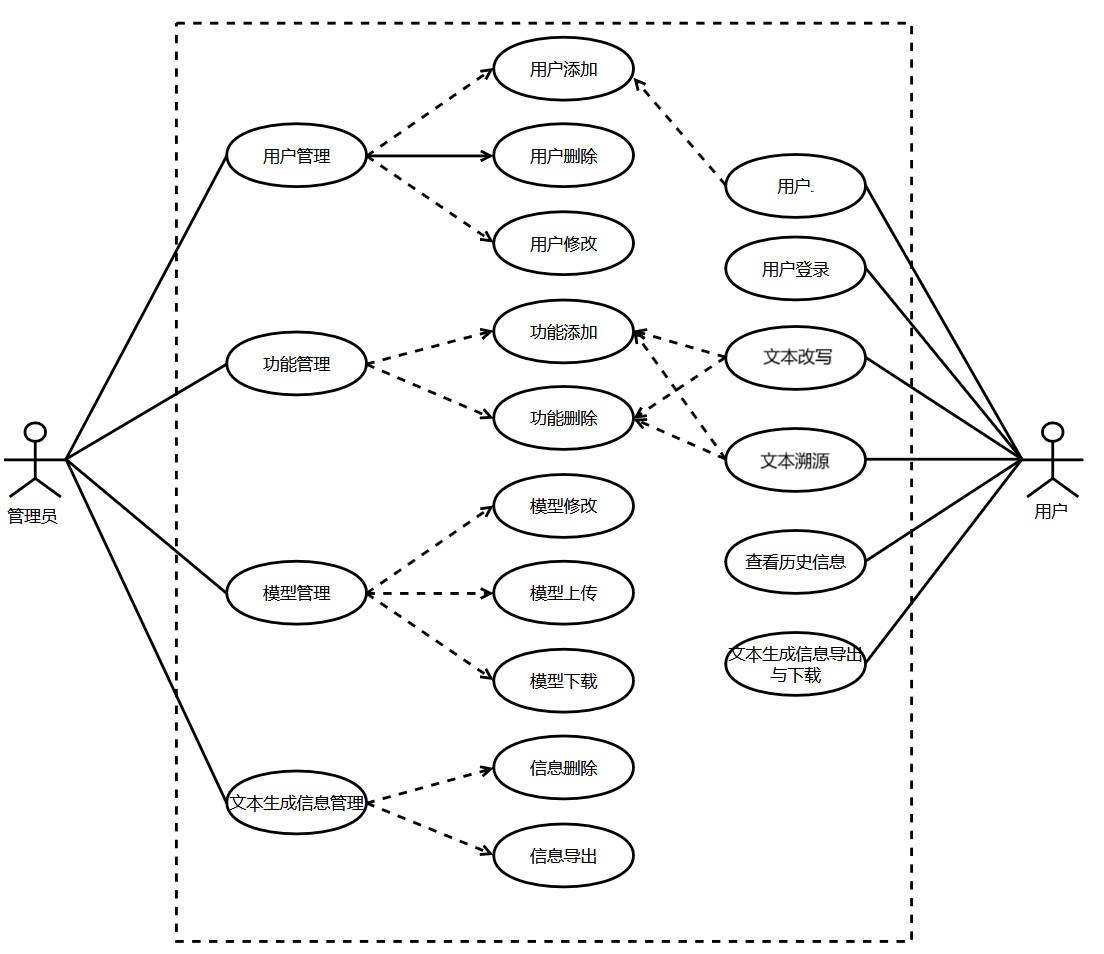
\includegraphics[width=\textwidth]{figures/sys-use-case.jpg}
    \caption{模型改写文本检测系统用例图}
    \label{fig:sys-use-case}
\end{figure*}

模型改写文本检测系统的总体用例图如图 \ref{fig:sys-use-case} 所示。

本系统的用户功能需求分析如下:

(1)\textbf{用户注册}:系统允许用户自主进行注册,以便创建个人账户;(2)\textbf{用户登录}:用户可凭借已注册的账号和密码成功登录系统;(3)\textbf{文本改写服务}:系统应为用户提供文本改写服务,能够根据用户输入的文本进行润色,使其更加流畅和通顺;(4)\textbf{文本溯源服务}:系统应提供检测服务,以判断某段文本是否经过改写或由人工智能生成,依据输入的源文本得出相应的检测结果;(5)\textbf{查看历史信息}:用户可以通过历史信息查询接口查看以往的改写记录和检测结果;(6)\textbf{文本生成信息导出与下载}:支持用户将文本信息导出并下载至本地存储。

本系统的管理员功能需求分析如下:

(1)\textbf{用户管理}:管理员可对用户进行添加、删除及信息修改等管理操作;
(2)\textbf{功能管理}:系统支持功能的扩展,允许管理员添加新功能或删除不必要的功能;
(3)\textbf{模型管理}:管理员可以通过模型管理接口进行模型的修改、上传和下载;
(4)\textbf{文本生成信息管理}:管理员负责对系统内冗余的文本信息进行删除或导出操作。

\section{系统设计}
\label{sec:sys-design}

本章主要介绍模型改写文本检测系统的架构设计、模块和接口设计以及相关信息的数据库存储设计。

\subsection{系统架构设计}
\label{sec:sys-arch}

为增强系统的灵活性、可扩展性与可维护性,本系统采用了前后端分离的架构设计。在该架构中,前端主要负责接收用户输入数据并发送相应的系统反馈,而后端则承担具体的服务提供和处理逻辑,并将处理结果反馈至前端。系统的整体架构如图 \ref{fig:sys-arch} 所示,涵盖表现层、应用层、持久层及基础层。

\begin{figure*}[htb]
    \centering
    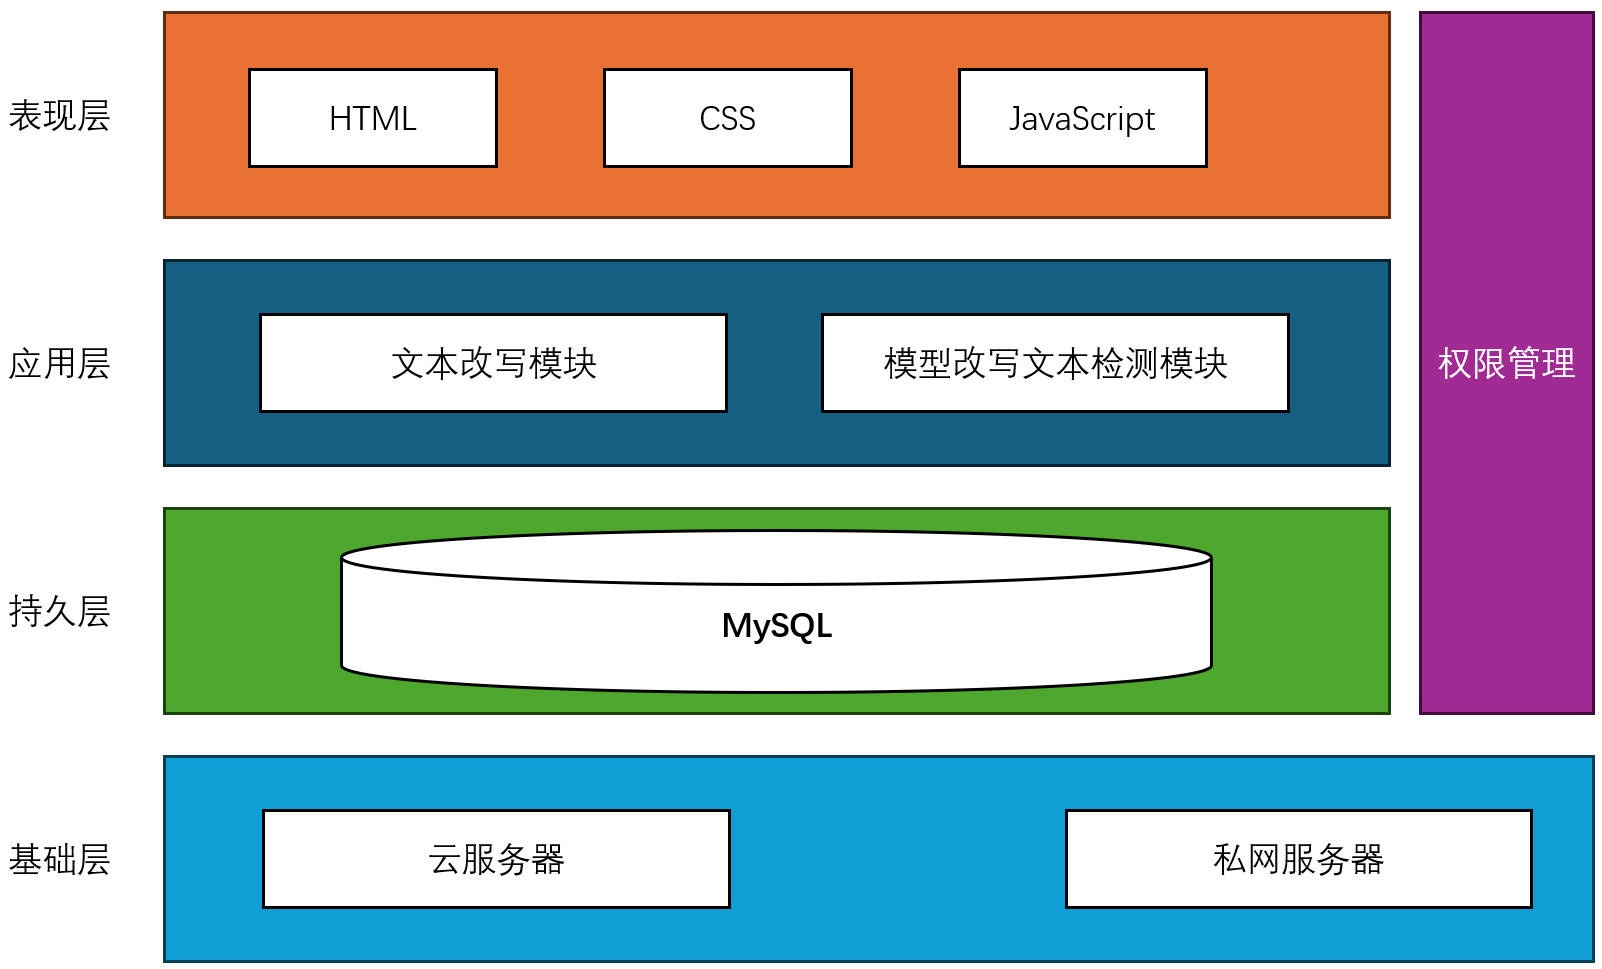
\includegraphics[width=\textwidth]{figures/sys-architecture.jpg}
    \caption{模型改写文本检测系统架构设计}
    \label{fig:sys-arch}
\end{figure*}

(1)\textbf{表现层}:该层负责处理用户界面的逻辑与交互控制,管理界面的逻辑和权限设置,以用户友好的方式展示系统数据并实现用户交互。其内容涵盖用户界面设计、页面布局及组件设计、样式设计与美化。该层通过 HTML 定义页面结构,利用 CSS 进行样式美化,并通过 JavaScript 处理页面交互及动态效果。

(2)\textbf{应用层}:此层包含系统的核心业务逻辑,包括对话生成模块和机器翻译模块,同时提供用户管理及管理员管理服务。将业务逻辑独立设置于应用层,有助于不同功能模块的开发、测试和部署的独立性与灵活性,从而便于后续功能的扩展与升级。

(3)\textbf{持久层}:该层负责系统的数据存储与访问管理,使用 MySQL 存储用户账户信息、个人资料、权限与角色信息以及用户活动记录等结构化数据。同时,利用 MongoDB 存储生成的文本内容等非结构化信息。通过独立的数据层,系统的数据访问变得更加统一与安全,同时也便于数据的管理与维护。

(4)\textbf{基础层}:该层通过云服务器和私有网络服务器进行系统部署,提供必要的基础运行环境。

通过采用前后端分离的系统架构,本系统能够实现前后端的松耦合、功能模块化
和独立部署,提高了系统的灵活性、可扩展性和可维护性,同时也提高了开发效率。

\subsection{模块和接口设计}
\label{sec:sys-module}

模型改写文本检测系统的结构可分为用户模块、系统管理模块和系统功能模块
% ,模块之间的关系如图 \ref{fig:sys-module} 所示
。用户模块的主要功能包括用户的注册与登录,允许用户创建账户、进行密码管理,并提供身份验证与授权功能,以确保用户能够顺利访问和使用系统服务。系统管理模块则专注于功能管理、模型管理和数据管理,支持对系统功能的灵活扩展,管理员可以通过该模块添加新功能或移除不再需要的功能。此外,模型管理接口允许对系统模型进行修改、上传和下载,而数据管理功能则负责管理文本生成信息,用户可以通过系统接口删除冗余文本信息或将其导出至本地。系统功能模块是系统的核心部分,提供多种具体的系统服务,以处理前端接收的请求。系统功能涵盖文本改写和文本检测等,通过此模块,用户可以与系统进行交互,发起特定请求或执行特定任务。系统根据接收到的请求,调用相应的功能模块进行处理,并生成相应的响应。

% \begin{figure*}[htb]
%     \centering
%     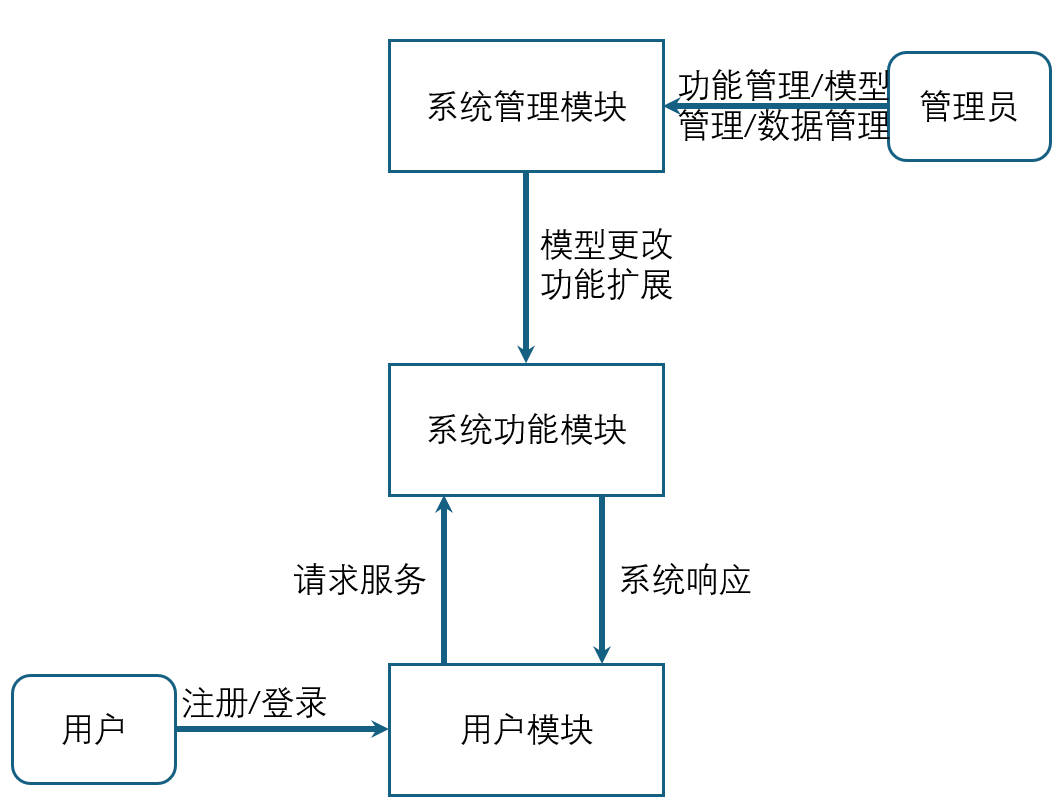
\includegraphics[width=0.8\textwidth]{figures/sys-module.jpg}
%     \caption{模型改写文本检测系统模块设计}
%     \label{fig:sys-module}
% \end{figure*}

为了实现系统对用户的服务以及系统内不同模块之间数据传输,本章定义了系统核心接口,如表 \ref{tab:sys-interfaces} 所示,其中展示了模型改写文本检测系统核心接口及所属模块。

\begin{table*}[htb]
    \centering
    \caption{模型改写文本检测系统核心接口及所属模块说明}
    \label{tab:sys-interfaces}
    \begin{tabular}{ccl}
        \toprule
        \textbf{接口名} & \textbf{所属模块} & \textbf{接口描述} \\
        \midrule
        userRegister & 用户模块 & 接收用户提交注册信息,并进行用户注册。 \\
        userLogin & 用户模块 & 接收用户提交登录信息,并进行身份验证和授权。 \\
        getModelInfo & 系统管理模块 & 查询系统提供的模型,返回相关模型信息。 \\
        upLoadModel & 系统管理模块 & 用于上传已训练好的模型到系统中,以供后续的服务需求。 \\
        downLoadModel & 系统管理模块 & 用于从系统中导入已有模型。 \\
        funcDelete & 系统管理模块 & 用于删除系统中不需要的功能。 \\
        funcCreate & 系统管理模块 & 用于扩展系统功能,提供更好的服务。 \\
        dataManage & 系统管理模块 & 用于管理系统中的文本生成信息,支持删除或下载文本数据。 \\
        polishService & 系统功能模块 & 接收用户输入,使用模型进行文本改写,并返回结果。 \\
        detectService & 系统功能模块 & 接收用户输入,使用模型进行模型改写文本检测,并返回结果。 \\
        \bottomrule
    \end{tabular}
\end{table*}

\subsection{数据库设计}
\label{sec:sys-db}

根据系统的存储需求,本文选择使用 MySQL 数据库来存储结构化数据,具体包括用户表、功能表、模型表和文本数据表等。

MySQL 数据库的设计主要涵盖用户表、功能表、模型表以及文本数据表。每个表均设有相应的字段和数据类型,以满足系统的特定需求。

用户表用于记录用户的相关信息,包括用户 ID、用户名、密码、邮箱、权限、注册时间以及最近登录时间等,具体结构如表 \ref{tab:user-table} 所示。

\begin{table*}[htb]
    \centering
    \caption{用户表} \label{tab:user-table}
    \begin{tabular}{ccccc}
        \toprule
        \textbf{序号} & \textbf{字段} & \textbf{数据类型} & \textbf{说明} & \textbf{是否主键} \\
        \midrule
        1 & user\_id & int & 用户 ID & 是 \\
        2 & user\_name & varchar(30) & 用户名 & 否 \\
        3 & password & varchar(128) & 密码 & 否 \\
        4 & email & varchar(30) & 邮箱 & 否 \\
        5 & authority & enum & 权限 & 否 \\
        6 & register\_time & datetime & 注册时间 & 否 \\
        7 & lat\_login\_time & datetime & 最近登录时间 & 否 \\
        \bottomrule
    \end{tabular}
\end{table*}

功能表用于记录系统中各项相关功能的信息,具体包括功能 ID、功能名称及其对应的功能接口,详细结构如表 \ref{tab:func-table} 所示。

\begin{table*}[htb]
    \centering
    \caption{功能表} \label{tab:func-table}
    \begin{tabular}{ccccc}
        \toprule
        \textbf{序号} & \textbf{字段} & \textbf{数据类型} & \textbf{说明} & \textbf{是否主键} \\
        \midrule
        1 & fuc\_id & int & 功能 ID & 是 \\
        2 & fuc\_name & varchar(30) & 功能名称 & 否 \\
        3 & fuc\_interface & varchar(30) & 功能接口 & 否 \\
        \bottomrule
    \end{tabular}
\end{table*}

模型表用于存储与系统内模型相关的信息,涵盖模型 ID、模型名称、模型类型以及模型的上传时间等内容。具体结构详见表 \ref{tab:model-table}。

\begin{table*}[htb]
    \centering
    \caption{模型表} \label{tab:model-table}
    \begin{tabular}{ccccc}
        \toprule
        \textbf{序号} & \textbf{字段} & \textbf{数据类型} & \textbf{说明} & \textbf{是否主键} \\
        \midrule
        1 & model\_id & int & 模型 ID & 是 \\
        2 & model\_name & varchar(20) & 模型名称 & 否 \\
        3 & model\_type & varchar(20) & 模型类型 & 否 \\
        4 & model\_size & varchar(20) & 模型大小 & 否 \\
        5 & upload\_time & datetime & 上传时间 & 否 \\
        \bottomrule
    \end{tabular}
\end{table*}

文本数据表旨在记录与用户及模型改写文本相关的信息,具体包括用户 ID、文本 ID、操作类型、操作时间以及文本内容等。该表的详细结构如表 \ref{tab:text-table} 所示。

\begin{table*}[htbp]
    \centering
    \caption{文本数据表} \label{tab:text-table}
    \begin{tabular}{ccccc}
        \toprule
        \textbf{序号} & \textbf{字段} & \textbf{数据类型} & \textbf{说明} & \textbf{是否主键} \\
        \midrule
        1 & user\_id & int & 用户 ID & 是 \\
        2 & text\_id & int & 文本 ID & 是 \\
        3 & text\_type & varchar(20) & 操作类型 & 否 \\
        4 & generated\_time & datetime & 操作时间 & 否 \\
        5 & text\_content & text & 文本内容 & 否 \\
        \bottomrule
    \end{tabular}
\end{table*}

\section{系统实现}
\label{sec:sys-implement}

本节将详细介绍模型改写文本检测系统所使用的工具和系统服务,并对系统功能进行模块化阐述。

\subsection{开发环境与工具}
\label{sec:sys-env}

本研究采用前后端分离的架构进行系统开发。前端部分利用 Vue 框架构建用户界面,以提供优良的交互体验。后端则基于 Pytorch 和 Transformers 等技术,负责文本生成服务的构建。在编程语言的选择上,前端和后端分别使用 HTML、CSS、JavaScript 和 Python,以满足不同开发需求。为提升开发效率,选用 Vscode 作为主要开发工具。在数据存储方面,系统采用 MySQL 数据库,以存储用户信息及生成的文本数据。为简化后端业务逻辑的处理,使用 Flask 框架。此外,为确保系统的安全性,采用 JWT 技术进行权限管理和用户身份验证。本文所使用的所有开发环境和工具的详细信息见表 \ref{tab:sys-env}。

\begin{table*}[htbp]
    \centering
    \caption{模型改写文本检测系统开发环境与工具}
    \label{tab:sys-env}
    \begin{tabular}{cc}
        \toprule
        \textbf{描述} & \textbf{配置} \\
        \midrule
        编程语言 & HTML、CSS、JavaScript、Python \\
        前端框架 & Vue \\
        服务端开发 & Pytorch1.8、Transformers \\
        开发工具 & Vscode \\
        数据库 & MySQL \\
        权限管理 & JWT \\
        服务器端 & Flask1.1.2、Docker \\
        \bottomrule
    \end{tabular}
\end{table*}

鉴于管理员仅能在系统后台通过脚本执行管理操作,本文将重点展示用户端的系统功能。用户端主要包括用户注册与登录、文本改写、检测模型改写以及历史信息查询等功能。用户注册与登录功能旨在允许用户创建账户并访问系统;文本改写功能则用于对用户输入的文本进行改写;检测模型改写功能用于验证输入文本是否经过模型处理;历史信息查询功能则帮助用户检索其过往操作记录。

\subsection{用户注册与登录}

用户可以通过已注册的账号和密码登录系统,相关界面如图 \ref{fig:sys-login} 所示。在用户注册过程中,需填写用户名、密码和电子邮箱等信息,系统将对所输入的信息进行验证,以确保其合法性和完整性。如果用户尚未注册账户,可以通过注册页面进行注册,具体界面如图 \ref{fig:sys-register} 所示。

\begin{figure*}[htb]
    \subfloat[listentry][用户登录]{
        \label{fig:sys-login}
        \centering
        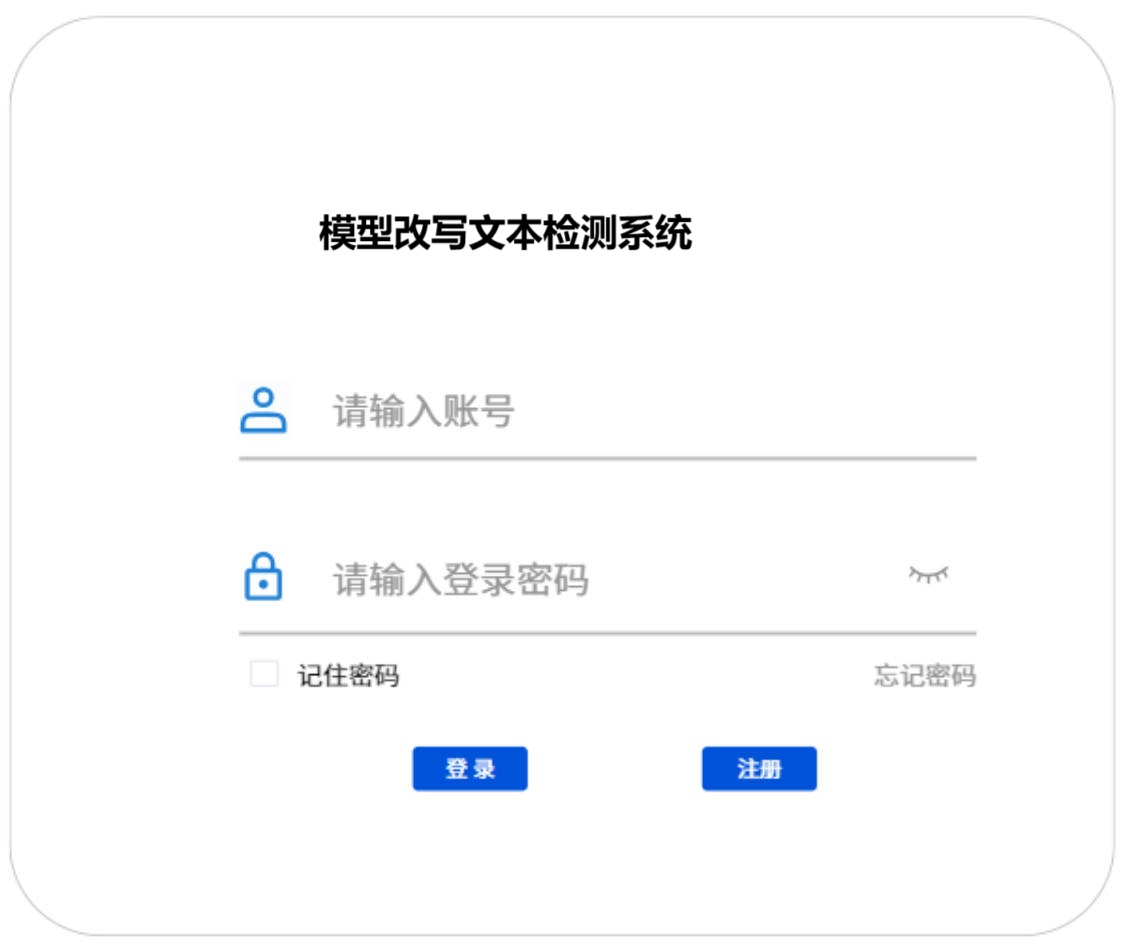
\includegraphics[width=0.45\textwidth]{figures/sys-login.jpg}
    }
    \hfill
    \subfloat[listentry][用户注册]{
        \label{fig:sys-register}
        \centering
        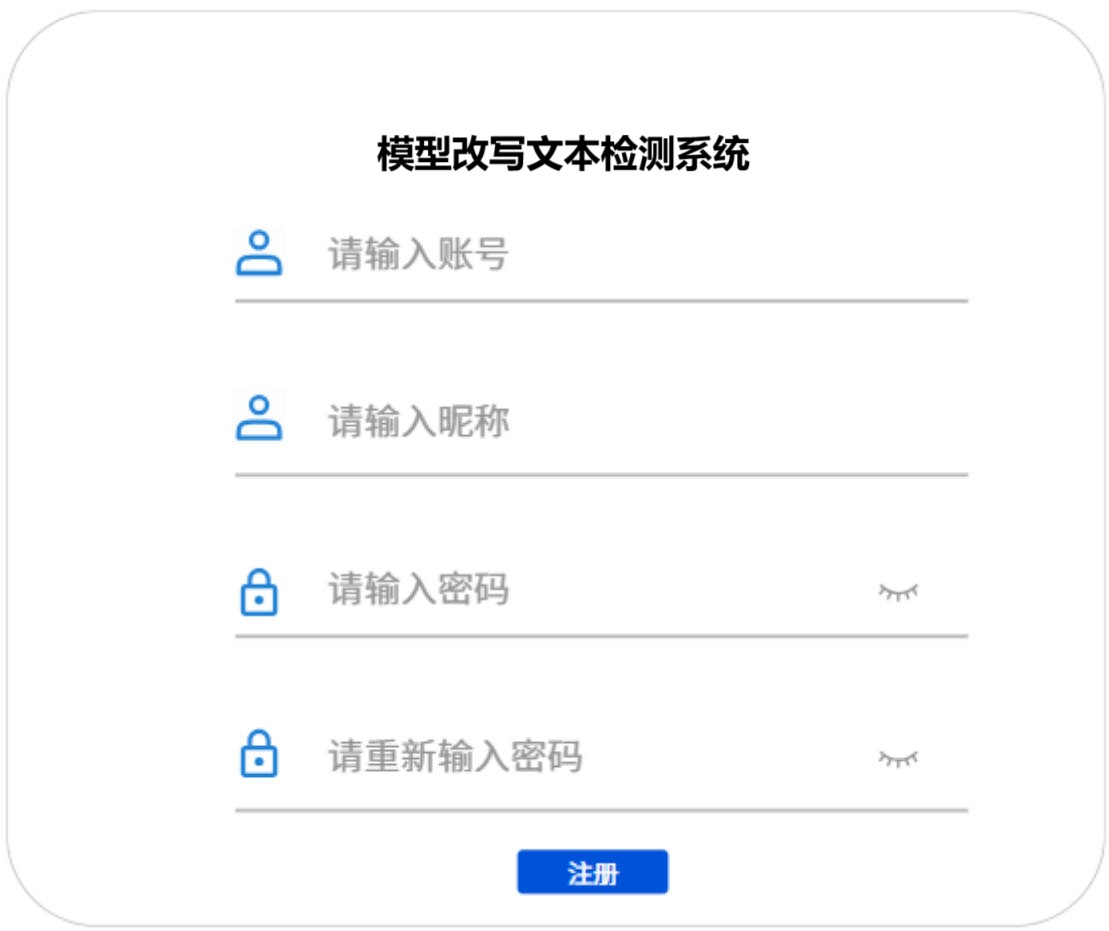
\includegraphics[width=0.45\textwidth]{figures/sys-register.jpg}
    }
    \caption{模型改写文本检测系统用户注册与登录}
    \label{fig:sys-login-register}
\end{figure*}

\subsection{文本改写功能}

用户成功登录系统后,可以进行文本改写操作,具体界面如图 \ref{fig:sys-polish} 所示。在此过程中,用户需输入待改写的文本,系统将利用相应的模型进行处理,并返回改写后的结果。用户可以查看并下载生成的文本。此外,系统允许用户选择不同的改写模型,以便进行针对性的文本处理。用户也可以对改写后的文本进行进一步编辑和修改,以满足个人需求。

\begin{figure*}[htb]
    \centering
    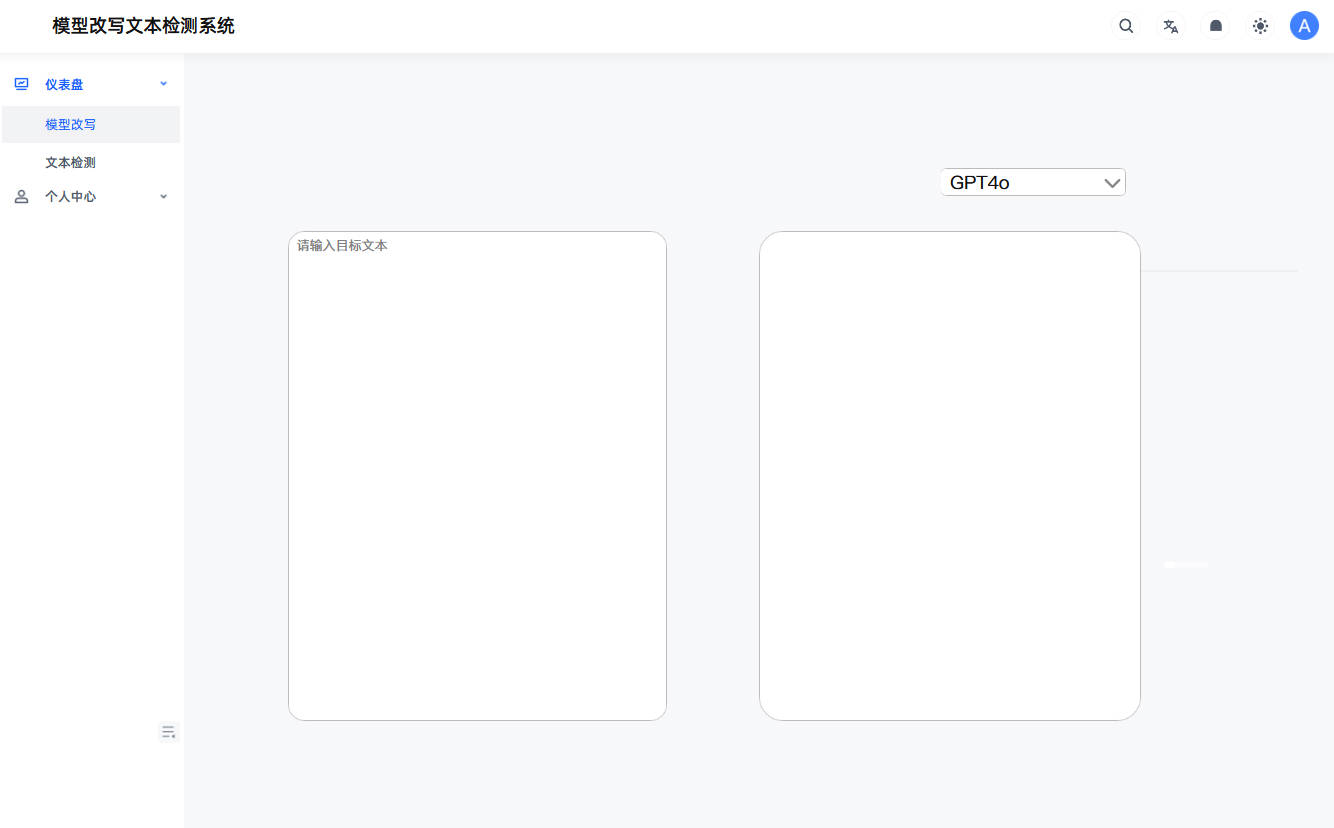
\includegraphics[width=\textwidth]{figures/sys-polish.jpg}
    \caption{模型改写文本检测系统——文本改写功能}
    \label{fig:sys-polish}
\end{figure*}

\subsection{模型改写文本检测功能}

在用户成功登录后,系统提供了模型改写文本检测的功能,具体界面如图 \ref{fig:sys-detect} 所示。用户可以输入待检测的文本,系统将运用相应的模型进行分析,并返回检测结果,检测后结果如图 \ref{fig:sys-detect2} 所示。用户有权查看并下载这些检测结果。此外,系统允许用户在后台选择不同的检测模型,以便为文本检测提供更为精确的处理,系统将依据用户的选择执行相应的操作。

\begin{figure*}[htb]
    \centering
    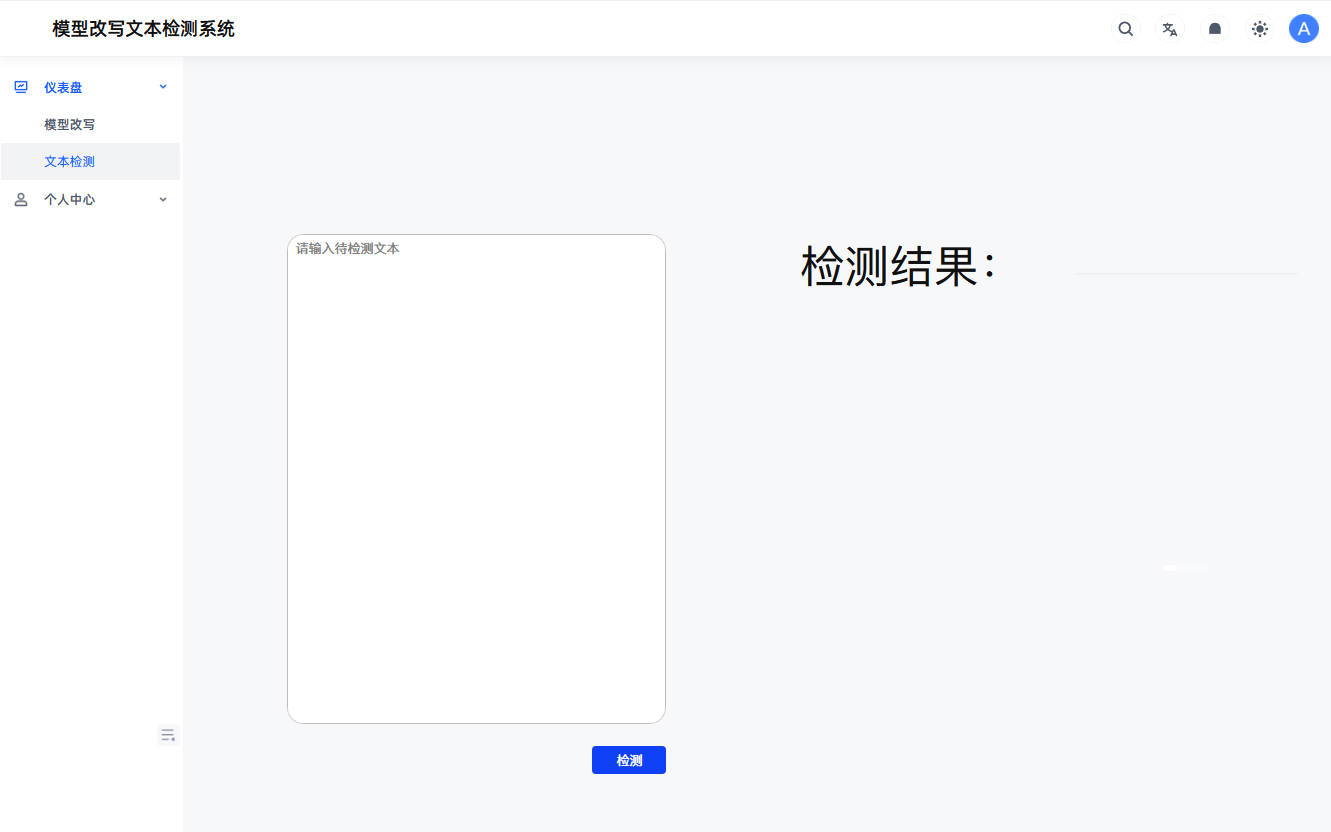
\includegraphics[width=\textwidth]{figures/sys-detect.jpg}
    \caption{模型改写文本检测系统——模型改写文本检测功能——检测前}
    \label{fig:sys-detect}
\end{figure*}

\begin{figure*}[htb]
    \centering
    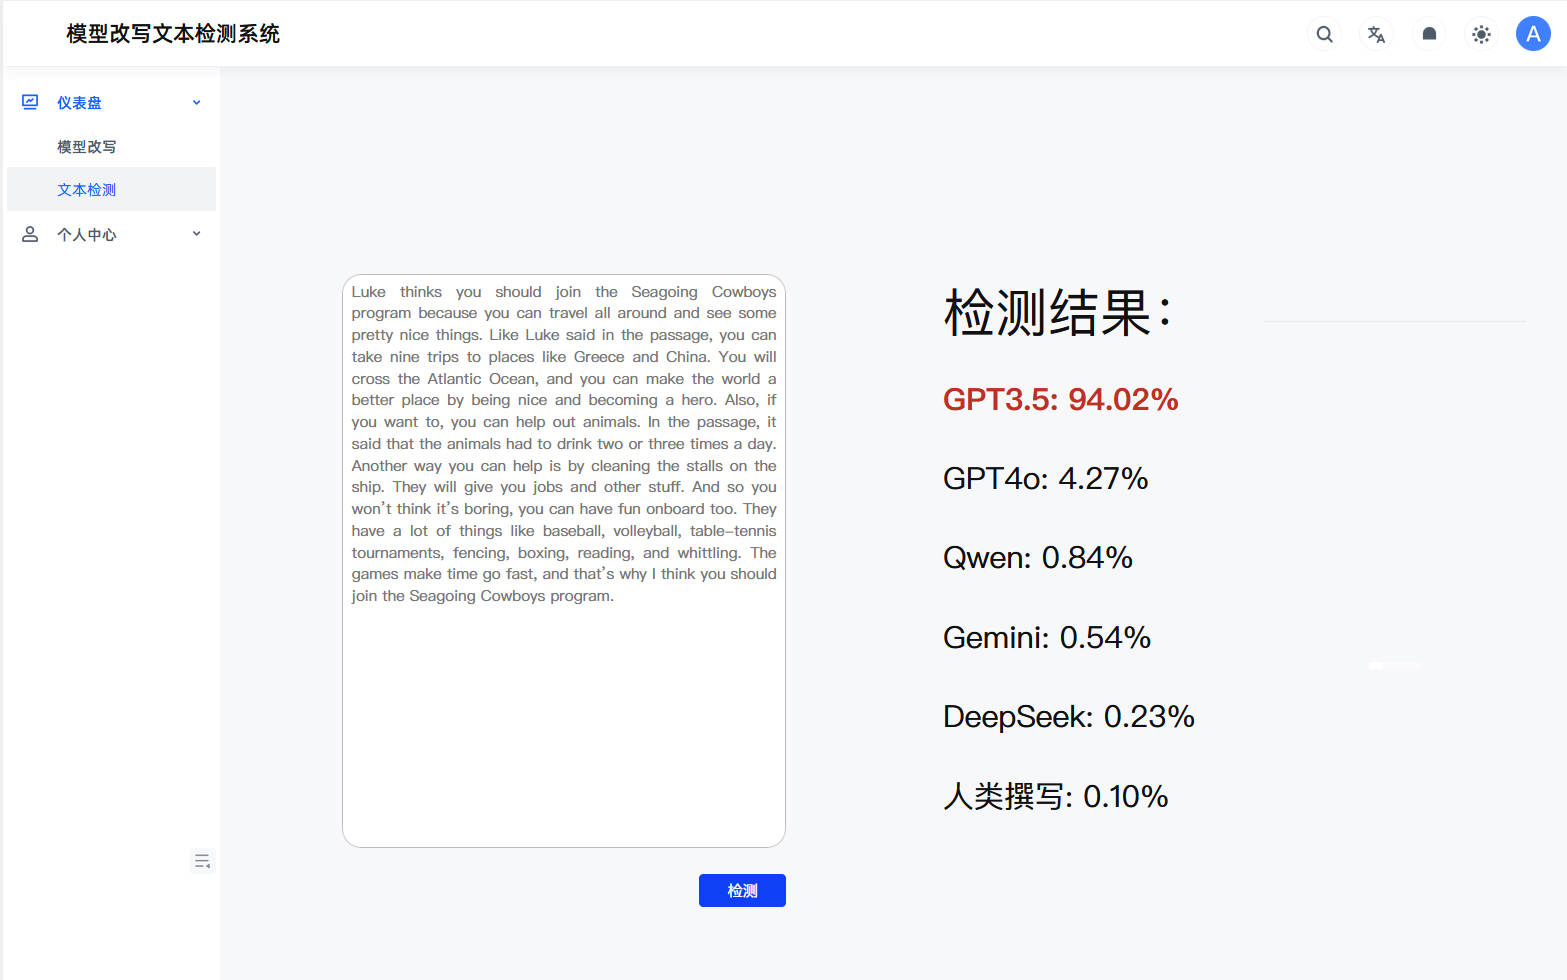
\includegraphics[width=\textwidth]{figures/sys-detect2.jpg}
    \caption{模型改写文本检测系统——模型改写文本检测功能——检测后}
    \label{fig:sys-detect2}
\end{figure*}

\section{本章小结}
\label{sec:sys-conclusion}

本章主要介绍了模型改写文本检测系统的设计与实现,包括需求分析、系统架构设计、模块和接口设计以及数据库设计。通过对系统的功能进行详细分析,明确了系统的业务需求和功能需求,为后续的系统实现提供了基础。系统采用前后端分离的架构设计,提高了系统的灵活性和可扩展性。通过模块和接口设计,明确了系统各个模块之间的关系和数据传输方式。数据库设计则为系统的数据存储提供了支持。最后,通过用户注册与登录、文本改写功能、模型改写文本检测功能等展示了系统的实际应用效果。

本章为模型改写文本检测系统的设计与实现奠定了基础,为后续的系统测试和优化提供了依据。通过对系统的设计与实现,可以看出模型改写文本检测系统在实际应用中的可行性和有效性,为后续的研究和应用提供了参考。

\backmatter

% 结论
%%
% The BIThesis Template for Graduate Thesis
%
% Copyright 2020-2023 Yang Yating, BITNP
%
% This work may be distributed and/or modified under the
% conditions of the LaTeX Project Public License, either version 1.3
% of this license or (at your option) any later version.
% The latest version of this license is in
%   https://www.latex-project.org/lppl.txt
% and version 1.3 or later is part of all distributions of LaTeX
% version 2005/12/01 or later.
%
% This work has the LPPL maintenance status `maintained'.
%
% The Current Maintainer of this work is Feng Kaiyu.

\begin{conclusion}

一、本文工作

本文针对教育领域的人工智能文本滥用、目前模型改写文本检测数据集细粒度数
据不足等问题,提出了新的研究框架并构建了模型改写文本检测数据集,提出了一种文档级文本检测方法,并构建了模型改写文本检测系统,实现显示了方法在文档级任务上的表现,显示出其在处理复杂文本结构方面的能力。本文主要贡献如下:

(1)提出了一个新的模型改写文本检测数据集,包含了多种大语言模型生成的文本样本,以句子的细粒度涵盖了多种模型改写文本。该数据集为研究人员提供了一个有价值的资源,以评估和比较不同的文本检测方法。

(2)提出了一种基于句子级文本检测技术的文档级文本检测方法。该方法通过
分层处理解决长文本建模难题,引入注意力机制保留上下文语义,并建立了端到端的可微分计算流程,从而基于句子级文本检测完成文档级文本检测,实验证验了该方法能有效地识别大语言模型生成的文本。

(3)搭建了一个模型改写文本检测系统,提供了用户友好的界面和高效的文本检测功能。该系统可以帮助教育工作者和研究人员快速识别和分析学生的写作风格和文本来源,为教育领域的文本检测提供了实用的解决方案。

二、未来工作与展望

本文针对目前的大语言模型生成文本检测数据集的细粒度数据不足、无法检测出一段文本具体由哪种大语言模型生成的问题,提出了模型生成文本检测数据集,但仍存在进一步探索空间,未来工作可以从以下方面进行改进:

(1)未来研究可重点优化句子级文本检测,并构建更丰富的数据集来提升模型性能。具体可从两方面着手:一是深入分析生成文本的词汇、句法和语义特征以提高检测精度;二是建立覆盖多领域、多语言的数据集来增强泛化能力。同时,随着生成模型的快速进化,检测方法需持续创新,可引入在线学习或元学习策略来动态适应新型文本。此外,还需优化模型计算效率,平衡实时场景下的检测速度与准确性。这些改进将推动文本检测技术的实际应用。

(2)此外,结合其他技术(如图神经网络或迁移学习)可能为这一领域带来新的突破。图神经网络能够有效捕捉文本中复杂的语义关系网络,有助于识别生成文本中隐藏的模式特征;而迁移学习则可以利用预训练语言模型的知识,快速适应不同领域的文本检测任务。通过融合这些先进技术,不仅可以提升模型对生成文本的判别能力,还能增强其在跨领域、跨语言场景下的适应性和鲁棒性。这种多技术融合的研究思路,将为生成文本检测开辟更广阔的发展空间。

(3)本文搭建的系统目前仍存在一些不足之处,如功能过少、管理员仍需要从命令行操作用户等。未来的开发可以集中在改进系统的用户体验和功能扩展上,以满足更广泛的需求。首先,可以开发更直观的图形化管理界面,让管理员能够通过可视化操作完成用户管理、权限设置等日常工作,减少对命令行操作的依赖。其次,系统功能模块需要进一步丰富,比如增加数据分析、自动化报告生成等实用功能,提升系统的整体价值。此外,响应速度和操作流畅度也有待优化,通过改进前后端交互机制和缓存策略,可以显著提升用户的使用体验。这些改进方向将帮助系统更好地服务于目标用户群体。

\end{conclusion}

% 参考文献
%%
% The BIThesis Template for Graduate Thesis
%
% Copyright 2020-2023 Yang Yating, BITNP
%
% This work may be distributed and/or modified under the
% conditions of the LaTeX Project Public License, either version 1.3
% of this license or (at your option) any later version.
% The latest version of this license is in
%   https://www.latex-project.org/lppl.txt
% and version 1.3 or later is part of all distributions of LaTeX
% version 2005/12/01 or later.
%
% This work has the LPPL maintenance status `maintained'.
%
% The Current Maintainer of this work is Feng Kaiyu.

%
% 如无特殊需要,本页面无需更改。
%
% **注意:如果发现渲染出来的文献编号不正确,请同时使用以下两个方式解决:**
% 1. 清除缓存后重新编译(比如使用 `latexmk -c`)。
% 2. 请确保无编译错误。


\begin{bibprint}
  \printbibliography[heading=none,notcategory=mypub,resetnumbers=true]
\end{bibprint}


% 附录
% %%
% The BIThesis Template for Graduate Thesis
%
% Copyright 2020-2023 Yang Yating, BITNP
%
% This work may be distributed and/or modified under the
% conditions of the LaTeX Project Public License, either version 1.3
% of this license or (at your option) any later version.
% The latest version of this license is in
%   https://www.latex-project.org/lppl.txt
% and version 1.3 or later is part of all distributions of LaTeX
% version 2005/12/01 or later.
%
% This work has the LPPL maintenance status `maintained'.
%
% The Current Maintainer of this work is Feng Kaiyu.

\begin{appendices}
  \chapter{费马大定理的证明}
  关于此,我确信已发现了一种美妙的证法,可惜这里空白的地方太小,写不下。

  \chapter{Maxwell Equations}
  因为在柱坐标系下,$\overline{\overline\mu}$是对角的,所以Maxwell方程组中电场$\bf
  E$的旋度

  所以$\bf H$的各个分量可以写为:
  \begin{subequations}
    \begin{eqnarray}
      H_r=\frac{1}{\mathbf{i}\omega\mu_r}\frac{1}{r}\frac{\partial
        E_z}{\partial\theta } \\
      H_\theta=-\frac{1}{\mathbf{i}\omega\mu_\theta}\frac{\partial E_z}{\partial r}
    \end{eqnarray}
  \end{subequations}

  同样地,在柱坐标系下,$\overline{\overline\epsilon}$是对角的,所以Maxwell方程组中磁场$\bf
  H$的旋度
  \begin{subequations}
    \begin{eqnarray}
      &&\nabla\times{\bf H}=-\mathbf{i}\omega{\bf D}\\
      &&\left[\frac{1}{r}\frac{\partial}{\partial
          r}(rH_\theta)-\frac{1}{r}\frac{\partial
          H_r}{\partial\theta}\right]{\hat{\bf
          z}}=-\mathbf{i}\omega{\overline{\overline\epsilon}}{\bf
        E}=-\mathbf{i}\omega\epsilon_zE_z{\hat{\bf z}} \\
      &&\frac{1}{r}\frac{\partial}{\partial
        r}(rH_\theta)-\frac{1}{r}\frac{\partial
        H_r}{\partial\theta}=-\mathbf{i}\omega\epsilon_zE_z
    \end{eqnarray}
  \end{subequations}

  由此我们可以得到关于$E_z$的波函数方程:
  \begin{eqnarray}
    \frac{1}{\mu_\theta\epsilon_z}\frac{1}{r}\frac{\partial}{\partial r}
    \left(r\frac{\partial E_z}{\partial r}\right)+
    \frac{1}{\mu_r\epsilon_z}\frac{1}{r^2}\frac{\partial^2E_z}{\partial\theta^2}
    +\omega^2 E_z=0
  \end{eqnarray}

  \chapter{要求}

  \textcolor{blue}{
  有些材料编入文章主体会有损于编排的条理性和逻辑性,或有碍于文章结构的紧凑和突出主题思想等,这些材料可作为附录另页排在参考文献之后,也可以单编成册。下列内容可作为附录:
  }
  \begin{enumerate}
    \item \textcolor{blue}{为了整篇论文材料的完整,但编入正文有损于编排的条理性和逻辑性的材料,这一类材料包括比正文更为详尽的信息、研究方法和技术等更深入的叙述,以及建议可阅读的参考文献题录和对了解正文内容有用的补充信息等;}
    \item \textcolor{blue}{ 由于篇幅过大或取材的复制资料不便于编入正文的材料; }
    \item \textcolor{blue}{ 不便于编入正文的罕见珍贵资料; }
    \item \textcolor{blue}{ 一般读者无须阅读,但对本专业同行有参考价值的资料; }
    \item \textcolor{blue}{ 某些重要的原始数据、推导、计算程序、框图、结构图、注释、统计表、计算机打印输出件等; }
  \end{enumerate}

  \section{一级标题}
  \subsection{二级标题}
\end{appendices}


% 个人成果
%%
% The BIThesis Template for Graduate Thesis
%
% Copyright 2020-2023 Yang Yating, BITNP
%
% This work may be distributed and/or modified under the
% conditions of the LaTeX Project Public License, either version 1.3
% of this license or (at your option) any later version.
% The latest version of this license is in
%   https://www.latex-project.org/lppl.txt
% and version 1.3 or later is part of all distributions of LaTeX
% version 2005/12/01 or later.
%
% This work has the LPPL maintenance status `maintained'.
%
% The Current Maintainer of this work is Feng Kaiyu.

% 1. 在 `./reference/pub.bib` 中添加数据。
% 2. 在下方 `\addpubs` 添加该文献(参考下方示例)。

% **注意:如果发现渲染出来的文献编号不正确,请同时使用以下两个方式解决:**
% 1. 请清除缓存后重新编译(比如使用 `latexmk -c`)。
% 2. 请确保无编译错误。

\begin{publications}

  % **默认情况下,这里的内容将按照学校要求,以发表时间排序。**
  % - 如果想要按照引用顺序排序,可以开启 `publications/sorting` 选项。
  % - 如果想要微调,详见 https://bithesis.bitnp.net/faq/bib-sort.html#sortkey 。
  % 更多信息请参考「bithesis.pdf」手册。
  \addpubs{DBLP:journals/apin/YinLLSL24}
  \addpubs{TOSWT}

  % 主要针对硕士生
  \printbibliography[heading=none,category=mypub,resetnumbers=true]

  % 如果想要分为多个列表,可以使用以下的命令。
  % 主要针对博士生。
  % \pubsection{文章}
  % \printbibliography[heading=none,type=article,category=mypub,resetnumbers=true]{}
  %
  % \pubsection{一些书}
  % \printbibliography[heading=none,type=book,category=mypub,resetnumbers=true,notkeyword=dummy]{}
  %
  % \pubsection{另一些书}
  % \printbibliography[heading=none,type=book,category=mypub,keyword=dummy,resetnumbers=true]{}
  %
  % 关于 \printbibliography 的筛选参数:
  % 0. 请保留“category=mypub”。(这样只列出成果,不列出正文参考文献。)
  % 1. 设置“type=…”,每次只输出某一类型。
  % 2. 若需继续细分,请在 pub.bib 的条目里记录“keywords = {…, …}”,然后在此用“keyword=…”筛选。
  % 3. 如果还有要求,可用notkeyword、subtype等筛选方法,请参考 biblatex 手册。

  % 如果想绕过 pub.bib 直接记录项目(例如获奖),请参考以下内容,
  % 定义一个能和 \printbibliography 共存的列表。
  % https://bithesis.bitnp.net/faq/pub-manual.html
  % \zihao{5} % 字号改为五号
  % \renewcommand{\labelenumi}{[\theenumi]} % 编号改用中括号
  
  % \begin{enumerate}[nosep, leftmargin=4ex-2pt, labelsep=1ex]
  %   \setcounter{enumi}{1} % 下一项为 5。
  %   \item ***[J]. Applied Intelligence, 2024, 54(7): 5891-5906.
  %   \item ***[C]. Proceedings of the 2025 13th International Conference on Information and Education Technology. 2025.
  % \end{enumerate}
\end{publications}


% 致谢
%%
% The BIThesis Template for Graduate Thesis
%
% Copyright 2020-2023 Yang Yating, BITNP
%
% This work may be distributed and/or modified under the
% conditions of the LaTeX Project Public License, either version 1.3
% of this license or (at your option) any later version.
% The latest version of this license is in
%   https://www.latex-project.org/lppl.txt
% and version 1.3 or later is part of all distributions of LaTeX
% version 2005/12/01 or later.
%
% This work has the LPPL maintenance status `maintained'.
%
% The Current Maintainer of this work is Feng Kaiyu.

\begin{acknowledgements}

恍恍惚惚,硕士研究生三年时光飞逝,我要毕业迈向工作了。从刚进入北京理工大学的战战兢兢,到如今即将离校的依依不舍,心中感慨万千。感谢母校的培养,感谢老师的教导,感谢同学的陪伴,感谢朋友的支持。

在此,我要特别感谢导师李侃老师和网络信息中心的屈少杰老师,是您们悉心的指导和无私的帮助,让我在研究中不断成长。李老师的严谨治学和屈老师的热情支持让我在科研道路上走得更加坚定。

感谢我的同门师兄弟姐妹们,感谢你们在我研究生生活中给予的支持和帮助。我们一起度过了无数个难忘的时光,分享了彼此的快乐与烦恼。你们的陪伴让我在这段旅程中不再孤单。

感谢我的家人,感谢你们一直以来的支持和理解。无论我身处何地,你们始终是我最坚实的后盾。你们的爱让我在追求梦想的道路上充满力量。

\end{acknowledgements}

% 个人简介(仅博士生需要此项)
% %%
% The BIThesis Template for Graduate Thesis
%
% Copyright 2020-2023 Yang Yating, BITNP
%
% This work may be distributed and/or modified under the
% conditions of the LaTeX Project Public License, either version 1.3
% of this license or (at your option) any later version.
% The latest version of this license is in
%   https://www.latex-project.org/lppl.txt
% and version 1.3 or later is part of all distributions of LaTeX
% version 2005/12/01 or later.
%
% This work has the LPPL maintenance status `maintained'.
%
% The Current Maintainer of this work is Feng Kaiyu.

\begin{resume}

本人…。

\textcolor{blue}{
  硕士学位论文不必提供作者简介。博士学位论文应该提供作者简介,主要包括:姓名、性别、出生年月、民族、出生地;简要学历、工作经历(职务);攻读学位期间取得的其他研究成果或奖励。
}

\end{resume}


% 在全文最后,博士附《博士学位论文答辩表》前2页决议含签字的扫描版,硕士不用附。
% 建议用 Word 模板填写该表,扫描后拼接 PDF。

\end{document}
